\chapter{Sophisticated Solvers for Fast Sampling}\label{ch:solvers}


The generation process of a diffusion model, which maps noise to data samples, is mathematically equivalent to solving either an SDE or its associated ODE. This procedure is inherently slow, since it relies on numerical solvers that approximate solution trajectories with many small integration steps (see \Cref{app:de} for a brief introduction). Accelerating inference has therefore become a central research objective. Broadly, existing approaches fall into two categories:
\begin{itemize}
    \item \textbfs{Training-Free Approaches:} The focus of this chapter. These methods develop advanced numerical solvers to improve the efficiency of diffusion sampling without additional training.
    \item \textbfs{Training-Based Approaches:} Covered in \Cref{ch:distillation,ch:fast-scratch}. These techniques either distill a pre-trained diffusion model into a fast generator, or directly learn the ODE flow map (solution) so that only a few sampling steps are required.
\end{itemize}
SDE-based samplers (e.g., Euler--Maruyama) may yield more diverse samples due to stochasticity but typically require more steps~\citep{xu2023restart}. Here we focus on ODE-based generation, whose principles extend naturally to the SDE setting.




\clearpage




\section{Prologue}
\subsection{Advanced Solvers for Diffusion Models}

The Score SDE framework~\citep{song2020score} established a key foundation by rigorously linking the discrete-time diffusion and ELBO formulations~\citep{sohl2015deep,ho2020denoising} with the continuous-time SDE/ODE perspective of generative modeling. This unification not only provides theoretical clarity but also enables principled development of efficient sampling algorithms based on numerical integration.

Concretely, suppose we have a pre-trained diffusion model $\rvs_{\bm{\phi}^\times}(\rvx, t) \approx \nabla_{\rvx}\log p_t(\rvx)$ (which admits the other three equivalent expressions as in \Cref{sec:equivalent-parametrizations}). 
In this case, the sampling procedure can be viewed as solving the PF-ODE with initial condition $\rvx(T) \sim p_{\text{prior}}$, integrated backward in time from $t = T$ down to $t = 0$:
\begin{align*}
    \frac{\diff \rvx(t)}{\diff t} 
     =  \rvf(\rvx(t),t) 
    - \frac{1}{2} g^2(t) \underbrace{\nabla_{\rvx}\log p_t(\rvx(t))}_{\approx\,  \rvs_{\bm{\phi}^\times}(\rvx(t), t)}.
\end{align*}
This ODE is directly associated with the forward stochastic process
\[
\diff\rvx(t) = \rvf(\rvx(t),t)\diff t + g(t)\diff\rvw(t),
\]
showing the continuous-time connection between the generative (reverse-time) and noising (forward-time) dynamics.

The exact solution of the PF-ODE can be written equivalently in integral form:
\begin{align}\label{eq:solution-int-score}
\begin{aligned}
    \bPsi_{T\to 0} \left(\rvx(T)\right) 
    &= \rvx(T) + \int_T^0  \Big[f(\tau)\rvx(\tau) - \frac{1}{2}g^2(\tau) \nabla_{\rvx}\log p_\tau(\rvx(\tau))\Big]\diff \tau \\
    &\approx \rvx(T) + \int_T^0  \Big[f(\tau)\rvx(\tau) - \frac{1}{2}g^2(\tau) \rvs_{\bm{\phi}^\times} \big(\rvx(\tau), \tau\big)\Big]\diff \tau \\
    &=:\widetilde\bPsi_{T\to 0} \left(\rvx(T)\right).
\end{aligned}
\end{align}
Here, $\bPsi_{s\to t}(\rvx)$ denotes the flow map of the \emph{oracle} PF-ODE, mapping a state $\rvx$ at time $s$ to its evolved state at time $t$ (see \Cref{eq:flow-map-def}). In contrast, $\widetilde\bPsi_{s\to t}(\rvx)$ denotes the flow map of the \emph{empirical} PF-ODE, obtained by replacing the true diffusion model $\nabla_{\rvx}\log p_t(\rvx)$ with its learned approximation $\rvs_{\bm{\phi}^\times}(\rvx,t)$. Thus, $\widetilde\bPsi_{s\to t}  \approx  \bPsi_{s\to t}$.

Since the integral form of $\widetilde\bPsi_{s\to t}$ cannot be evaluated in
closed form, sampling must rely on \emph{numerical solvers}. These methods
approximate the solution by discretizing time and replacing the continuous
integral with a finite sum of local drift  evaluations, thereby tracing an
approximate trajectory. Such solver-based integral approximations are referred
to as \emph{training-free} algorithms for fast diffusion sampling, since they aim
to approximate the PF-ODE solution directly from the frozen pre-trained score
model $\rvs_{\bm{\phi}^\times}$ without requiring any additional learning.

Below we first detail the common concept of numerical solvers and introduce the notations used later.  

\paragraph{Discretized Approximation of Continuous Trajectories.}  
Let $\rvx_T$ denote the initial state at time $T$, and consider a decreasing partition
\begin{align}\label{eq:time-step-def}
    T = t_0 > t_1 > \cdots > t_M = 0.
\end{align}
Starting from $\tilde{\rvx}_{t_0} = \rvx_T \sim p_{\mathrm{prior}}$, the solver produces a sequence $\{\tilde{\rvx}_{t_i}\}_{i=0}^M$ that ideally approximates the empirical PF-ODE flow $\widetilde\bPsi_{T\to t_i}(\rvx_T)$, itself a proxy for the oracle map $\bPsi_{T\to t_i}(\rvx_T)$. Each numerical step advances the state via this empirical velocity field, and the final iterate $\tilde{\rvx}_{t_M}$ serves as an estimate of the clean sample $\rvx_0$ at $t=0$.




% \paragraph{Discretized Approximation of the Continuous Trajectory.}  
% Formally, let $\rvx_T$ denote the initial state at time $T$, and consider a decreasing partition
% \begin{align}\label{eq:time-step-def}
%     t_0 = T > t_1 > \cdots > t_M = 0.
% \end{align}
% Starting from $\tilde{\rvx}_{t_0} = \rvx_T \sim p_{\mathrm{prior}}$, the solver generates a sequence $\{\tilde{\rvx}_{t_i}\}_{i=0}^M$, where, ideally, each iterate $\tilde{\rvx}_{t_i}$ would approximate the oracle PF-ODE flow $\bPsi_{T\to t_i}(\rvx_T)$. In practice, the model only has access to an empirical velocity field (via the learned diffusion model’s score), so the solver instead tracks the empirical PF-ODE solution $\widetilde\bPsi_{T\to t_i}(\rvx_T)$. Each numerical step advances the state using this empirical velocity field, and the final iterate $\tilde{\rvx}_{t_M}$ serves as an estimate of the desired clean sample $\rvx_0$ at $t=0$.


\subsection{A Common Framework for Designing Solvers in Literature}\label{subsec:common_design_solvers}

\citet{zhang2022fast,zhang2023gddim} highlighted three practical principles for designing numerical solvers for the PF-ODE associated with diffusion models.

\paragraph{I. Semilinear Structure.}
Although \citet{song2020score} establish the foundation for a general drift $\rvf(\rvx(t),t)$,  
in most scheduler formulations the drift is instantiated in a linear form
\[
\rvf(\rvx, t) := f(t)\,\rvx, \quad f:\mathbb{R}\to\mathbb{R},
\]
which induces the PF-ODE in a \emph{semilinear} structure:
\begin{equation}\label{eq:score_pf-ode}
    \frac{\diff\rvx(t)}{\diff t}
     = 
    \underbrace{f(t) \rvx(t)}_{\text{linear part}}
     - 
    \underbrace{\tfrac{1}{2} g^2(t) \rvs_{\bm{\phi}^\times}(\rvx(t), t)}_{\text{nonlinear part}}.
\end{equation}
This linear–nonlinear split in $\rvx$ is advantageous for accuracy and stability and motivates specialized integrators (see discussion near \Cref{eq:variation_of_constants} below)~\citep{hochbruck2005explicit,hochbruck2010exponential}.



\paragraph{II. Parameterizations beyond the Score.}
As $t \to 0$, the true score $\nabla_{\rvx}\log p_t(\cdot)$ can change very
rapidly (for example, when $p_{\text{data}}$ is concentrated near a
low-dimensional manifold)~\citep{kim2022soft}. This makes it difficult for a neural network
$\rvs_{\bphi^\times}$, which is trained to approximate the score directly, to
remain accurate. 

To see why, recall the oracle relation (see \Cref{eq:predictions-equivalence})
\[
\beps^*(\rvx_t,t) = -\sigma_t \nabla_{\rvx}\log p_t(\rvx_t),
\]
where $\beps^*(\rvx_t,t)=\mathbb{E}[\beps |\rvx_t]$ is the oracle noise, and $(\alpha_t,\sigma_t)$ are the mean and standard deviation of the
perturbation kernel 
$\rvx_t |\rvx_0 \sim \mathcal{N}(\alpha_t \rvx_0, \sigma_t^2 I)$,
connected to $f(t),g(t)$ via \Cref{eq:kernel-sde-equiv}. From the orthogonality property in $L^2$,
\[
\mathbb{E}\,\|\beps\|_2^2
=\mathbb{E}\,\|\beps^*\|_2^2+\mathbb{E}\,\|\beps-\beps^*\|_2^2
\;\;\Rightarrow\;\;
\mathbb{E}\,\|\beps^*\|_2^2 \leq \mathbb{E}\,\|\beps\|_2^2 = D.
\]
Hence the oracle noise predictor is always bounded, but the score grows like
\[
\mathbb{E}\,\|\rvs^*(\rvx_t,t)\|_2^2
= \sigma_t^{-2}\,\mathbb{E}\,\|\beps^*(\rvx_t,t)\|_2^2
 \leq  \frac{D}{\sigma_t^2}.
\]
Thus, as $t\to 0$, the score can blow up at the rate $1/\sigma_t^2$, while the
noise predictor stays bounded. Because neural networks can only approximate
smoothly growing functions, score prediction tends to be numerically unstable
and less accurate, which in turn can harm numerical PF-ODE solvers when relying
on a pre-trained model as a drift.

For this reason, a widely used alternative is to predict the noise
$\beps_{\bm{\phi}^\times}$ (or its variants such as $\rvx$- or $\rvv$-prediction),
which is stably bounded and admits a simple closed-form relation to the score:
\[
\rvs_{\bm{\phi}^\times}(\rvx,t) = -\frac{1}{\sigma_t}\,\beps_{\bm{\phi}^\times}(\rvx,t).
\]



Substituting this relation into the PF-ODE (cf.\ \Cref{eq:clean_pf_ode}) gives
\begin{equation}\label{eq:noise_pf_ode}
\frac{\diff\rvx(t)}{\diff t}
 = 
\underbrace{f(t) \rvx(t)}_{\text{linear part}}
 + 
\underbrace{\tfrac{1}{2} \tfrac{g^2(t)}{\sigma_t} \beps_{\bm{\phi}^\times}(\rvx(t), t)}_{\text{nonlinear part}}.
\end{equation}
This parameterization is commonly adopted by modern PF-ODE solvers.

\paragraph{III. Exponential Integrators for semilinear PF-ODEs.} 
For the semilinear structure in \Cref{eq:noise_pf_ode}, the \emph{exponential integrator formula} in \Cref{eq:variation_of_constants} provides an exact alternative representation of the solution.
 To see this, let $\rvx_s$ denote the state at start time $s$, and let $t\in[0,s]$ be the terminal time\footnote{Here, $s$ is the start time and $t$ the terminal time, so sampling integrates backward with $s>t$.}. 
 
 For clarity, write the nonlinear part of \Cref{eq:noise_pf_ode} as
\[
\rmN(\rvx(t), t) := \frac{1}{2}\frac{g^2(t)}{\sigma_t}\,\beps_{\bm{\phi}^\times}(\rvx(t), t).
\]
The ODE can then be written as
\begin{align}\label{eq:general-semilinear-pfode}
    \frac{\diff \rvx(t)}{\diff t} - \underbrace{f(t)\rvx(t)}_{\text{linear part}} = \underbrace{\rmN(\rvx(t), t)}_{\text{nonlinear part}}.
\end{align}
To isolate the linear term, we introduce the \emph{exponential integrator}
\[
\mathcal{E}(s \shortrightarrow t) \coloneqq \exp \Bigl(\int_s^t f(u) \diff u\Bigr),
\]
and multiply both sides of the ODE by its inverse $\mathcal{E}(t \shortrightarrow s)$.
By the product rule,
\[
\mathcal{E}^{-1}(s \shortrightarrow t) \left(\frac{\diff \rvx(t)}{\diff t} - f(t)\rvx(t)\right)
= \frac{\diff}{\diff t}\Big[\,\mathcal{E}^{-1}(s \shortrightarrow t)\rvx(t)\,\Big].
\]
Hence the equation becomes
\[
\frac{\diff}{\diff t}\Big[\,\mathcal{E}^{-1}(s \shortrightarrow t)\rvx(t)\,\Big]
= \mathcal{E}^{-1}(s \shortrightarrow t)\,\rmN(\rvx(t), t).
\]
Integrating from $s$ to $t$ and then multiplying back by $\mathcal{E}(s \shortrightarrow t)$ gives the solution:
\begin{mdframed}
    \begin{equation}\label{eq:variation_of_constants}
\widetilde\bPsi_{s\to t}(\rvx_s)
= \underbrace{\mathcal{E}(s \shortrightarrow t)\rvx_s}_{\text{linear part}}
+ \frac{1}{2}\int_s^t \frac{g^2(\tau)}{\sigma_\tau} 
\mathcal{E}(\tau \shortrightarrow t) 
\beps_{\bm{\phi}^\times}(\rvx_\tau,\tau) \diff\tau.
\end{equation}
\end{mdframed}
We refer the reader to \Cref{app:exp-int-factor} for the full details of the derivation.

To explain why the exponential–integration form in \Cref{eq:variation_of_constants} is preferable to \Cref{eq:noise_pf_ode} for few-step sampling (large $\Delta s$), we compare their one–step updates. Using variation of constants, $\mathcal{E}(s\shortrightarrow s-\Delta s)=e^{-f(s)\Delta s}$ and freezing $\rmN(\rvx(\tau),\tau)\approx \rmN(\rvx_s,s)$ for $\tau\in[s-\Delta s,s]$, the exponential–Euler update of \Cref{eq:variation_of_constants} is
\begin{align}\label{eq:exp-euler-step}
&\rvx^{\mathrm{Exp}\text{-}\mathrm{Euler}}_{s-\Delta s}
= \underbrace{e^{-f(s)\Delta s}\rvx_s}_{\text{linear part}}
+\underbrace{\frac{e^{-f(s)\Delta s}-1}{f(s)}\,\rmN(\rvx_s,s)}_{\text{nonlinear part}},
\end{align}
with the natural limit $\bigl(e^{-f\Delta s}-1\bigr)/f\to -\Delta s$ as $f\to 0$. Here the linear factor $e^{-f(s)\Delta s}$ is exactly computed (no approximation).

In contrast, approximating $f(\tau)\rvx_\tau - \rmN(\rvx_\tau,\tau)\approx f(s)\rvx_s - \rmN(\rvx_s,s)$ for $\tau\in[s-\Delta s,s]$ yields the plain–Euler step for \Cref{eq:noise_pf_ode}:
\begin{align}\label{eq:euler-step}
  \rvx^{\mathrm{Euler}}_{\,s-\Delta s}
=\rvx_s-\Delta s\,[\,f(s)\,\rvx_s+\rmN(\rvx_s,s)\,]
=\underbrace{(1-f(s)\Delta s)\,\rvx_s}_{\text{linear part}}
-\underbrace{\Delta s\,\rmN(\rvx_s,s)}_{\text{nonlinear part}}. 
\end{align}

The linear factor in \Cref{eq:euler-step} is the first–order Taylor approximation of the exponential in \Cref{eq:exp-euler-step}:
\[
e^{a}=1+a+\tfrac{a^2}{2}+\tfrac{a^3}{6}+\cdots,\quad a:=-f(s)\Delta s,
\]
so the gap is $e^{a}-(1+a)=\tfrac{a^2}{2}+\mathcal O(a^3)$. As soon as $|f(s)|\Delta s$ is not tiny (i.e., the step size $\Delta s$ is not sufficiently small), Euler’s linear update $(1+a)\rvx_s$ mis-scales the true factor $e^{a}\rvx_s$ by a relative error of order $a/2$. This is purely linear distortion from the discretization. The exponential–Euler step avoids it by applying the exact linear multiplier, which is especially important when taking large steps.





\subsection{Approaches of PF-ODE Numerical Solvers}
Numerical solvers for diffusion models can be broadly grouped into two categories.

\paragraph{Time Stepping Methods.}  
This class of methods discretizes the time interval $[0,T]$ and approximates the PF-ODE using various numerical integration schemes designed for efficiency. We present the most fundamental, principled, and widely adopted approaches as representative examples:

\subparagraph{Denoising Diffusion Implicit Model (DDIM).} DDIM, introduced in \Cref{sec:revisit-ddim} (with its update form already appearing in \Cref{subsec:pf-ode}), is one of the earliest fast samplers for diffusion models. Originally proposed from a variational perspective, it introduces a non-Markovian forward family whose marginals match those of the original diffusion, thereby enabling a deterministic reverse process and flexible step skipping. From the ODE viewpoint, however, DDIM can be understood more directly: it corresponds to applying a single exponential-Euler step, i.e., approximating the diffusion model term inside the integral as constant, to the exponential-integration formula \Cref{eq:variation_of_constants}, which yields the update in \Cref{eq:exp-euler-step}.

\subparagraph{Diffusion Exponential Integrator Sampler (DEIS).} 
DEIS~\citep{zhang2022fast}, introduced in \Cref{sec:exponential}, was the first to exploit the semilinear structure of the PF-ODE by applying exponential integrators. The key idea is to treat the linear part exactly via an integrating factor and approximate only the nonlinear integral term. Unlike the Euler method, which assumes a constant integrand inside the exponential integrator formula, DEIS reuses the history of previously estimated points along the trajectory. Specifically, it fits a higher-order interpolation (a \emph{Lagrange polynomial}) to the past evaluations and uses it to approximate the integral at the next step.  Geometrically, this polynomial interpolation captures the curvature of the trajectory much more accurately than a constant approximation, enabling higher-order accuracy and improved stability for large step sizes.

This reuse of past evaluations to anchor the next update (so that each
step requires only one new model call) is referred to as a
\emph{multistep method}. In contrast, a \emph{single–step method}
(e.g., DDIM) relies only on the most recent state for the next update.
Such methods are simpler but typically more costly to achieve high
accuracy, since they require more function evaluations (or more steps)
overall.

\subparagraph{The Diffusion Probabilistic Model (DPM)-Solver Family.} 
The DPM-Solver family, including DPM-Solver~\citep{lu2022dpm} (\Cref{sec:dpm}), and DPM-Solver\texttt{++}~\citep{lu2022dpm2} (\Cref{sec:dpm++}), builds on the semilinear structure of the PF-ODE with a crucial time reparameterization, the \emph{half-log signal-to-noise ratio (SNR)}:
\begin{align*}
    \lambda_t \coloneqq \frac{1}{2}\log \frac{\alpha_t^2}{\sigma_t^2} = \log \frac{\alpha_t}{\sigma_t}.
\end{align*}
This change of variables transforms the nonlinear term into an exponentially weighted integral
\[
\int_{\lambda_s}^{\lambda_t} e^{-\lambda}\,\hat{\bm{\epsilon}}_{\bm{\phi}^\times}(\hat\rvx_\lambda,\lambda) \diff \lambda,
\]
where $\hat{\bm{\epsilon}}_{\bm{\phi}^\times}$ denotes the model expressed in the reparameterized time $\lambda$ (details in \Cref{eq:analytic_solution}).  
This representation makes higher-order approximations of the  integral both more accurate.  

DPM-Solver introduced higher-order solvers by using Taylor expansions in $\lambda$, tailored to the half-log SNR reparameterization, showing that few NFEs suffice for high-quality samples. DPM-Solver\texttt{++} adapted the method to classifier-free guidance with $\rvx$-prediction for greater stability. 








\paragraph{(Optional) Time Parallel Methods.}  
A complementary strategy accelerates sampling by parallelizing computations across different time intervals, rather than processing them strictly in sequence.  

\subparagraph{ParaDiGMs.}  
Introduced in \Cref{sec:picard}, this method~\citep{shih2023parallel} reformulates the ODE solution as a fixed-point problem. This perspective allows integral terms to be evaluated in parallel, alleviating the sequential bottleneck of standard time-stepping solvers. Importantly, this approach is not limited to the exponential-integrator form; it applies equally to general PF-ODEs with nonlinear drift $\rvf(\rvx,t)$. Moreover, it is solver-agnostic: the fixed-point formulation wraps any time-stepping rule by replacing the integral with a weighted sum of model evaluations at selected times, so Euler-, DEIS-, or DPM-Solver–style updates can be used while their evaluations are performed in parallel.





\paragraph{True Computational Cost (NFEs).}
In practice, the wall–clock cost is dominated not by the number of discretization steps, but by how many
times we must call the model network. We refer to this count as the \emph{number of function evaluations
(NFE)}. If a sampler performs $m$ evaluations per step over $N$ steps, the cost scales as
\[
\mathrm{NFE} = m\,N.
\]
For example, first–order Euler or exponential–Euler schemes have $m=1$, while single–step
$k$th–order methods typically require $m\geq k$ (e.g., $k$th order of DPM-Solver). Multistep methods (e.g., DEIS, multistep version of DPM-Solver\texttt{++})
reuse past evaluations so that after a short warm-up phase the average $m$ is close to $1$.
Classifier-free guidance effectively doubles the number of calls at each step. 
Thus, in practice, ``faster'' sampling means achieving a lower NFE, not simply taking fewer steps.



\paragraph{A Remark on Using the Equivalent Form of the PF-ODE.} 
In the discussion below, we will use the results in \Cref{sec:equivalent-parametrizations}, which support the interchangeable use of the equivalent parameterizations $(f(t), g(t))$ and $(\alpha_t,\sigma_t)$ of the perturbation kernel with 
$\rvx_t | \rvx_0 \sim \mathcal{N}(\cdot;\alpha_t \rvx_0,\sigma_t^2\rmI)$, related via
\[
f(t) = \frac{\alpha_t'}{\alpha_t}, 
\quad
g^2(t) = \frac{\diff}{\diff t} \big(\sigma_t^2\big) 
         - 2 \frac{\alpha_t'}{\alpha_t} \sigma_t^2
       = 2\sigma_t\sigma_t' - 2 \frac{\alpha_t'}{\alpha_t} \sigma_t^2.
\]
Under these relations, the PF-ODE can be written in several equivalent forms (cf.\ \Cref{eq:clean_pf_ode}).


\clearpage
\newpage

\section{\texorpdfstring{DDIM}{DDIM}}\label{sec:revisit-ddim}
In this section, we introduce one of the pioneering approaches for accelerating sampling in diffusion models: \emph{Denoising Diffusion Implicit Models} (DDIM), which is also among the most widely used ODE-based solvers. Although its name suggests a variational origin, as demonstrated in \Cref{subsec:pf-ode-different-para} for $(\rvx,\beps)$-prediction, we will show that its practical update rule can also be interpreted as a straightforward application of the Euler method to approximate the integral in \Cref{eq:variation_of_constants}. This ODE perspective not only provides a principled reinterpretation of DDIM, but also lays a foundation for designing more flexible and efficient fast samplers.

The original variational derivation of DDIM will be revisited in \Cref{subsec:ddim}. In \Cref{subsec:ddim-cfm}, we establish a clear correspondence between the DDIM update rule and conditional flow matching, showing that the DDIM dynamics can be interpreted as the flow learned by CFM.






\subsection{Interpreting DDIM as an ODE Solver}
Let $s > t$ denote two discrete time steps, with $s$ being the starting time and $t$ the target time for the update. To approximate the integral in \Cref{eq:variation_of_constants}, a natural choice is to fix the integrand at  $s$ (the start of the step), assuming that
\[
\bm{\epsilon}_{\bm{\phi}^\times}(\rvx_\tau, \tau) \approx \bm{\epsilon}_{\bm{\phi}^\times}(\rvx_s, s), \quad \text{for all } \tau \in [t, s].
\]
This assumption leads to an Euler update approximation (see also \Cref{eq:exp-euler-step}), which gives rise to the following update rule:
\begin{equation}\label{eq:ddim-g-sigma}
    \tilde\rvx_{t} = \mathcal{E}(s \shortrightarrow t)\tilde\rvx_{s} 
    + \left( \frac{1}{2} \int_{s}^{t} \frac{g^2(\tau)}{\sigma_\tau} \mathcal{E}(\tau \shortrightarrow t) \diff\tau \right) 
    \bm{\epsilon}_{\bm{\phi}^\times}(\tilde\rvx_{s}, s),
\end{equation}
for an initial point $\tilde\rvx_{s}$. Here, the integral becomes analytically tractable, resulting in the following practical and efficient DDIM update formula:
\proppp{DDIM = Euler Method (Exponential Euler)}{ddim-euler}{
The update rule in \Cref{eq:ddim-g-sigma}, derived by applying the Euler method to the exponential integrator form in \Cref{eq:variation_of_constants}, yields the following DDIM update:
\begin{align}\label{eq:ddim-euler}
 \tilde\rvx_{t} = \frac{\alpha_{t}}{\alpha_{s}}\tilde\rvx_{s} - \alpha_{t}\left(\frac{\sigma_{s}}{\alpha_{s}} - \frac{\sigma_{t}}{\alpha_{t}}\right)\bm{\epsilon}_{\bm{\phi}^\times}(\tilde\rvx_{s}, s).
\end{align}
}{We use \Cref{eq:kernel-sde-equiv} that
\[
f(t) = \frac{\alpha_t'}{\alpha_t}, 
\quad
g^2(t) = \frac{\diff}{\diff t} \big(\sigma_t^2\big) 
         - 2 \frac{\alpha_t'}{\alpha_t} \sigma_t^2
       = 2\sigma_t\sigma_t' - 2 \frac{\alpha_t'}{\alpha_t} \sigma_t^2.
\]
With this, we obtain 
\[
\mathcal{E}(s \shortrightarrow t) = e^{\int_{s}^{t}f(u)\diff u} = e^{\log \alpha_u\vert_{u=s}^{u=t}} = \frac{\alpha_{t}}{\alpha_{s}}. 
\]
So
\begin{align*}
    \int_{s}^{t} \frac{g^2(\tau)}{2\sigma_\tau}  e^{\int_{\tau}^{t}f(u)\diff u}  \mathrm{d}\tau
    &= \int_{s}^{t} \frac{g^2(\tau)}{2\sigma_\tau}  \frac{\alpha_t}{\alpha_\tau}  \mathrm{d}\tau \\
    &= \alpha_t \int_{s}^{t} \frac{1}{2\sigma_\tau \alpha_\tau}
    \Big( \frac{\diff \sigma_\tau^2}{\diff \tau} - 2 \frac{\diff \log \alpha_\tau}{\diff \tau} \sigma_\tau^2 \Big) \mathrm{d}\tau \\
    &= \alpha_t \int_{s}^{t} \frac{\diff}{\diff \tau} \Big(\frac{\sigma_\tau}{\alpha_\tau}\Big)  \mathrm{d}\tau \\
    &= - \alpha_t\Big(\frac{\sigma_s}{\alpha_s} - \frac{\sigma_t}{\alpha_t}\Big).
\end{align*}
}
This correspondence reveals that DDIM can be interpreted as a first-order Euler method applied to the exponential-integrator transformed semilinear PF-ODE.

\subsection{Intuition Behind DDIM with Different Parameterizations}\label{subsec:ddim-different-para}

DDIM is one of the most widely used methods for accelerating diffusion sampling and usually may take in different parametrizations (see \Cref{eq:predictions-equivalence}) other than $\beps$-prediction. In this subsection, we present reformulations under different parameterizations and later provide a more intuitive interpretation of DDIM.


\paragraph{DDIM in Different Parameterizations.}
In practice, one uses a pre-trained diffusion model expressed in one of the standard parameterizations and substitutes the corresponding predictor for the oracle target in the DDIM discretization of the PF-ODE. 
For clarity, we state the oracle version below; the implementable version follows by the replacements
\[
\bm{\epsilon}_{\bm{\phi}^\times} \approx \bm{\epsilon}^*, 
\qquad 
\rvx_{\bm{\phi}^\times} \approx \rvx^*, 
\qquad 
\rvs_{\bm{\phi}^\times} \approx \rvs^*, 
\qquad   
\rvv_{\bm{\phi}^\times} \approx \rvv^*.
\]


\cornp{DDIM in Different Parametrizations}{Let $s>t$. Starting from $\tilde\rvx_s\sim p_s$ and ending at time $t$, the DDIM update in different parametrizations are as:
\begin{align}
\begin{aligned}
    \label{eq:ddim-update-all}
        \tilde\rvx_t  & = \frac{\alpha_{t}}{\alpha_s} \tilde\rvx_s + \alpha_{t}\left(\frac{\sigma_{t}}{\alpha_{t}} -\frac{\sigma_s}{\alpha_s}  \right) \bm{\epsilon}^*(\tilde\rvx_s, s)
    \\ &=\frac{\sigma_t}{\sigma_s}\tilde\rvx_s + \alpha_s \left(\frac{\alpha_t}{\alpha_s} - \frac{\sigma_t}{\sigma_s} \right) \rvx^*(\tilde\rvx_s, s) \\
    & = \frac{\alpha_{t}}{\alpha_s} \tilde\rvx_s + \sigma_s^2 \left(\frac{\alpha_{t}}{\alpha_s}- \frac{\sigma_{t}}{\sigma_s}\right) \rvs^*(\tilde\rvx_s, s)
        \\ & = \alpha_t \underset{\substack{\approx \rvx_{\bm{\phi}^\times} \\\text{estimated clean}}}{\underbrace{\rvx^*(\tilde\rvx_s, s)}}  + \sigma_t \underset{\substack{\approx \beps_{\bm{\phi}^\times} \\\text{estimated noise}}}{\underbrace{\bm{\epsilon}^*(\tilde\rvx_s, s)}}.
\end{aligned}
\end{align}
}

The last identity in \Cref{eq:ddim-update-all} gives a clear view of DDIM: 
starting from $\tilde\rvx_s\sim p_s$, the (estimated) clean part $\rvx^*(\tilde\rvx_s,s)$ and (estimated) noise part 
$\beps^*(\tilde\rvx_s,s)$ act as interpolation endpoints that reconstruct a $\tilde\rvx_t \sim p_t$ 
with coefficients $(\alpha_t,\sigma_t)$. 

Indeed, DDIM can be viewed as an \emph{direct }Euler discretization of the $\rvv$-parametrized PF-ODE without applying exponential integrators. From Proposition~\ref{pf-ode-para}, the PF-ODE also takes the following form of $\rvv$-prediction:
\[
\frac{\diff \rvx(\tau)}{\diff \tau} 
= \alpha_\tau' \rvx^*(\rvx(\tau),\tau) 
+ \sigma_\tau' \beps^*(\rvx(\tau),\tau), 
\quad \tau\in[t,s].
\]
Starting at $\tilde\rvx_s$ and integrating over $[t,s]$, Euler’s method freezes the predictors at the right endpoint:
\[
\rvx^*(\rvx(\tau),\tau) \approx \rvx^*(\tilde\rvx_s,s),\quad
\beps^*(\rvx(\tau),\tau) \approx \beps^*(\tilde\rvx_s,s), 
\]
for all $\tau \in [t,s]$. This gives
\begin{align*}
    \tilde\rvx_t 
    &= \tilde\rvx_s + \int_{s}^{t} \big(\alpha_\tau' \rvx^* + \sigma_\tau' \beps^*\big)\diff\tau \\
    &\approx \tilde\rvx_s + (\alpha_t-\alpha_s)\rvx^*(\tilde\rvx_s,s) 
                  + (\sigma_t-\sigma_s)\beps^*(\tilde\rvx_s,s) \\
    &= \alpha_t \rvx^*(\tilde\rvx_s,s) + \sigma_t \beps^*(\tilde\rvx_s,s),
\end{align*}
where the last identity follows directly from \Cref{eq:predictions-equivalence}.
The derived formula above exactly matches the final identity in the DDIM update (\Cref{eq:ddim-update-all}). See \Cref{eq:ddim-update-all} for illustration.

\begin{figure}[th]
    \centering
    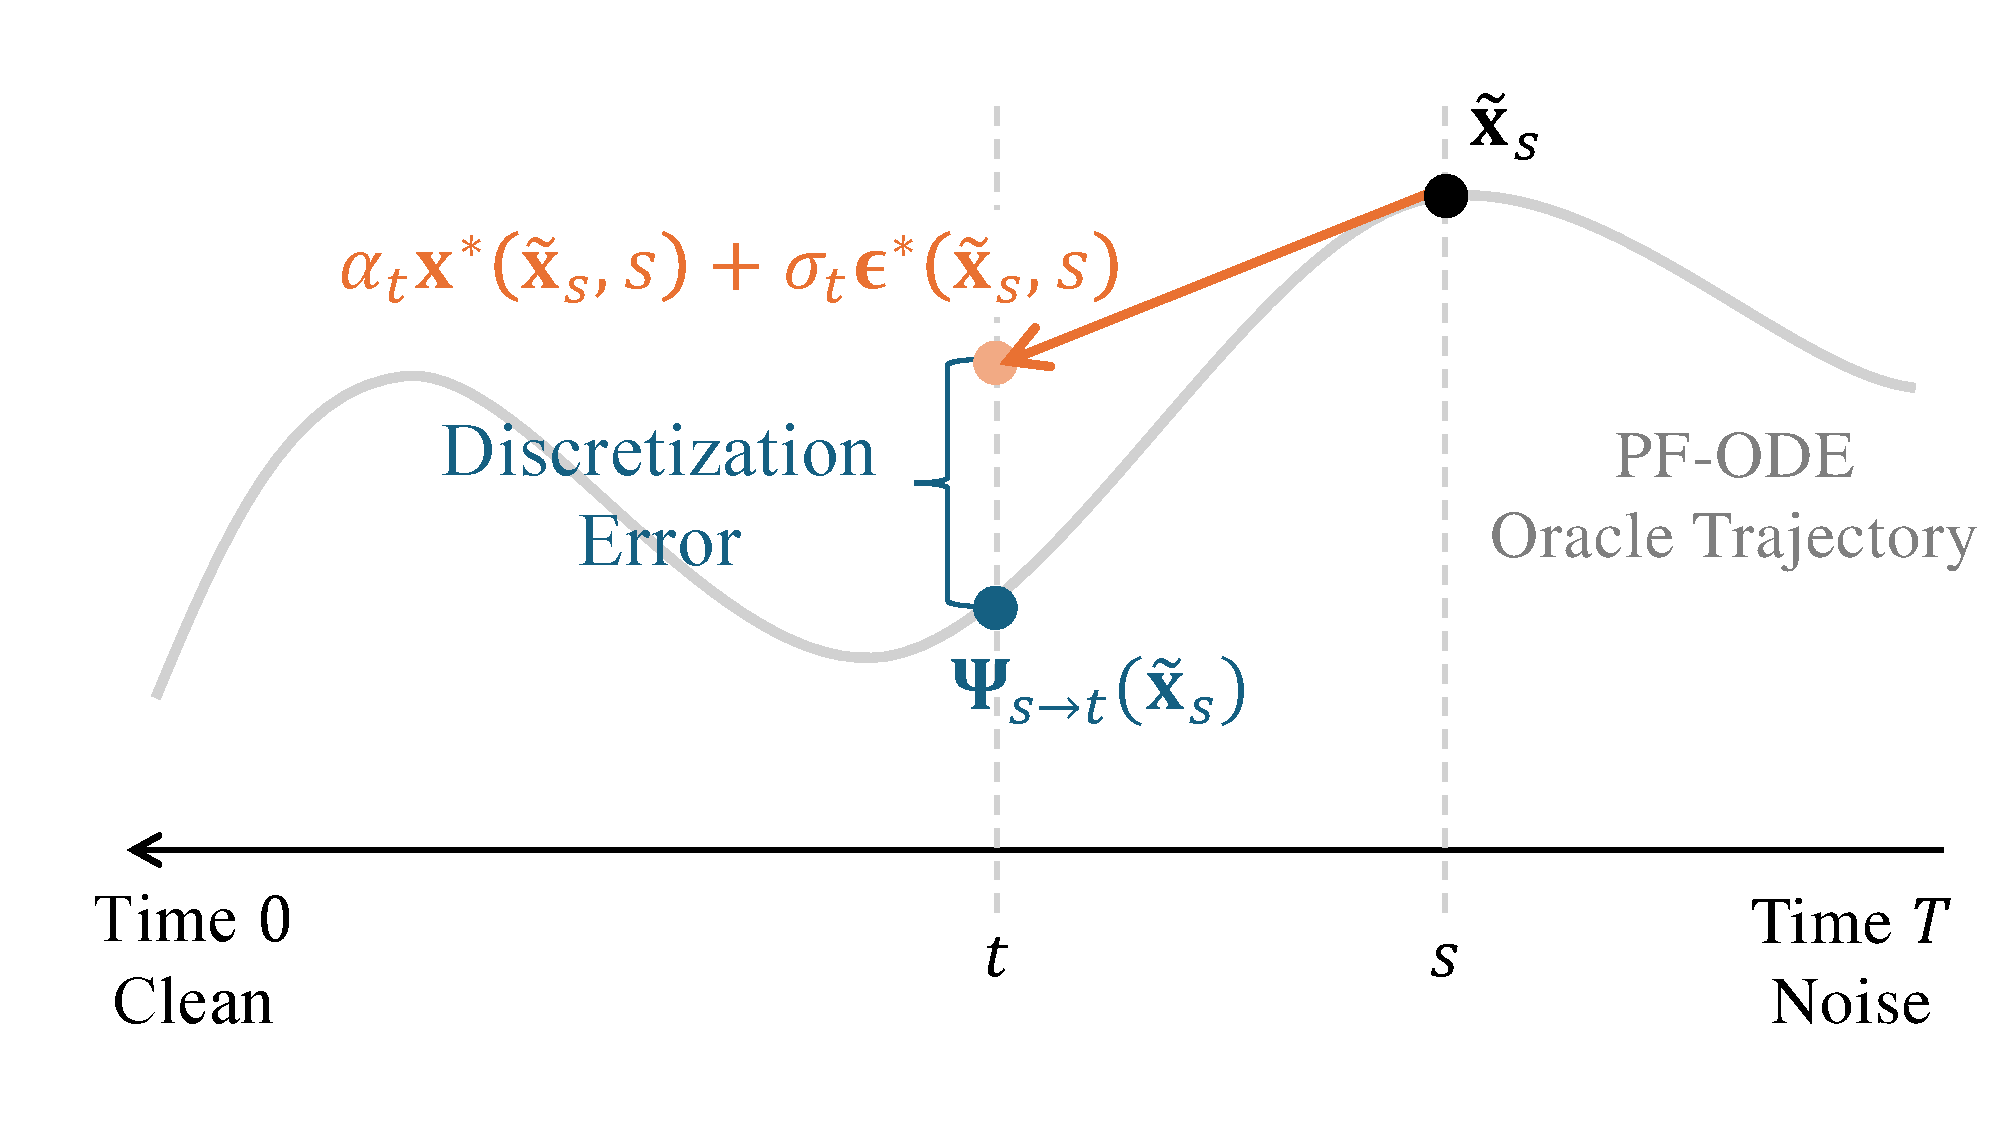
\includegraphics[width=\linewidth]{Images/PartB/Euler.pdf}
    \caption{\textbfs{Illustration of DDIM as an Euler discretization of the PF-ODE.}  Starting from a state $\tilde\rvx_s$ at time $s$, the oracle PF-ODE trajectory (gray curve) deterministically evolves to $\bPsi_{s\to t}(\tilde\rvx_s)$ at time $t$. In contrast, the DDIM update (orange) directly maps $\tilde\rvx_s$ to $\alpha_t \rvx^*(\tilde\rvx_s,s) + \sigma_t \beps^*(\tilde\rvx_s,s)$. The discrepancy between this Euler step and the true PF-ODE trajectory introduces a discretization error, shown in blue. If $t$ is far from $s$, the discrepancy can become large, leading to degraded generation quality.
\figcredit{Created by the authors.}}
    \label{fig:euler}
\end{figure}


With velocity prediction, the linear term $f(t)\rvx$ in the PF-ODE is absorbed into the
target $\rvv^*(\rvx(t), t)=\alpha_t'\rvx_0+\sigma_t'\beps$. By the Fundamental Theorem of Calculus,
the integrals $\int_s^t \alpha_\tau'\diff\tau$ and $\int_s^t \sigma_\tau'\diff\tau$
simplify to $(\alpha_t-\alpha_s)$ and $(\sigma_t-\sigma_s)$, so a single Euler step
already yields the closed-form DDIM update:
\[
\tilde\rvx_t = \alpha_t \tilde\rvx^*(\tilde\rvx_s,s) + \sigma_t \tilde\beps^*(\tilde\rvx_s,s).
\]

That is, with $\rvv$-prediction, there is no separate linear term to isolate in the PF-ODE drift, 
so the plain Euler update naturally coincides with the DDIM formulation.  
In contrast, under the $\beps$-, $\rvx$-, or $\rvs$-prediction parameterizations, 
the PF-ODE drift can be decomposed into a \emph{semilinear} form consisting of a linear term and a nonlinear correction, 
which fits the general template given in \Cref{eq:general-semilinear-pfode}. A naïve Euler step then only \emph{approximates} the linear term instead of computing it exactly 
(see the argument in \Cref{eq:euler-step}). DDIM, on the other hand, corresponds to an \emph{exponential--Euler} (integrating-factor) step 
that handles this linear component analytically.  
Therefore, $\rvv$-prediction leads to the simplest and most direct Euler integration, 
whereas the other parameterizations require the exponential--Euler form to achieve the same DDIM behavior.

The above discussion also echoes the arguments presented in \Cref{subsec:concept-why-v-affine} 
and leads to the following conclusion:
\msg{Observation}{(Exponential) Euler and DDIM Updates}{
Given the same schedulers $(\alpha_t,\sigma_t)$,
\begin{align*}
\text{$\rvv$-prediction:} 
&\quad \text{Euler} = \text{DDIM}, \\[4pt]
\text{$\beps$-, $\rvx$-, or $\rvs$-prediction:} 
&\quad \text{exp--Euler} = \text{DDIM} \neq \text{plain Euler},
\end{align*}
where, in the $\beps$-, $\rvx$-, or $\rvs$-prediction cases, the plain Euler step is not equivalent to DDIM, 
since the linear term is only approximated and may lead to reduced stability.
}





\paragraph{Illustrative Example of DDIM Under Different Parameterizations.}
We illustrate with a simple example using oracle replacements ($\beps^*$, $\rvx^*$, $\nabla_\rvx\log p_t$, and $\rvv^*$), based on \Cref{eq:ddim-update-all}.  
Assume the forward kernel $\alpha_t=1$ and $\sigma_t=t$~\citep{karras2022elucidating}. The DDIM (exp--Euler) update
\[
\tilde\rvx_{t} = \frac{\alpha_{t}}{\alpha_{s}}\tilde\rvx_{s}
- \alpha_{t} \left(\frac{\sigma_{s}}{\alpha_{s}} - \frac{\sigma_{t}}{\alpha_{t}}\right)
\beps^*(\tilde\rvx_{s}, s)
\]
reduces to
\[
\tilde\rvx_t = \tilde\rvx_s - (s-t)\,\beps^*(\tilde\rvx_s,s).
\]
Conceptually, subtracting the time gap $(s-t)$ multiplied by the oracle noise estimate 
$\beps^*(\tilde\rvx_s,s)$ pushes the current sample $\tilde\rvx_s$ toward a cleaner estimate.

Using the $\rvx$-prediction oracle $\rvx^*$, which is related to the noise oracle by
\[
\beps^*(\tilde\rvx_s,s) = \frac{\tilde\rvx_s - \rvx^*(\tilde\rvx_s, s)}{s},
\]
we obtain
\begin{align}\label{eq:ctm-formulation}
    \tilde\rvx_t
 = \tilde\rvx_s - \frac{s-t}{s}\,\bigl(\tilde\rvx_s - \rvx^*(\tilde\rvx_s, s)\bigr)
 = \frac{t}{s}\,\tilde\rvx_s + \Bigl(1-\frac{t}{s}\Bigr)\,\rvx^*(\tilde\rvx_s, s).
\end{align}
Thus, $\tilde\rvx_t$ is a convex combination of the current sample $\tilde\rvx_s$ and the $\rvx$-prediction $\rvx^*(\tilde\rvx_s, s)$, which serves as the oracle estimate of the clean data. Moreover, we can rewrite this as
\[
\tilde\rvx_t-\rvx^* = \frac{t}{s}\,\bigl(\tilde\rvx_s-\rvx^*\bigr),\quad t<s,
\]
which shows that the denoising residual contracts by the factor $t/s\in(0,1)$ at each step (so no overshoot occurs when $t<s$).

Using the score oracle, related to the noise oracle by
\[
\beps^*(\tilde\rvx_s, s) = -\sigma_s \nabla_{\rvx}\log p_s(\tilde\rvx_s),
\]
the DDIM (exp--Euler) update becomes
\[
\tilde\rvx_t = \tilde\rvx_s + (s-t)\,s\,\nabla_{\rvx}\log p_s(\tilde\rvx_s).
\]
This moves $\tilde\rvx_s$ uphill along the score field (toward higher likelihood regions), with step size proportional to the time gap $(s-t)$ and the noise scale $s$.

Finally, using the velocity oracle with $\rvv^*(\tilde\rvx_s,s) = \beps^*(\tilde\rvx_s,s)$, the DDIM update can be written as
\[
\tilde\rvx_t = \tilde\rvx_s + (t-s)\,\rvv^*(\tilde\rvx_s,s),
\]
so the secant slope satisfies the finite-difference identity
\[
\frac{\tilde\rvx_t-\tilde\rvx_s}{t-s} = \rvv^*(\tilde\rvx_s,s).
\]
Intuitively, this means the update is a straight-line step following the local ODE drift.


\paragraph{Challenge of DDIM.}
As a first-order method, DDIM has global discretization error
$\mathcal O(h)$, where $h:=\max_i |t_i-t_{i-1}|$. Accordingly, its
accuracy generally deteriorates as the step size grows. This motivates
higher-order solvers, which use richer local approximations to improve
the global order to $\mathcal O(h^k)$ ($k\ge 2$). With suitable
timestep allocation, such methods may achieve a target quality in fewer
steps. Higher order alone, however, does not guarantee lower wall-clock
cost, since each step may require multiple model evaluations. In
practice, the relevant measure of efficiency is the number of function
evaluations, $\mathrm{NFE}=mN$, so ``faster'' means reaching the desired
quality with a smaller NFE, not merely with fewer steps.

This global $\mathcal O(h)$ statement, while correct, is too coarse to
explain why some PF-ODE trajectories remain well approximated even with
relatively large steps, whereas others do not. A more informative
viewpoint is to ask what quantity DDIM freezes on each step, and how
much that quantity varies along the exact trajectory.

\paragraph{What Actually Controls DDIM's First-Order Error.}
A first important clarification is that the choice of parameterization
does \emph{not} change the exact oracle PF-ODE trajectory. Under the
oracle identities in \Cref{eq:predictions-equivalence}, the
$\rvv$-, $\beps$-, $\rvx$-, and $\rvs$-parameterizations are merely
different representations of the same ODE. What changes is the form in
which the drift is written, and hence which quantity is treated as
approximately constant by the first-order discretization.

\subparagraph{$\rvv$-Prediction Case (DDIM = Euler).}
For $\rvv$-prediction, DDIM is exactly the plain Euler step for
\[
\frac{\diff \rvx(\tau)}{\diff \tau}=\rvv(\rvx(\tau),\tau).
\]
Let $h:=s-t>0$, with $s>t$. Starting from the exact state $\rvx_s$ at
time $s$, the one-step DDIM/Euler update is
\[
\tilde{\rvx}_t^{\mathrm{Euler}}
=
\rvx_s-h\,\rvv(\rvx_s,s).
\]
Taylor's theorem with integral remainder gives
\[
\rvx(t)-\tilde{\rvx}_t^{\mathrm{Euler}}
=
\int_t^s (\tau-t)\,
\frac{\diff}{\diff \tau}\rvv(\rvx(\tau),\tau)\,\diff\tau,
\]
where
\[
\frac{\diff}{\diff \tau}\rvv(\rvx(\tau),\tau)
=
\partial_\tau \rvv(\rvx(\tau),\tau)
+
\nabla_{\rvx}\rvv(\rvx(\tau),\tau)\,\rvv(\rvx(\tau),\tau).
\]
Hence
\[
\|\rvx(t)-\tilde{\rvx}_t^{\mathrm{Euler}}\|
\le
\frac{h^2}{2}\,
\sup_{\tau\in[t,s]}
\Big\|
\partial_\tau \rvv(\rvx(\tau),\tau)
+
\nabla_{\rvx}\rvv(\rvx(\tau),\tau)\,\rvv(\rvx(\tau),\tau)
\Big\|.
\]
Thus, for plain Euler, the relevant quantity is the total time
derivative of the drift evaluated along the exact trajectory,
\[
\frac{\diff}{\diff \tau}\rvv(\rvx(\tau),\tau),
\]
equivalently the trajectory acceleration, which measures how much the
path bends over the step. In particular, if the exact trajectory is
affine in time on $[t,s]$, then Euler is exact on that step. This is a
special property of the underlying oracle trajectory, not a generic
consequence of using $\rvv$-prediction.

\subparagraph{$\beps$-, $\rvx$-, and $\rvs$-Prediction Cases (DDIM = Exp--Euler).}
For $\beps$-, $\rvx$-, and $\rvs$-prediction, DDIM is instead an
exponential--Euler method for the semilinear PF-ODE
\[
\frac{\diff \rvx(\tau)}{\diff \tau}
=
f(\tau)\rvx(\tau)+\rmN(\rvx(\tau),\tau).
\]
Using the variation-of-constants formula,
\[
\rvx(t)
=
\mathcal E(s\shortrightarrow t)\rvx_s
+
\int_s^t
\mathcal E(\tau\shortrightarrow t)\,
\rmN(\rvx(\tau),\tau)\,\diff\tau,
\qquad
\mathcal E(s\shortrightarrow t)
:=
\exp\!\Big(\int_s^t f(u)\,\diff u\Big),
\]
the corresponding exponential--Euler step is
\[
\tilde{\rvx}_t^{\mathrm{Exp}\text{-}\mathrm{Euler}}
=
\mathcal E(s\shortrightarrow t)\rvx_s
+
\left(\int_s^t \mathcal E(\tau\shortrightarrow t)\,\diff\tau\right)
\rmN(\rvx_s,s).
\]
Subtracting the two expressions yields the exact identity
\[
\rvx(t)-\tilde{\rvx}_t^{\mathrm{Exp}\text{-}\mathrm{Euler}}
=
\int_s^t
\mathcal E(\tau\shortrightarrow t)\,
\Big(
\rmN(\rvx(\tau),\tau)-\rmN(\rvx_s,s)
\Big)\,\diff\tau.
\]
Therefore the local error is governed not by the literal straightness of
$\rvx(\tau)$, but by how much the nonlinear residual $\rmN$ varies along
the exact trajectory. If $\mathcal E(\tau\shortrightarrow t)$ is bounded
on $[t,s]$, then
\[
\|\rvx(t)-\tilde{\rvx}_t^{\mathrm{Exp}\text{-}\mathrm{Euler}}\|
\le
\left(\sup_{\tau\in[t,s]}|\mathcal E(\tau\shortrightarrow t)|\right)
\frac{h^2}{2}\,
\sup_{\tau\in[t,s]}
\Big\|
\frac{\diff}{\diff \tau}\rmN(\rvx(\tau),\tau)
\Big\|,
\]
where
\[
\frac{\diff}{\diff \tau}\rmN(\rvx(\tau),\tau)
=
\partial_\tau \rmN(\rvx(\tau),\tau)
+
\nabla_{\rvx}\rmN(\rvx(\tau),\tau)\,
\bigl(f(\tau)\rvx(\tau)+\rmN(\rvx(\tau),\tau)\bigr).
\]
In particular, exponential--Euler is exact on a step whenever
$\rmN(\rvx(\tau),\tau)$ remains constant on that interval.

The main point is therefore not that one parameterization makes the
oracle PF-ODE trajectory ``straight.'' Rather, few-step accuracy is
governed by how little the quantity frozen by the chosen first-order
scheme varies along the exact trajectory: the drift $\rvv$ for plain
Euler, and the nonlinear residual $\rmN$ for exponential--Euler. This
also clarifies why the generic global $\mathcal O(h)$ statement can be
overly coarse in practice. Two trajectories may have very different
few-step behavior even when such worst-case bounds appear similar,
because the actual one-step error is determined by the corresponding
derivatives along the realized oracle path. 

The discussion above
concerns only the discretization error of the numerical solver; in
practice, the total sampling error also includes model mismatch and
approximation error in the learned network.


\subsection{(Optional) A Variational Perspective on DDIM}\label{subsec:ddim}

Indeed, the motivation for DDIM comes from revisiting DDPM through
its variational perspective. In DDPM, the reverse process is tied
to a particular Markovian forward transition kernel
$p(\rvx_t|\rvx_{t-\Delta t})$, which enforces small step sizes in
order to approximate the multi-step posterior correctly. DDIM
departs from this restriction by observing that the training
objective depends only on the marginal perturbations
$p_t(\rvx_t|\rvx_0)$, not on the specific forward transition.
This insight allows one to construct reverse dynamics directly from the
marginals, so intermediate steps can be skipped while marginal consistency is
preserved. Because the transition is defined to map $p_s(\rvx_s|\rvx_0)$ to
$p_t(\rvx_t|\rvx_0)$ for any $t<s$, we may use a coarse time grid with far fewer
updates, which reduces the number of model evaluations and yields fast few-step
sampling.



\paragraph{Revisiting DDPM's Variational View.}
In DDPM, training fixes a family of marginal perturbation kernels
$p_t(\rvx_t|\rvx_0)$ and optimizes a surrogate objective that depends only on these
marginals. At sampling time, however, the reverse conditional is the Bayesian posterior under the one-step forward kernel:
\[
p(\rvx_{t-\Delta t}|\rvx_t,\rvx_0)
= \frac{p(\rvx_t|\rvx_{t-\Delta t})\,p_{t-\Delta t}(\rvx_{t-\Delta t}|\rvx_0)}
       {p_t(\rvx_t|\rvx_0)}.
\]
This ties the reverse update to the \emph{particular} forward transition $p(\rvx_t|\rvx_{t-\Delta t})$.
If one tries to skip steps by enlarging $\Delta t$ while reusing the same one-step kernel, this
no longer matches the true multi-step posterior and typically degrades the marginals.


\paragraph{Original DDIM Motivation.}
DDIM observes that the training objective constrains only the marginals $p_t(\rvx_t|\rvx_0)$, not the
intermediate reverse transitions. Hence, one may \emph{specify} a family of reverse conditionals
${\color{orange}\pi(\rvx_t|\rvx_s,\rvx_0)}$ for any $t<s$ that are \emph{one-step marginally consistent}\footnote{If we choose the ``user-defined'' reverse transition kernel 
$\pi$ in \Cref{eq:ddim-reverse-kernel-def} to be exactly the same as the ``true'' conditional distribution: ${\color{orange}\pi(\rvx_t|\rvx_s,\rvx_0)} = p(\rvx_t|\rvx_s, \rvx_0)$, 
then the marginal consistency condition
   \[
\int {\color{orange}\pi(\rvx_t|\rvx_s,\rvx_0)}\,p_s(\rvx_s|\rvx_0)\diff \rvx_s
= p_t(\rvx_t|\rvx_0)
\] 
is simply the consequence of \emph{law of total probability} (also known as the \emph{tower property}) for the conditional joint distribution:
\[
p_t(\rvx_t|\rvx_0)
= \int p(\rvx_t,\rvx_s|\rvx_0)\diff \rvx_s
= \int p(\rvx_t|\rvx_s,\rvx_0)\,p_s(\rvx_s|\rvx_0)\diff \rvx_s.
\]
Or equivalently, by explicitly expressing the Bayesian posterior as
\[
p(\rvx_t|\rvx_s,\rvx_0)
= \frac{p(\rvx_s|\rvx_t,\rvx_0)\,p_t(\rvx_t|\rvx_0)}
       {p_s(\rvx_s|\rvx_0)},
\]
then multiplying by $p_s(\rvx_s|\rvx_0)$ and marginalizing over $\rvx_s$, we
recover
\[
\int p(\rvx_t|\rvx_s,\rvx_0)\,p_s(\rvx_s|\rvx_0) \diff \rvx_s
= p_t(\rvx_t|\rvx_0),
\]
which is exactly the same marginal-consistency condition.

In the Markov forward case, one further has 
$p(\rvx_t|\rvx_s,\rvx_0)=p(\rvx_t|\rvx_s)$, 
reducing the following expression:
\[
p_t(\rvx_t|\rvx_0)
= \int p(\rvx_t|\rvx_s)\,p_s(\rvx_s|\rvx_0)\diff \rvx_s.
\]
}:
\begin{mdframed}
    \begin{align}\label{eq:ddim-reverse-kernel-def}
\int {\color{orange}\pi(\rvx_t|\rvx_s,\rvx_0)}\,p_s(\rvx_s|\rvx_0) \diff \rvx_s
= p_t(\rvx_t|\rvx_0).
\end{align}
\end{mdframed}
This construction removes any dependence on the forward one-step kernel $p(\rvx_t|\rvx_{t-\Delta t})$
and legitimizes coarse (skipped) time steps. 

\paragraph{Derivation of Discrete-Time DDIM.}
Consider the general forward perturbation:
\begin{equation*}
    p_t(\rvx_t|\rvx_0) := \mathcal{N}\big(\rvx_t; \alpha_t \rvx_0, \sigma_t^2 \mathbf{I}\big),
\end{equation*}
where $\rvx_0 \sim p_{\mathrm{data}}$. 


DDIM does not require the reverse update to coincide with the Bayesian posterior tied to the
one-step forward kernel. It suffices to \emph{choose} a reverse conditional that preserves the
marginals. Concretely, for any $t<s$ we posit the Gaussian family
\begin{align}\label{eq:ddim-reverse-kernel-param}
{\color{orange}\pi(\rvx_t|\rvx_s,\rvx_0)}
= \mathcal{N} \big(\rvx_t;\, a_{t,s}\,\rvx_0 + b_{t,s}\,\rvx_s,\; c_{t,s}^2\,\mathbf{I}\big),
\end{align}
with coefficients $(a_{t,s},b_{t,s},c_{t,s})$ to be determined by the marginal-consistency
constraint \Cref{eq:ddim-reverse-kernel-def}. Since all involved kernels are Gaussian, sampling
$\rvx_s|\rvx_0=\alpha_s\rvx_0+\sigma_s\beps'$ and then
$\rvx_t|\rvx_s,\rvx_0$ from \Cref{eq:ddim-reverse-kernel-param} yields
\begin{align}\label{eq:ddim-derivation} 
\begin{aligned}
\rvx_t
&= a_{t,s}\,\rvx_0 + b_{t,s}\,\rvx_s + c_{t,s}\,\beps
\\&= a_{t,s}\,\rvx_0 + b_{t,s}\big(\alpha_s\rvx_0+\sigma_s\beps'\big) + c_{t,s}\,\beps \\
&= (a_{t,s} + b_{t,s}\alpha_s)\,\rvx_0
+ \sqrt{b_{t,s}^2\sigma_s^2 + c_{t,s}^2}\;\beps'',
\end{aligned}
\end{align}
where $\beps,\beps',\beps''\sim\mathcal{N}(\mathbf{0},\mathbf{I})$ are independent (Gaussian-sum
property). On the other hand,
\[
\rvx_t\sim p_t(\rvx_t|\rvx_0)
= \mathcal{N} \big(\rvx_t; \alpha_t\rvx_0, \sigma_t^2\mathbf{I}\big).
\]
Equating means and variances between this target and \Cref{eq:ddim-derivation} gives
\begin{align*}
\alpha_t = a_{t,s} + b_{t,s}\alpha_s,
\qquad
\sigma_t^2 = b_{t,s}^2\sigma_s^2 + c_{t,s}^2.
\end{align*}
This system is underdetermined, so we treat $c_{t,s}$ as a free parameter with the natural constraint
$0\le c_{t,s} \le \sigma_t$, and solve for $a_{t,s},b_{t,s}$:
\begin{align}\label{eq:ddim-coefficients}
b_{t,s} = \frac{\sqrt{\sigma_t^2 - c_{t,s}^2}}{\sigma_s},
\qquad
a_{t,s} = \alpha_t - \alpha_s\,b_{t,s}.
\end{align}
Here, we take the nonnegative root for $b_{t,s}$ without loss of generality.

Substituting \Cref{eq:ddim-coefficients} into \Cref{eq:ddim-reverse-kernel-param} yields
\begin{align}\label{eq:ddim-reverse-kernel-result}
{\color{orange}\pi(\rvx_t|\rvx_s,\rvx_0)}
= \mathcal{N} \Big(
\rvx_t;\;
\underbrace{\alpha_t\rvx_0
+ \frac{\sqrt{\sigma_t^2 - c_{t,s}^2}}{\sigma_s}\,(\rvx_s - \alpha_s\rvx_0)}_{\text{mean}},
\;\; c_{t,s}^2\mathbf{I}\Big).
\end{align}
Equivalently, the mean in \Cref{eq:ddim-reverse-kernel-result} expands to
\[
\Big(\alpha_t - \alpha_s\frac{\sqrt{\sigma_t^2 - c_{t,s}^2}}{\sigma_s}\Big)\rvx_0
+ \Big(\frac{\sqrt{\sigma_t^2 - c_{t,s}^2}}{\sigma_s}\Big)\rvx_s.
\]

\lem{DDIM Coefficients}{ddim-coeff}{
Let ${\color{orange}\pi(\rvx_t|\rvx_s,\rvx_0)}$ be given by \Cref{eq:ddim-reverse-kernel-param}.
If the marginal-consistency condition \Cref{eq:ddim-reverse-kernel-def} holds, then the coefficients
are exactly those in \Cref{eq:ddim-coefficients}, with $0\le c_{t,s}\le \sigma_t$.
}

\rmkb{
\begin{enumerate}[leftmargin=*]
    \item In DDIM we \emph{choose} the reverse kernel ${\color{orange}\pi(\rvx_t|\rvx_s,\rvx_0)}$ to satisfy the
marginal-consistency constraint, and in general 
\[
{\color{orange}\pi(\rvx_t|\rvx_s,\rvx_0)}\neq p (\rvx_t|\rvx_s,\rvx_0),
\]
where $p (\rvx_t|\rvx_s,\rvx_0)$ is the Bayesian posterior associated with a particular forward
one-step kernel. By Bayes’ rule,
\[
p(\rvx_t|\rvx_s,\rvx_0)\;\propto\; p(\rvx_s|\rvx_t)\,p_t(\rvx_t|\rvx_0),
\]
and this posterior is \emph{not} required for specifying $\pi$ or for training.
    \item Only in the special case where the variance parameter is chosen to match the DDPM posterior
variance (the $\eta=1$ setting in \Cref{eq:eta-ddim}) do we have ${\color{orange}\pi(\rvx_t|\rvx_s,\rvx_0)}=
p (\rvx_t|\rvx_s,\rvx_0)$; otherwise ${\color{orange}\pi(\rvx_t|\rvx_s,\rvx_0)} \neq
p (\rvx_t|\rvx_s,\rvx_0)$.
    \item Without imposing a Markov constraint, in general $p(\rvx_s|\rvx_t,\rvx_0)\neq p(\rvx_s|\rvx_t)$.
The equality $p(\rvx_s|\rvx_t,\rvx_0)=p(\rvx_s|\rvx_t)$ is tied to a particular Markov forward model,
which DDIM does not assume for its reverse construction.
\end{enumerate}
}


The forward marginals $\{p_t(\rvx_t|\rvx_0)\}_t$ do not uniquely determine the reverse conditional
transitions. There exist infinitely many kernels
${\color{orange}\pi(\rvx_t|\rvx_s,\rvx_0)}$ that satisfy
\Cref{eq:ddim-reverse-kernel-def}, any of which can be freely specified.
The parameter $c_{t,s}$ indexes this family and controls the amount of noise injected
at each reverse step $s \to t$. Below, we introduce this family of DDIM solvers.




\paragraph{DDIM Sampler (Step $s\to t$).}
The DDIM sampler follows from the chosen reverse kernel ${\color{orange}\pi(\rvx_t|\rvx_s,\rvx_0)}$ in
\Cref{eq:ddim-reverse-kernel-result} by replacing $\rvx_0$ with a predictor from a pre-trained model.
Using the $\beps$-prediction network $\beps_{\bm{\phi}^\times}$ (plug-and-play, no retraining), we set
\[
\rvx_{\bm{\phi}^\times}(\rvx_s,s)
:= \frac{\rvx_s - \sigma_s\,\beps_{\bm{\phi}^\times}(\rvx_s,s)}{\alpha_s},
\quad
p_{\bm{\phi}^\times}(\rvx_t|\rvx_s)
:= {\color{orange}\pi\big(\rvx_t\,\big|\,\rvx_s,\rvx_{\bm{\phi}^\times}(\rvx_s,s)\big)}.
\]
Substituting $\rvx_{\bm{\phi}^\times}$ into \Cref{eq:ddim-reverse-kernel-result} yields the update
\begin{mdframed}
\[
\rvx_t
= \frac{\alpha_t}{\alpha_s}\,\rvx_s
+\Big(\sqrt{\sigma_t^2 - c_{t,s}^2}-\frac{\alpha_t}{\alpha_s}\sigma_s\Big)\,
\beps_{\bm{\phi}^\times}(\rvx_s,s)
+ c_{t,s}\,\beps_t,
\quad \beps_t\sim\mathcal{N}(\mathbf{0},\mathbf{I}),
\]
\end{mdframed}
where $c_{t,s}\in[0,\sigma_t]$ controls stochasticity.

For notational convenience define the forward factors
\[
\alpha_{t|s}:=\tfrac{\alpha_t}{\alpha_s},
\qquad
\sigma_{t|s}^2:=\sigma_t^2-\alpha_{t|s}^2\,\sigma_s^2,
\]
so that $p(\rvx_t|\rvx_s)=\mathcal{N}(\alpha_{t|s}\rvx_s,\sigma_{t|s}^2\mathbf{I})$. Then the sampler can be written as
\[
\rvx_t
= \alpha_{t|s}\,\rvx_s
+\big(\sqrt{\sigma_t^2 - c_{t,s}^2}-\alpha_{t|s}\sigma_s\big)\,
\beps_{\bm{\phi}^\times}(\rvx_s,s)
+ c_{t,s}\,\beps_t.
\]

By varying $c_{t,s}$, one obtains a family of samplers that share the same pre-trained diffusion model and do not require retraining:
\begin{itemize}
\item \textbfs{DDPM Step (Posterior Variance):}
$
c_{t,s}=\frac{\sigma_s}{\sigma_t}\,\sigma_{t|s}
$
makes ${\color{orange}\pi(\rvx_t|\rvx_s,\rvx_0)}$ equal to the Bayesian posterior
$p(\rvx_t|\rvx_s,\rvx_0)$ induced by the one-step forward kernel.
Replacing $\rvx_0$ with its predictor yields the standard DDPM reverse update
$p_{\bm{\phi}^\times}(\rvx_t|\rvx_s)$, i.e., the Markov DDPM step with $\alpha_t^2+\sigma_t^2=1$ (\Cref{eq:ddpm-sampling}).

\item \textbfs{Deterministic DDIM ($\eta=0$):}
$
c_{t,s}=0
$
gives
\[
\rvx_t
= \alpha_{t|s}\rvx_s + \big(\sigma_t-\alpha_{t|s}\sigma_s\big)\beps_{\bm{\phi}^\times}(\rvx_s,s),
\]
which matches the ODE-view DDIM jump.

\item \textbfs{Interpolation:} Define
\begin{align}\label{eq:eta-ddim}
    c_{t,s}=\eta\,\frac{\sigma_s}{\sigma_t}\,\sigma_{t|s}, \quad \eta\in[0,1],
\end{align}
so that $\eta$ smoothly interpolates between the stochastic DDPM update ($\eta=1$) and the deterministic DDIM update ($\eta=0$).
\end{itemize}





\subsection{DDIM as Conditional Flow Matching}\label{subsec:ddim-cfm}
In this subsection, we will see that deterministic DDIM can be understood as searching for a conditional flow map that pushes $p_s(\cdot|\rvx_0)$ forward to $p_t(\cdot|\rvx_0)$.  
The tangent of this conditional flow coincides with the conditional velocity used in conditional flow matching (CFM).  
Marginalizing this conditional velocity yields the PF–ODE drift, whose plain Euler discretization recovers the marginal DDIM update in $\rvv$-prediction.

We revisit the DDIM one–step conditional marginal–consistency identity (\Cref{eq:ddim-reverse-kernel-def})
\[
\int {\color{orange}\pi(\rvx_t|\rvx_s,\rvx_0)} p_s(\rvx_s|\rvx_0) \diff \rvx_s
= p_t(\rvx_t|\rvx_0), \quad t<s,
\]
i.e., if $\rvx_s\sim p_s(\cdot|\rvx_0)$ then pushing $\rvx_s$ forward by the chosen reverse kernel reproduces $p_t(\cdot|\rvx_0)$.  
When the reverse kernel is deterministic, it amounts to finding a conditional map 
$\bPsi_{s\to t}(\cdot|\rvx_0)$ that pushes $p_s(\cdot|\rvx_0)$ forward to $p_t(\cdot|\rvx_0)$:
\[
{\color{orange}\pi(\rvx_t|\rvx_s,\rvx_0)}
=\delta \big(\rvx_t-\bPsi_{s\to t}(\rvx_s|\rvx_0)\big),
\qquad
\bigl(\bPsi_{s\to t}(\cdot|\rvx_0)\bigr)_{\#}p_s(\cdot|\rvx_0)=p_t(\cdot|\rvx_0).
\]


Under the linear–Gaussian path $\rvx_\tau=\alpha_\tau\rvx_0+\sigma_\tau\beps$, 
similar arguments as in \Cref{eq:ddim-reverse-kernel-param,eq:ddim-derivation} 
lead to the \textit{conditional map}
\[
\bPsi_{s\to t}(\rvx_s|\rvx_0)
=\frac{\sigma_t}{\sigma_s}\,\rvx_s
+\Bigl(\alpha_t-\alpha_s\frac{\sigma_t}{\sigma_s}\Bigr)\rvx_0,
\]
whose instantaneous \textit{conditional velocity} is
\[
\rvv_t^{*}(\rvx|\rvx_0)
=\partial_h \big|_{h=0}\bPsi_{t\to t+h}(\rvx|\rvx_0)
=\frac{\sigma_t'}{\sigma_t}\,\rvx
+\Bigl(\alpha_t'-\alpha_t\frac{\sigma_t'}{\sigma_t}\Bigr)\rvx_0.
\]
We refer to $\bPsi_{s\to t}(\cdot|\rvx_0)$ as the DDIM conditional map.

With $p_t(\rvx|\rvx_0)$, conditional flow matching fits the time–dependent field to this target velocity,
\[
\mathcal L_{\mathrm{CFM}}(\bphi)
=\E_{t,\rvx_0,\rvx_t\sim p_t(\cdot|\rvx_0)}
\big\|\rvv_\bphi(\rvx_t,t)-\rvv_t^{*}(\rvx_t|\rvx_0)\big\|^2,
\]
so the CFM regression target equals the conditional velocity of the DDIM conditional map.

\msg{Observation}{Conditional Level}{
Along the conditional Gaussian path, the DDIM conditional map and the CFM target generate the same conditional flow $\bPsi_{s\to t}(\cdot|\rvx_0)$.
}

Averaging the conditional velocity over the posterior of $\rvx_0$ given $\rvx_t=\rvx$ yields the marginal PF–ODE drift,
\[
\rvv^*(\rvx,t)=\E \left[\rvv_t^*(\rvx| \rvx_0)|\rvx_t=\rvx\right],
\]
which, under the linear–Gaussian scheduler, takes the separable predictor form
\[
\rvv^*(\rvx,t)=\alpha_t'\,\rvx^*(\rvx,t)+\sigma_t'\,\beps^*(\rvx,t),
\quad
\rvx=\alpha_t\,\rvx^*(\rvx,t)+\sigma_t\,\beps^*(\rvx,t).
\]
We have seen that the plain Euler step of the PF-ODE with this marginalized $\rvv$–prediction is exactly the DDIM  update (the last identity in \Cref{eq:ddim-update-all}).

In short, DDIM is (i) a deterministic conditional transport whose tangent equals the CFM target, and (ii) after marginalizing that tangent, a Euler step of the PF–ODE whose step coincides with the DDIM update.


\newpage

% \paragraph{(Optional, move to appendix) Gauge freedom and rotations}
% More generally, one may replace the shared-noise coupling with any orthogonal transformation
% $\rmR_{s\to t}\in\mathrm{O}(D)$, yielding
% \[
% \rmT^{\rvx_0}_{s\to t}(\rvx_s)
% =\frac{\sigma_t}{\sigma_s}\,\rmR_{s\to t}\,\rvx_s
% +\Big(\alpha_t-\alpha_s\frac{\sigma_t}{\sigma_s}\,\rmR_{s\to t}\Big)\rvx_0,
% \qquad
% \beps_t=\rmR_{s\to t}\beps_s.
% \]
% Each such choice preserves the marginal consistency condition, introducing a \emph{gauge freedom} in the noise rotation.
% For the maps to compose consistently across time, the rotations must satisfy the cocycle (semigroup) rule
% \[
% \rmR_{s\to t}=\rmR_{u\to t}\,\rmR_{s\to u},\qquad
% \rmR_{t\to t}=\rmI.
% \]
% DDIM corresponds to the simplest gauge, $\rmR_{s\to t}=\rmI$, where all noise directions are aligned (shared across time).
% Since this specific gauge already yields the standard DDIM flow and serves as the target for CFM,
% the broader rotation family is optional and mainly of theoretical interest.


%%%%%%%%%%%%%%%%%%%%%%%%%%%%
% In this subsection, we further focus on the discussion on the (variational perspective) DDIM marginal-consistency identity (\Cref{eq:ddim-reverse-kernel-def})
% \begin{align*}
% \int {\color{orange}\pi(\rvx_t|\rvx_s,\rvx_0)}p_s(\rvx_s|\rvx_0)\diff \rvx_s
% = p_t(\rvx_t|\rvx_0), \quad t<s.
% \end{align*}
% It states that, if $\rvx_s\sim p_s(\cdot|\rvx_0)$, then pushing $\rvx_s$ forward by the
% user-specified kernel ${\color{orange}\pi(\cdot|\rvx_s,\rvx_0)}$ produces the correct later marginal
% $p_t(\cdot|\rvx_0)$.


% \paragraph{Deterministic Kernels $\Rightarrow$ Pushforward Maps.}
% When the reverse kernel ${\color{orange}\pi(\rvx_t|\rvx_s,\rvx_0)}$ is chosen to be \emph{deterministic}, it can be written as a Dirac measure
% concentrated at the output of a conditional map $\rmT^{\rvx_0}_{s\to t}$:
% \[
% {\color{orange}\pi(\rvx_t|\rvx_s,\rvx_0)}
% = \delta \big(\rvx_t-\rmT^{\rvx_0}_{s\to t}(\rvx_s)\big),
% \]
% Here, $\rmT^{\rvx_0}_{s\to t}(\cdot):\R^D \to \R^D$ is a function that evolves the state from time $s$ to time $t$ given a endpoint $\rvx_0$.

% In this case, one-step marginal consistency becomes searching a conditional (on $\rvx_0$) deterministic map $\rmT^{\rvx_0}_{s\to t}$ that satisfies the  pushforward relation
% \[
% (\rmT^{\rvx_0}_{s\to t})_{\#}\,p_s(\cdot|\rvx_0)=p_t(\cdot|\rvx_0).
% \]

% \paragraph{Gaussian Forward and the General Form of a Marginal-Correct Map.}
% Assume the standard linear–Gaussian forward conditionals
% \[
% p_\tau(\rvx_\tau|\rvx_0)=\mathcal N \big(\rvx_\tau;\alpha_\tau \rvx_0,\;\sigma_\tau^2 \rmI\big),\qquad \sigma_\tau>0.
% \]
% If a deterministic map pushes $p_s(\cdot|\rvx_0)$ to $p_t(\cdot|\rvx_0)$ for \emph{all} $\rvx_0$, then (classically) it must be
% \emph{affine}:
% \[
% \rmT^{\rvx_0}_{s\to t}(\rvx_s)=\rmA_{s\to t}\rvx_0 + \rmB_{s\to t}\rvx_s,
% \]
% and matching the Gaussian mean and covariance forces
% \[
% \rmA_{s\to t}=\alpha_t\rmI-\alpha_s\frac{\sigma_t}{\sigma_s}\rmR_{s\to t},\quad 
% \rmB_{s\to t}=\frac{\sigma_t}{\sigma_s}\rmR_{s\to t}
% \]
% where $\rmR_{s\to t}$ is any $D\times D$ orthogonal matrix.
% Hence the more general deterministic, marginal-correct update (oracle case) is
% \[
% \rmT^{\rvx_0}_{s\to t}(\rvx_s)
% =\frac{\sigma_t}{\sigma_s}\rmR_{s\to t}\,\rvx_s
% +\Big(\alpha_t-\alpha_s\frac{\sigma_t}{\sigma_s}\rmR_{s\to t}\Big)\rvx_0.
% \]
% The orthogonal factor $\rmR_{s\to t}$ is a genuine \emph{gauge freedom}: it does not change the one-step marginals.


% \paragraph{Route to Standard DDIM.}
% For any fixed $\rvx_0$, if the family $\{\rmT^{\rvx_0}_{s\to t}(\cdot)\}_{s,t}$ is continuous in $t$,
% locally Lipschitz in $\rvx$, and satisfies $\rmT^{\rvx_0}_{t\to t}=\mathrm{Id}$, then it constitutes the
% \emph{conditional flow map} (evolution family) of an ODE. We write this conditional flow map as $ \bPsi_{s\to t}(\cdot|\rvx_0)$ to replace $\rmT^{\rvx_0}_{s\to t}(\cdot)$. Its conditional velocity is derived (?) defined (?) in the following sense: by taking time differentiation:
% \[
% \rvv_t(\rvx|\rvx_0):= \lim_{h\to 0}\frac{\big(\bPsi_{t\to t+h}(\rvx|\rvx_0)-\rvx\big)}{h}, \quad\text{for any }\, t
% \]
% whenever the limit exists. Standard existence and uniqueness results for ODEs then ensure that this conditional
% vector field generates the given  conditional flow (i.e., the  continuity equation is fulfilled). 

% Since $ \bPsi_{s\to t}(\cdot|\rvx_0)$ is an ODE flow map, the following holds automatically by uniqueness, which is known as \emph{semigroup property} for flow maps:
% \[
% \bPsi_{s\to t}(\cdot|\rvx_0)=\bPsi_{u\to t}(\cdot|\rvx_0) \circ \bPsi_{s\to u}(\cdot|\rvx_0),
% \quad
% \bPsi_{t\to t}(\cdot|\rvx_0)=\mathrm{Id}.
% \]
% This implies the rotation matrix (gauge freedom) $\rmR_{s\to t}$ needs to satisfies: 
% \[
% \rmR_{s\to t} = \rmR_{u\to t} \circ \rmR_{s\to u},
% \]
% while there are infinitely many choices for this rotation matrix.

% In the standard DDIM, condition on $\rvx_0$ and pick the path $\rvx_t=\alpha_t \rvx_0+\sigma_t\beps$ with \emph{shared} $\beps$. It fixes the gauge freedom by the \emph{shared-noise}  $\beps\sim \mathcal{N}(\bm{0}, \rmI)$ choice:
% \[
% \beps_t=\beps_s=\beps,\quad \text{for any }\, s>t.
% \]
% This is equivalent to enforcing   $\rmR_{s\to t}=\rmI$ for all $s>t$. 

% With this shared noise, it leads to the standard DDIM deterministic update:
% \[
% \bPsi_{s\to t}(\rvx_s| \rvx_0)
% =\frac{\sigma_t}{\sigma_s}\,\rvx_s+\Big(\alpha_t-\alpha_s\frac{\sigma_t}{\sigma_s}\Big)\rvx_0.
% \]


% \paragraph{How this Connects to Flow Matching.}

% Its time derivative gives a \emph{conditional velocity}
% \[
% \rvv_t(\rvx| \rvx_0)=\alpha_t' \rvx_0+\frac{\sigma_t'}{\sigma_t}\big(\rvx-\alpha_t\rvx_0\big).
% \]
% \emph{Conditional Flow Matching} trains a model to match this drift; integrating it recovers the DDIM map above.
% Unconditioning (averaging over $\rvx_0$ given $\rvx_t$) yields the familiar probability-flow ODE drift used in score-based samplers.

% \paragraph{Practical note.}
% At sampling time, $\rvx_0$ is unknown and replaced by a denoiser  $\rvx_{\bphi^\times}(\rvx_s,s)$, so both one-step marginal matching and semigroup hold only \emph{approximately}. Enforcing composition (CK/semigroup) during design or training can improve robustness to step size, but the core DDIM update follows already from one-step marginals plus the shared-noise gauge.


%%%%%%%%%%%%%%%%%%%%%%%%%%%%%
% \paragraph{(Optional) Chapman--Kolmogorov Identity vs.\ Semigroup Property.}
% Important: the pushforward relationship does not force different time pairs to be compatible. You can satisfy all pairs $(s,t)$ and still have
% $\rmT^{\rvx_0}_{t\to u} \circ \rmT^{\rvx_0}_{s\to t}\neq \rmT^{\rvx_0}_{s\to u}$.


% The Chapman--Kolmogorov (CK) identity composes kernels across an intermediate time:
% \[
% \pi_{s\to u}(\rvx_u|\rvx_s,\rvx_0)
% =\int \pi_{t\to u}(\rvx_u|\rvx_t,\rvx_0)\,\pi_{s\to t}(\rvx_t|\rvx_s,\rvx_0)\diff\rvx_t\quad(s>t>u).
% \]
% In the deterministic case this reduces to the \emph{semigroup property} for maps
% \[
% \rmT^{\rvx_0}_{s\to u}=\rmT^{\rvx_0}_{t\to u}\circ \rmT^{\rvx_0}_{s\to t},
% \qquad
% \rmT^{\rvx_0}_{t\to t}=\mathrm{Id}.
% \]
% CK/semigroup is strictly \emph{stronger} than one-step marginal consistency.



%%%%%%%%%%%%%%%%%%%%%%%%%%


% ---------
% DDIM relaxes the Markovian assumption in the reverse (inference) process to enable fast sampling; defining the reverse transitions as Markovian is unnecessary. Instead, infinitely many choices exist for
% $p(\rvx_{t-\Delta t}|\rvx_t, \rvx_0)$ (i.e., there are infinitely many valid reverse transition distributions that map from $\mathbf{x}_t$ to $\mathbf{x}_{t-\Delta t}$ given $\mathbf{x}_0$), as long as the marginal consistency condition is satisfied:
% \begin{align}\label{eq:marginal_ddim}
%     \int p(\rvx_{t-\Delta t}|\rvx_t, \rvx_0)   p_t(\rvx_t|\rvx_0)   \diff\rvx_t = p_{t-\Delta t}(\rvx_{t-\Delta t}|\rvx_0).
% \end{align}

% We assume that $p(\rvx_{t-\Delta t}|\rvx_t, \rvx_0)$ is Gaussian, which is natural given the Gaussian forward kernels, and take it in the form:
% \begin{align}\label{eq:ddim-reverse-kernel-def}
%     p(\rvx_{t-\Delta t}|\rvx_t, \rvx_0) := \mathcal{N}\big(\rvx_{t-\Delta t}; a_t \rvx_0 + b_t \rvx_t, c_t^2 \mathbf{I}\big),
% \end{align}
% where coefficients $a_t, b_t, c_t$ are to be determined by \Cref{eq:marginal_ddim}. Since all involved kernels are Gaussian, the marginal consistency condition expands to
% \begin{align}\label{eq:ddim-derivation}
% \begin{aligned}
%     \rvx_{t-\Delta t} 
%     &= a_t \rvx_0 + b_t \rvx_t + c_t \bm{\epsilon} \\
%     &= a_t \rvx_0 + b_t (\alpha_t \rvx_0 + \sigma_t \bm{\epsilon}') + c_t \bm{\epsilon} \\
%     &= (a_t + b_t \alpha_t) \rvx_0 + \sqrt{(b_t \sigma_t)^2 + c_t^2} \bm{\epsilon}'',
% \end{aligned}
% \end{align}
% where $\bm{\epsilon}, \bm{\epsilon}', \bm{\epsilon}'' \sim \mathcal{N}(\bm{0}, \mathbf{I})$ are independent and we used the Gaussian sum property.

% On the other hand, from the forward process,
% \[
% \rvx_{t-\Delta t} \sim p_{t-\Delta t}(\rvx_{t-\Delta t}|\rvx_0) = \mathcal{N}\big(\rvx_{t-\Delta t}; \alpha_{t-\Delta t} \rvx_0, \sigma_{t-\Delta t}^2 \mathbf{I}\big),
% \]
% so equating means and variances in \Cref{eq:ddim-derivation} yields
% \begin{align}
% \begin{cases}
%     \alpha_{t-\Delta t} = a_t + b_t \alpha_t, \\
%     \sigma_{t-\Delta t} = \sqrt{(b_t \sigma_t)^2 + c_t^2}.
% \end{cases}
% \end{align}
% Since this system is underdetermined (i.e., has infinitely many solutions), we can treat $c_t$ as a free parameter and solve for $a_t$ and $b_t$, summarizing the result in the following lemma.
% \lem{DDIM Coefficients}{ddim-coeff}{
% Define the reverse conditional kernel as in \Cref{eq:ddim-reverse-kernel-def} with coefficients $a_t, b_t, c_t$. If it satisfies the marginal condition \Cref{eq:marginal_ddim}, then
% \begin{align*}
%     a_t &= \alpha_{t-\Delta t} - \alpha_t \frac{\sqrt{\sigma_{t-\Delta t}^2 - c_t^2}}{\sigma_t}, \quad
%     b_t = \frac{\sqrt{\sigma_{t-\Delta t}^2 - c_t^2}}{\sigma_t}.
% \end{align*}
% }
% Hence,
% \begin{align}\label{eq:ddim-reverse-kernel-result}
% \begin{aligned}
%     p(\rvx_{t-\Delta t}|\rvx_t, \rvx_0) = \mathcal{N}\Bigg(&
%         \rvx_{t-\Delta t}; 
%         \left(\alpha_{t-\Delta t} - \alpha_t \frac{\sqrt{\sigma_{t-\Delta t}^2 - c_t^2}}{\sigma_t}\right) \rvx_0 \\
%         &\quad+ \left(\frac{\sqrt{\sigma_{t-\Delta t}^2 - c_t^2}}{\sigma_t}\right) \rvx_t,
%         c_t^2 \mathbf{I}
%     \Bigg).
% \end{aligned}
% \end{align}
% \rmkb{
% Note that in the DDIM setup, in general,
% \[
% p(\rvx_t|\rvx_{t-\Delta t}, \rvx_0) \neq p(\rvx_t|\rvx_{t-\Delta t}),
% \]
% since the Markov assumption is not imposed. An analogous identity from Bayes' rule states that
% \[
% p(\rvx_{t-\Delta t}|\rvx_t, \rvx_0) = p(\rvx_t|\rvx_{t-\Delta t}, \rvx_0) \frac{p_{t-\Delta t}(\rvx_{t-\Delta t}|\rvx_0)}{p_t(\rvx_t|\rvx_0)}.
% \]
% Although we can compute $p(\rvx_t|\rvx_{t-\Delta t}, \rvx_0)$ using this identity, it is generally not used for training or sampling.\dk{Isn't it used to derive Eq. (2.2.3)? Other than thsi Bayes rule, how could we derive the loss function?}
% }
% Until now, we emphasize the key insight behind the DDIM approach from a variational perspective:
% \msg{Insight}{}{
% The forward marginal distributions $\{p_t(\rvx_t|\rvx_0)\}_t$ alone do not uniquely determine the reverse conditional transitions; in fact, there are infinitely many $p(\rvx_{t-\Delta t}|\rvx_t, \rvx_0)$ satisfying the marginal consistency (e.g., parameterized by $c_t$).
% }



% \paragraph{Discrete-Time DDIM Sampler.}  
% The key difference between DDIM and the formulation in DDPM (\Cref{sec:variational-perspective}) lies in modeling the conditional distribution $p(\rvx_{t-\Delta t}|\rvx_t, \rvx_0)$. Thus, DDIM enables a plug-and-play approach\footnote{See Theorem 1 in \citep{song2020denoising}.} to leverage any pre-trained diffusion model without retraining. 

% Here, we adapt the $\beps$-prediction model $\bm{\epsilon}_{\bm{\phi}^\times}$ as in the original DDPM, which can be easily converted to clean or other prediction forms via \Cref{eq:predictions-equivalence}. This defines the parameterized density
% \begin{align*}
%     p_{\bm{\phi}^\times}(\rvx_{t-\Delta t} |\rvx_t) := p\big(\rvx_{t-\Delta t} |\rvx_t, \rvx_{\bm{\phi}^\times}(\rvx_t, t)\big),
% \end{align*}
% where the ``clean data'' $\rvx_0$ in \Cref{eq:ddim-reverse-kernel-result} is replaced by the clean estimate $\rvx_{\bm{\phi}^\times}$, but expressed in terms of the $\beps$-prediction model as
% \[
% \rvx_{\bm{\phi}^\times}(\rvx_t, t) = \frac{\rvx_t - \sigma_t \bm{\epsilon}_{\bm{\phi}^\times}(\rvx_t, t)}{\alpha_t}.
% \]
% Sampling with $p_{\bm{\phi}^\times}(\rvx_{t-\Delta t}|\rvx_t)$ yields the DDIM sampler in the $\beps$-prediction form:
% \begin{mdframed}
% \begin{align*}
% \rvx_{t-\Delta t}
% = \frac{\alpha_{t-\Delta t}}{\alpha_t} \rvx_t
% + \sigma_t \left(\frac{\sqrt{\sigma_{t-\Delta t}^2 - c_t^2}}{\sigma_t}
% - \frac{\alpha_{t-\Delta t}}{\alpha_t}\right) 
% \bm{\epsilon}_{\bm{\phi}^\times}(\rvx_t,t)
% + c_t \bm{\epsilon}_t,
% \end{align*}
% \end{mdframed}
% where $c_t\in[0,\sigma_{t-\Delta t}]$ controls stochasticity and $\bm{\epsilon}_t\sim\mathcal N(\mathbf 0,\mathbf I)$.
% For notational simplicity, define the forward Markov factors
% \[
% \alpha_{t|s}:=\frac{\alpha_t}{\alpha_s},\quad
% \sigma_{t|s}^2:=\sigma_t^2-\alpha_{t|s}^2 \sigma_s^2,
% \]
% so that $p(\rvx_t|\rvx_s)=\mathcal N(\alpha_{t|s}\rvx_s,\sigma_{t|s}^2\mathbf I)$. Different choices of $c_t$ give a family of samplers using the same pre-trained diffusion model (no retraining):
% \begin{itemize}
%   \item \textbfs{DDPM (Variational Diffusion Model) Step:} If ($s=t-\Delta t$)
%   \[
%   c_t  =  \frac{\sigma_s}{\sigma_t}\sigma_{t|s},
%   \]
%   the update reduces to \Cref{eq:general-ddpm-sampling-discrete}\footnote{Here, the reverse process is Markovian.}. In particular, under $\alpha_t^2+\sigma_t^2=1$ it recovers \Cref{eq:ddpm-sampling}.
%   \item \textbfs{Deterministic DDIM:} If $c_t=0$,
%   \[
%   \rvx_{t-\Delta t}
%   = \frac{\alpha_{t-\Delta t}}{\alpha_t}\rvx_t
%   + \sigma_t \left(\frac{\sigma_{t-\Delta t}}{\sigma_t}
%   - \frac{\alpha_{t-\Delta t}}{\alpha_t}\right) 
%   \bm{\epsilon}_{\bm{\phi}^\times}(\rvx_t,t),
%   \]
%   which matches \Cref{eq:ddim-euler} from the ODE-solver view. We refer to \Cref{eq:ddim-update-all} for a summary of the deterministic DDIM update under
% different parameterizations of the diffusion model.
%   \item \textbfs{Interpolation:} For $\eta\in[0,1]$,
%   \[
%   c_t  =  \eta \frac{\sigma_s}{\sigma_t}\sigma_{t|s}
%   \]
%   interpolates between DDPM ($\eta=1$) and deterministic DDIM ($\eta=0$).
% \end{itemize}
% Thus the (stochastic) DDIM solver bridges \Cref{eq:general-ddpm-sampling-discrete} and deterministic DDIM by tuning $c_t$.

% By employing DDIM updates, one can use larger timesteps during sampling, which makes it possible to skip certain steps since the Markov assumption is no longer required. This reduces the number of sampling steps drastically, from the typical 1,000 in DDPM and Score SDE (with numerical solvers) to around 50 to 100, a significant practical advantage.

% \rmkb{Many works formulate the DDIM solver based on DDPM’s perturbation kernel with the constraint $\alpha_t^2 + \sigma_t^2 = 1$. However, as shown here, DDIM is more general and applies to any Gaussian perturbation kernel without this restriction.}



\clearpage
\newpage

\section{\texorpdfstring{DEIS}{DEIS}}\label{sec:exponential}
In the exponential–integrator formula (\Cref{eq:variation_of_constants}),
\[
\int_{s}^{t}
\frac{g^2(\tau)}{2\,\sigma_\tau}\,
\mathcal{E}(\tau \to  t)\,
\beps_{\bm{\phi}^\times}(\rvx_\tau,\tau)\diff\tau,
\]
the only unknown is the model output $\beps_{\bm{\phi}^\times}(\rvx_\tau,\tau)$;
the schedule terms and the weight $\mathcal{E}(\tau \to  t)$ are known once $(\alpha,\sigma,g)$
are fixed. DDIM (Euler’s method) approximates this integral by holding the model output constant:
\[
\beps_{\bm{\phi}^\times}(\rvx_\tau,\tau)\;\approx\;\beps_{\bm{\phi}^\times}(\rvx_s,s),\quad \tau\in[t,s].
\]
However, this is only first–order accurate and can fail when the model output changes quickly in time. 


A natural question then arises: \emph{can we make better use of the model evaluations already
computed?} As in classical \emph{multistep solvers}, instead of treating
$\beps_{\bm{\phi}^\times}(\rvx_\tau,\tau)$ as constant (Euler), we can reuse previous outputs (anchors) to fit a
simple curve in time. Because the weight
$\tfrac{g^2(\tau)}{2\sigma_\tau}\mathcal{E}(\tau \to  t)$ is known, the integral can then be
evaluated exactly for this fitted curve. In effect, the hard integral of an unknown function
is replaced by the exact integral of an approximating curve defined by past model calls. This
is precisely the principle behind \emph{Diffusion Exponential Integrator Sampler} (DEIS)~\citep{zhang2022fast}.

For readers familiar with classical ODE solvers, DEIS can be viewed as an 
Adams--Bashforth scheme~\citep{iserles2009first} applied in the framework of 
exponential integrators for the semilinear PF-ODE (\Cref{eq:variation_of_constants}): 
the linear drift is treated exactly via the integrating factor, while the 
remaining nonlinear term is advanced using multistep polynomial extrapolation.

We begin in \Cref{subsec:poly-extrapolation} by introducing how to construct a smooth curve that passes through a set of anchors. In \Cref{subsec:deis-lagrange}, we then apply this interpolation technique to approximate the PF-ODE integral, leading to the DEIS algorithm. Finally, in \Cref{sec:ddim-deis}, we show that DDIM arises as the special case of DEIS with a constant polynomial.


\subsection{Polynomial Extrapolation}
\label{subsec:poly-extrapolation}

\paragraph{Anchor Interpolation for Simple Curves.}
Assume we know the value of some time–varying quantity at a few recent times
\[
(\tau_0,\rmY_0),\;(\tau_1,\rmY_1),\;\ldots,\;(\tau_n,\rmY_n),
\quad \tau_0<\tau_1<\cdots<\tau_n,
\]
where each $\rmY_j$ may be vector-valued. The most natural way to get a simple curve that
exactly matches these anchors is to use the lowest-degree polynomial that passes
through them. The easiest way to enforce that is to multiply factors that vanish at the other nodes and then normalize so that the value at $\tau_j$ becomes $1$. Small cases are intuitive:

\exm{}{
\noindent\textbfs{$n=0$ (Constant):} use the last value,
\[
\rmY(\tau)\equiv \rmY_n.
\]

\noindent\textbfs{$n=1$ (Line):} draw the straight line through the last two anchors,
\[
\rmY(\tau)= \tfrac{\tau-\tau_n}{\tau_{n-1}-\tau_n}\rmY_{n-1} + \tfrac{\tau-\tau_{n-1}}{\tau_n-\tau_{n-1}}\rmY_n .
\]
\noindent\textbfs{$n=2$ (Quadratic; Parabola):} pass a quadratic curve through the last three anchors.  
For example, if the anchors are
\[
(\tau_{n-2},\rmY_{n-2}),\quad(\tau_{n-1},\rmY_{n-1}),\quad(\tau_{n},\rmY_{n}),
\]
the quadratic interpolant is
\[
\rmY(\tau)
= \rmY_{n-2}\,\ell_{n-2}(\tau)
+ \rmY_{n-1}\,\ell_{n-1}(\tau)
+ \rmY_{n}\,\ell_{n}(\tau),
\]
where the Lagrange basis functions are
\begin{align*}
  \ell_{n-2}(\tau)
&= \tfrac{(\tau-\tau_{n-1})(\tau-\tau_{n})}{(\tau_{n-2}-\tau_{n-1})(\tau_{n-2}-\tau_{n})},  
\\ 
\ell_{n-1}(\tau)
&= \tfrac{(\tau-\tau_{n-2})(\tau-\tau_{n})}{(\tau_{n-1}-\tau_{n-2})(\tau_{n-1}-\tau_{n})}, \\
\ell_{n}(\tau)
&= \tfrac{(\tau-\tau_{n-2})(\tau-\tau_{n-1})}{(\tau_{n}-\tau_{n-2})(\tau_{n}-\tau_{n-1})}.
\end{align*}
These satisfy the interpolation conditions 
\[
\ell_j(\tau_k)=\delta_{jk},\quad\text{for}\,\, j,k\in\{n-2,n-1,n\}
\]
and $\ell_{n-2}(\tau)+\ell_{n-1}(\tau)+\ell_{n}(\tau)=1$ for all $\tau$. This curve not only matches all three anchors but also bends to reflect the local curvature.
}
These cases are all part of a single recipe, known as the \emph{Lagrange polynomial}. 
The idea is simple: we form the curve as a linear blend of the anchors with time–dependent
weights,
\[
\rmY(\tau)=\sum_{j=0}^{n}\ell_j(\tau)\,\rmY_j,
\quad
\ell_j(\tau_k)=\delta_{jk},
\quad
\sum_{j=0}^n \ell_j(\tau)=1.
\]
Each $\ell_j(\tau)$ acts like a ``spotlight'', taking value $1$ at its own anchor 
($\ell_j(\tau_j)=1$) and $0$ at the others ($\ell_j(\tau_k)=0$, $k\neq j$). 
In this sense, the Lagrange interpolant is just a linear combination of the anchors
with basis functions $\ell_j(\tau)$.







\subsection{DEIS: Lagrange Polynomial Approximation of the PF-ODE Integral}
\label{subsec:deis-lagrange}

Let $n \ge 0$ be the chosen polynomial degree. At step $i$, we approximate the unknown map 
$\tau \mapsto \beps_{\bphi^\times}(\rvx_\tau,\tau)$ over $[t_{i-1},t_i]$ by a degree-$n$
polynomial interpolant built from past model outputs, and substitute this approximation
into the exponential–integrator update (\Cref{eq:variation_of_constants}) to obtain $\tilde{\rvx}_{t_i}$. By fitting a polynomial that bends to capture short–term trends of the trajectory, 
the update intuitively follows the curved behavior of the true ODE solution more closely, 
especially for larger step sizes.

\begin{figure}[th!]
    \centering
    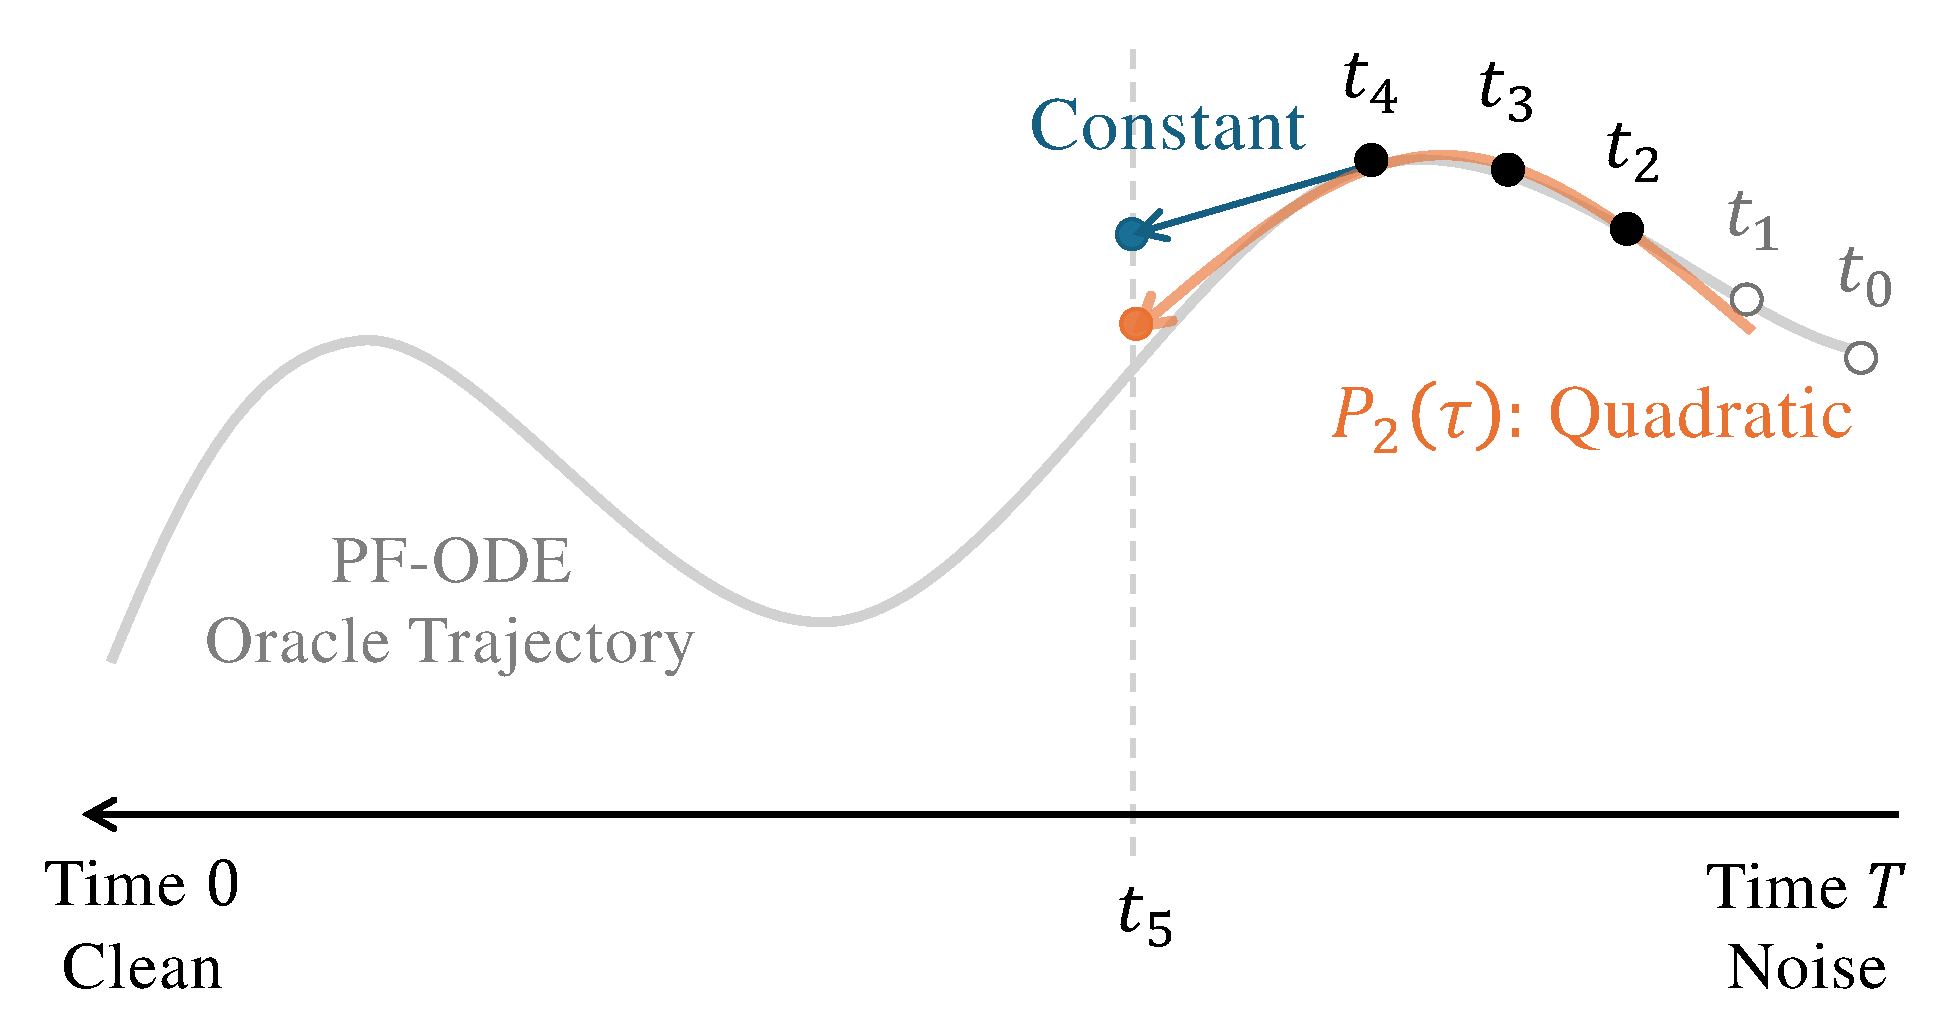
\includegraphics[width=\linewidth]{Images/PartC/DEIS.pdf}
    \caption{\textbfs{Illustration of DEIS as a multistep method.} With three past anchors at
$t_2,t_3,t_4$, DEIS builds a quadratic curve through the model outputs
and analytically integrates it to step from
$t_4$ to $t_5$ (extrapolation). This higher-order
update reduces discretization error compared to first-order methods like
DDIM, which only use the value at $t_4$ (constant approximation of the integral).
\figcredit{Created by the authors.}}
    \label{fig:deis_lagrange}
\end{figure}

A degree-$n$ update needs $n{+}1$ anchors. When they are available (\emph{sufficient history}, $i \ge n{+}1$), we use the full degree-$n$ scheme. In the early steps (\emph{insufficient history}, $i \le n$), we apply the same construction at the highest feasible degree, $i{-}1$, and increase the degree as more anchors accumulate. Below we treat these two scenarios in turn.



\paragraph{Case I: $i = n+1,\dots,M$ (Sufficient History).}
Instead of relying solely on the most recent estimate 
$\bm{\epsilon}_{\bm{\phi}^\times}(\tilde{\rvx}_{t_{i-1}},t_{i-1})$, 
DEIS reuses the last $n{+}1$ model evaluations as anchors,
\[
(\tau_j,\rmY_j) := \bigl(t_{i-1-j}, \bm{\epsilon}_{\bm{\phi}^\times}(\tilde{\rvx}_{t_{i-1-j}},t_{i-1-j})\bigr),
\quad j=0,\dots,n.
\]
as anchors. Viewing $\tau\mapsto\bm{\epsilon}_{\bm{\phi}^\times}(\rvx_\tau,\tau)$ as a smooth function of time along the trajectory, we construct the degree-$n$ polynomial (Lagrange interpolant)
\[
P_n(\tau)
= 
\sum_{j=0}^{n}
\underbrace{\Bigl[\prod_{\substack{k=0\\k\neq j}}^{n}
\frac{\tau - t_{i-1-k}}{\,t_{i-1-j} - t_{i-1-k}\,}\Bigr]}_{=:~\ell_j^{(i)}(\tau)}
\bm{\epsilon}_{\bm{\phi}^\times}\bigl(\tilde{\mathbf x}_{t_{i-1-j}}, t_{i-1-j}\bigr)
\]
which by construction satisfies $P_n(\tau_j)=\rmY_j$ for each anchor:
\[
P_n\bigl(\tau_j\bigr)
= \rmY_j =
\bm{\epsilon}_{\bm{\phi}^\times}\bigl(\tilde{\mathbf x}_{t_{i-1-j}}, t_{i-1-j}\bigr),
\quad
 j=0,\ldots,n.
\]
Each $\ell_j^{(i)}$ satisfies
\[
\ell_j^{(i)}\bigl(t_{i-1-m}\bigr)
=
\begin{cases}
1,&m=j,\\
0,&m\neq j.
\end{cases}
\]

The Lagrange polynomial provides a smooth extrapolation over the new step:
\[
\bm{\epsilon}_{\bm{\phi}^\times}(\rvx_\tau,\tau) \approx
P_n(\tau)=\sum_{j=0}^{n}\ell_j^{(i)}(\tau) 
\bm{\epsilon}_{\bm{\phi}^\times}\bigl(\tilde{\rvx}_{t_{i-1-j}}, t_{i-1-j}\bigr), 
\quad \tau \in [t_{i-1},t_i].
\]
We then substitute $P_r(\tau)$ for $\beps_{\bm{\phi}^\times}(\rvx_\tau,\tau)$ in the
exponential–integrator formula (\Cref{eq:variation_of_constants}):
\begin{align*}
    \int_{t_{i-1}}^{t_i}
\frac{g^2(\tau)}{2 \sigma_\tau} 
\mathcal{E}&(\tau\to t_i) 
\beps_{\bm{\phi}^\times}(\rvx_\tau,\tau)\diff\tau
\\&\approx\sum_{j=0}^{r}
\underbrace{\int_{t_{i-1}}^{t_i}
\frac{g^2(\tau)}{2 \sigma_\tau} 
\mathcal{E}(\tau\to t_i) 
\ell_j^{(i)}(\tau)\diff\tau}_{=:~C_{i,j}} 
\beps_{\bm{\phi}^\times}(\tilde{\rvx}_{t_{i-1-j}},t_{i-1-j}).
\end{align*}
The weights $C_{i,j}$ are given by
\begin{equation*}
C_{i,j} := \frac{1}{2} \int_{t_{i-1}}^{t_i} \frac{g^2(\tau)}{\sigma_\tau} \mathcal{E}(\tau \to t_i) \ell_j^{(i)}(\tau) \diff\tau,
\end{equation*}
depending only on the schedule $(\alpha_\tau,\sigma_\tau)$ and the grid
$\{t_i\}$. Hence, they can be precomputed exactly in closed form once the steps are fixed.

Integrating the linear part exactly with $\mathcal{E}(t_{i-1}\to t_i)$, this leads to the \emph{AB-DEIS-$r$} update rule\footnote{``AB'' refers to the classical
Adams–Bashforth family and exponential time–differencing multistep methods~\citep{hochbruck2010exponential}.},
\[
\tilde{\rvx}_{t_i}
=
\mathcal{E}(t_{i-1}\to t_i) \tilde{\rvx}_{t_{i-1}}
+
\sum_{j=0}^{r} C_{i,j} 
\beps_{\bm{\phi}^\times}(\tilde{\rvx}_{t_{i-1-j}},t_{i-1-j}).
\]
It yields a local truncation
error of order $r{+}1$ under standard smoothness assumptions.




\paragraph{Case II: $i=1,\dots,n$ (Insufficient History).}
For the initial steps, only $i$ past points are available. We therefore set the degree to $i{-}1$ and define
\[
P_{i-1}(\tau)
=
\sum_{j=0}^{i-1}
\ell_j^{(i)}(\tau) 
\bm{\epsilon}_{\bm{\phi}^\times}\bigl(\tilde{\mathbf x}_{t_{i-1-j}},  t_{i-1-j}\bigr),
\]
where $\ell_j^{(i)}$ is the Lagrange basis of degree $i{-}1$ built on the nodes at time
$\{t_{i-1}, t_{i-2},\ldots,t_{0}\}$. This matches all available anchors and
seamlessly transitions into the full‐history formula once $i\ge n{+}1$.

This is a standard ``warm start'' in multistep solvers. When history is short, we fit the richest polynomial the data allow: with one anchor ($i{=}1$), use degree $0$ (constant); with two anchors ($i{=}2$), use degree $1$ (linear); with three anchors ($i{=}3$), use degree $2$ (quadratic); and so on, until we reach the target degree $n$. In effect, we gradually ramp up from a one-step forecast to a true $(n{+}1)$-step forecast as more history becomes available.


\exm{Special Cases of Lagrange Polynomials}{
\noindent \textbfs{When $r=0$ (one anchor):}
\[
P_0(\tau) = \bm{\epsilon}_{\bm{\phi}^\times}(\tilde\rvx_{t_{i-1}}, t_{i-1}).
\]
This uses only the most recent value, so the approximation is flat in $\tau$.
It corresponds to a left-endpoint  of the integrand.

\medskip
\noindent \textbfs{When $r=1$ (two anchors):} the Lagrange polynomial is a linear map passing through the two pre-specified anchors.
\[
P_1(\tau)
= 
\underbrace{\frac{\tau - t_{i-2}}{t_{i-1} - t_{i-2}}}_{\displaystyle \ell_{i-1}(\tau)}
\,\bm{\epsilon}_{\bm{\phi}^\times}(\tilde\rvx_{t_{i-1}}, t_{i-1})
 + 
\underbrace{\frac{\tau - t_{i-1}}{t_{i-2} - t_{i-1}}}_{\displaystyle \ell_{i-2}(\tau)}
\,\bm{\epsilon}_{\bm{\phi}^\times}(\tilde\rvx_{t_{i-2}}, t_{i-2}).
\]
Here $\ell_{i-1}(\tau)$ and $\ell_{i-2}(\tau)$ are the Lagrange basis weights.
They satisfy the interpolation (nodal) conditions
$P_1(t_{i-1})=\bm{\epsilon}_{\bm{\phi}^\times}(\tilde\rvx_{t_{i-1}}, t_{i-1})$ and
$P_1(t_{i-2})=\bm{\epsilon}_{\bm{\phi}^\times}(\tilde\rvx_{t_{i-2}}, t_{i-2})$,
and with
$\ell_{i-1}(\tau)+\ell_{i-2}(\tau)=1$. 
}

\paragraph{Summary of AB-DEIS-$n$ Update.}
Combining the two cases, sufficient history and warm start (insufficient history), yields the
\emph{AB-DEIS-$n$} update\footnote{``AB'' refers to the Adams–Bashforth family of exponential
time–differencing multistep methods~\citep{hochbruck2010exponential}.} where $n$ is the polynomial
degree (using up to $n{+}1$ past evaluations) as follows:
\begin{mdframed}
\begin{align*}
\tilde\rvx_{t_i}
= \mathcal{E}(t_{i-1} \to t_i)\,\tilde\rvx_{t_{i-1}}
+ \sum_{j=0}^{\min\{n,\, i-1\}} C_{i,j}\,\beps_{\bm{\phi}^\times}(\tilde\rvx_{t_{i-1-j}},\,t_{i-1-j}),
\end{align*}
with coefficients
\begin{align*}
C_{i,j}
:= \frac{1}{2} \int_{t_{i-1}}^{t_i}
\frac{g^2(\tau)}{\sigma_\tau}\,\mathcal{E}(\tau \to t_i)\,
\Bigg[\prod_{\substack{k=0\\k\neq j}}^{\min\{n,\, i-1\}}
\frac{\tau - t_{i-1-k}}{\,t_{i-1-j} - t_{i-1-k}\,}\Bigg]\,d\tau.
\end{align*}
\end{mdframed}

When $i\ge n{+}1$ (sufficient history), $\min\{n,\, i-1\}=n$
and the step attains local truncation error $\mathcal O(h^{\,n+1})$ under standard smoothness assumptions.
During warm start ($i\le n$), $\min\{n,\, i-1\}=i-1$ and the per-step order is $\mathcal O(h^{\,\min\{n,\, i-1\}+1})$, ramping up
until full order is reached. 

However, very large $n$ often degrades performance due to interpolation ill-conditioning, noise amplification, and tighter stability constraints; small degrees (e.g., $n \in \{1,2,3\}$) usually provide the best accuracy--stability trade-off.

As we will see in the following subsection, the special case $n{=}0$ reduces to exponential Euler/DDIM.



\subsection{DDIM = AB-DEIS-0}\label{sec:ddim-deis} We observe that when $ n = 0 $ (i.e., constant polynomial), the coefficient simplifies to:
\[
C_{i0} = \frac{1}{2} \int_{t_{i-1}}^{t_{i}} \frac{g^2(\tau)}{\sigma_\tau} \mathcal{E}(\tau \shortrightarrow t_i)   \mathrm{d}\tau.
\]
Substituting into the update formula yields the zeroth-order AB-DEIS scheme:
\begin{align}\label{eq:deis-0}
  \tilde\rvx_{t_{i}} &=  \mathcal{E}(t_{i-1} \shortrightarrow t_{i})\tilde\rvx_{t_{i-1}} + C_{i0} \bm{\epsilon}_{\bm{\phi}^\times}(\tilde\rvx_{t_{i-1}}, t_{i-1})\nonumber\\
  &=e^{\int_{t_{i-1}}^{t_{i}}f(u)\diff u} \tilde\rvx_{t_{i-1}} + \Big( \int_{t_{i-1}}^{t_{i}} \frac{g^2(\tau)}{2\sigma_\tau} e^{\int_{\tau}^{t_{i}}f(u)\diff u}   \mathrm{d}\tau
\Big) \bm{\epsilon}_{\bm{\phi}^\times}(\tilde\rvx_{t_{i-1}}, t_{i-1}).  
\end{align}
This is exactly the exponential–Euler step (constant-in-time $\beps_{\bphi^\times}$ over $[t_{i-1},t_i]$), which
coincides with the deterministic DDIM update. We state this correspondence formally below.
\proppnp{DDIM = AB-DEIS-0}{ddim-deis}{\Cref{eq:deis-0} is identical to the DDIM update in \Cref{eq:ddim-euler}.}


    
\clearpage
\newpage



\section{\texorpdfstring{DPM-Solver}{DPM-Solver}}\label{sec:dpm}

The DPM-Solver family, including DPM-Solver~\citep{lu2022dpm}, DPM-Solver\texttt{++}~\citep{lu2022dpm2}, and DPM-Solver-v3~\citep{zheng2023dpm}, represents a major advance in solvers for the PF-ODE. The goal is simple: achieve similar sample quality with far fewer steps. In practice, these methods reduce the steps required by DDIM from more than $50$ to about $10$-$15$, which makes generation much more efficient. In addition, DPM-Solver\texttt{++} and DPM-Solver-v3 are designed to handle classifier free guidance (CFG) (see \Cref{sec:cfg}) for conditional generation. In this section, we first explain the core DPM-Solver~\citep{lu2022dpm}; its extensions appear in \Cref{sec:dpm++}.

\paragraph{High-Level Idea of DPM-Solver.}
Like DEIS, DPM-Solver starts from the semilinear form of the PF-ODE and works in the $\beps$-prediction parameterization, using the exponential integrator (variation of constants) representation in \Cref{eq:exp-int-factor}:
\begin{align}\label{eq:noise-alpha-sigma}
    \frac{\diff \rvx_t}{\diff t}
= \frac{\alpha_t'}{\alpha_t}\rvx_t
- \sigma_t \left(\frac{\alpha_t'}{\alpha_t}-\frac{\sigma_t'}{\sigma_t}\right)
\beps_{\bphi^\times}(\rvx_t,t).
\end{align}
The key idea is to reparameterize time by the half-log signal-to-noise ratio, so that the nonlinear term in the exponential integrator formula becomes an exponentially weighted integral. This representation admits low-cost Taylor expansions in $\lambda$, which naturally yield higher-order update rules. We will shortly provide an intuitive explanation for why this reparameterization is effective.



\subsection{DPM-Solver's Insight: Time Reparameterization via Log-SNR}\label{subsec:dpm-method}   
On top of the semilinear structure, a key insight from of DPM-solver is that the standard time parameterization $t$ is suboptimal for numerical integration in diffusion models. They instead propose reparameterizing time using the \emph{half-log signal-to-noise ratio} (half-log SNR) 
\begin{align}\label{eq:lambda}
    \lambda_t \coloneqq \frac{1}{2}\log \frac{\alpha_t^2}{\sigma_t^2}  =  \log \frac{\alpha_t}{\sigma_t},
\end{align}
following the log-SNR parameterization of VDM~\citep{kingma2021variational}.
This change-of-variables simplifies the nonlinear integrand, thereby enabling more tractable and accurate higher-order model estimation.







\paragraph{Change-of-Variable to Log-SNR in PF-ODE.} We now reparametrize time using the half–log SNR, $\lambda_t := \log(\alpha_t/\sigma_t)$. 
For common noise schedules, $\lambda_t$ is strictly decreasing in $t$. Under this assumption, it has an inverse function $t_\lambda(\cdot)$ that maps $\lambda$ to $t$, satisfying  
\[
t = t_\lambda(\lambda(t)).
\]  
We then change the subscripts of $\rvx$ and $\bm{\epsilon}_{\bm{\phi}^\times}$ from $t$ to $\lambda$. A hat (  $\hat{\cdot}$  ) indicates that the quantity is expressed in $\lambda$. More precisely, we define:
\begin{align}
\begin{aligned}
    \label{eq:change-of-var-x-epsilon}
 \hat{\rvx}_{\lambda} & := \rvx_{t_\lambda(\lambda)}, \\
 \hat{\bm{\epsilon}}_{\bm{\phi}^\times}(\hat{\rvx}_{\lambda}, \lambda) & \coloneqq \bm{\epsilon}_{\bm{\phi}^\times}(\rvx_{t_\lambda(\lambda)}, t_\lambda(\lambda)).
\end{aligned}
\end{align}

With this change of variables from $t$ to $\lambda_t$, the exact solution $\widetilde\bPsi_{s\to t}$ of  the PF-ODE in \Cref{eq:noise-alpha-sigma} becomes:
\proppp{Exponentially Weighted Exact Solution}{exp-wgt-exact-sol}{Given an initial value $\rvx_s$ at time $s>0$, the exact solution $\widetilde\bPsi_{s\to t}(\rvx_s)$ at time $t\in[0,s]$ of the PF-ODE  can be re-expressed as:
\begin{equation}
\label{eq:analytic_solution}
    \widetilde\bPsi_{s\to t}(\rvx_s) = \frac{\alpha_t}{\alpha_s}\rvx_s - \alpha_t \int_{\lambda_s}^{\lambda_t} e^{-\lambda} \hat{\bm{\epsilon}}_{\bm{\phi}^\times}(\hat\rvx_\lambda,\lambda)\diff \lambda.
\end{equation}}{While one may directly apply the change of variables to \Cref{eq:noise-alpha-sigma} to obtain the result, we provide an alternative derivation below for clarity and completeness.
Using the relation $ g^2(t) = -2\sigma_t^2\frac{\diff \lambda_t}{\diff t} $, \Cref{eq:noise-alpha-sigma} can be rewritten as:
\[
\frac{\diff \rvx_t}{\diff t} = \frac{\diff \log \alpha_t}{\diff t} \rvx_t - \sigma_t \frac{\diff \lambda_t}{\diff t} \bm{\epsilon}_{\bm{\phi}^\times}(\rvx_t, t).
\]
Applying the chain rule:
\[
\frac{\diff \rvx_t}{\diff t} = \frac{\diff \hat\rvx_\lambda}{\diff \lambda} \frac{\diff \lambda_t}{\diff t} \quad \text{and} \quad \frac{\diff \log\alpha_t}{\diff t} = \frac{\diff \log\alpha_\lambda}{\diff \lambda} \frac{\diff \lambda_t}{\diff t},
\]
the ODE in $ t $ is transformed into an ODE in $ \lambda $ as follows:
\begin{align*}
    \frac{\diff \hat\rvx_\lambda}{\diff \lambda} &= \Big(\frac{\diff \lambda_t}{\diff t}\Big)^{-1} \frac{\diff \rvx_t}{\diff t} \\
    &= \Big(\frac{\diff \lambda_t}{\diff t}\Big)^{-1} \Big[ \frac{\diff \log \alpha_t}{\diff t} \rvx_t - \sigma_t \frac{\diff \lambda_t}{\diff t} \bm{\epsilon}_{\bm{\phi}^\times}(\rvx_t, t) \Big] \\
    &= \Big(\frac{\diff \lambda_t}{\diff t}\Big)^{-1} \Big[ \frac{\diff \log\alpha_\lambda}{\diff \lambda} \frac{\diff \lambda_t}{\diff t} \hat\rvx_\lambda - \sigma_\lambda \frac{\diff \lambda_t}{\diff t} \hat{\bm{\epsilon}}_{\bm{\phi}^\times}(\hat\rvx_\lambda, \lambda) \Big] \\
    &= \frac{\diff \log\alpha_\lambda}{\diff \lambda} \hat\rvx_\lambda - \sigma_\lambda \hat{\bm{\epsilon}}_{\bm{\phi}^\times}(\hat\rvx_\lambda, \lambda).
\end{align*}
Thus, the transformed ODE becomes \Cref{eq:diffusion_ode_lambda_eps}. We can then apply the same ``Exponential Integrator (EI)'' technique  to \Cref{eq:diffusion_ode_lambda_eps} to derive \Cref{eq:analytic_solution}.
}

In $\lambda$–time, the model appears inside an exponentially weighted integral,
\[
\int_{\lambda_s}^{\lambda_t} e^{-\lambda} \hat{\bm{\epsilon}}_{\bm{\phi}^\times}(\hat\rvx_\lambda,\lambda) \diff \lambda,
\]
where the $e^{-\lambda}$ factor produces closed-form coefficients and smooths the integrand, exactly what high-order local approximations require.

Equivalently, changing variables from $t$ to $\lambda$ transforms the PF-ODE into the differential form below (see the derivation in the previous proposition):
\begin{mdframed}
\begin{align}\label{eq:diffusion_ode_lambda_eps}
\frac{\diff \hat{\rvx}_\lambda}{\diff \lambda}
= \frac{\alpha_\lambda'}{\alpha_\lambda} \hat{\rvx}_\lambda
- \sigma_\lambda \hat{\bm{\epsilon}}_{\bm{\phi}^\times}(\hat{\rvx}_\lambda, \lambda).
\end{align}
\end{mdframed}


\paragraph{Intuition of Why Reparameterize Time?}
For strictly monotone $\lambda(t)$, the first–order change of variables gives
\[
\Delta t  \approx  \frac{\Delta\lambda}{ |\lambda'(t)| }.
\]
Thus, for fixed $\Delta\lambda$, the induced $\Delta t$ is smaller where $|\lambda'(t)|$ is larger (i.e.\ where $\lambda$ changes rapidly with $t$), and larger where $|\lambda'(t)|$ is smaller. 
This reparameterization does not alter the PF–ODE solution path, only the speed:
\[
\frac{\diff \hat\rvx_\lambda}{\diff \lambda}
= \frac{1}{\lambda'(t)} \frac{\diff \rvx_t}{\diff t}.
\]
Consequently, in regions with large $|\lambda'(t)|$, the $\lambda$–domain derivative is scaled by $1/|\lambda'(t)|$, often making the integrand smoother to approximate on a uniform $\lambda$ grid. 
(The precise location of large $|\lambda'(t)|$ depends on the chosen schedule.) 

Conceptually, we may want to allocate more timesteps when the process gets closer to the complicated (data) distribution. Below are two simple schedules that illustrate this effect:
\begin{itemize}
\item $(\alpha_t,\sigma_t)=(1-t, t)$: This corresponds to the FM scheduler. Then
\[
\lambda(t)=\log\frac{1-t}{t},\quad 
\lambda'(t)=-\frac{1}{t(1-t)},\quad
\Delta t \approx \Delta\lambda   t(1-t).
\]
Hence steps are tiny near both ends ($t\to 0,1$) and largest around mid-time.

\item $(\alpha_t,\sigma_t)=(1, t)$: This is the EDM scheduler~\citep{karras2022elucidating}, introduced in \Cref{sec:edm}. If we take the independent variable directly as the noise level $t=\sigma_t$, then
\[
\lambda(t)=\log\frac{1}{t},\quad 
\lambda'(t)=-\frac{1}{t},\quad
\Delta t \approx \Delta\lambda   t.
\]
Uniform spacing in $\lambda$ is geometric in $t$, or equivalently in the variance (many small steps at small $t$/high SNR, coarser at large $t$).
\end{itemize}




\subsection{Estimating the Integral with Taylor Expansion}\label{subsec:dpm-method-2} 
DEIS approximates the exponentially weighted integral by polynomial
interpolation of the integrand across previous evaluations (a multistep
approach). DPM-Solver starts from the same exact integral formulation
but reparametrizes time by the log-SNR variable~$\lambda$ and derives
high-order updates via a local Taylor expansion in~$\lambda$, using
intermediate staged evaluations within each step (a single-step
approach). Later multistep variants of DPM-Solver are more closely connected to the interpolation-based viewpoint of DEIS, and we return to this comparison in \Cref{sec:summary-solver}. We now present the single-step derivation of DPM-Solver.



From \Cref{eq:analytic_solution}, starting with the previous point $\tilde\rvx_{s}$ at time $s$, the solution $\tilde\rvx_{t} $ at time $t$ is given by
\begin{equation}
\label{eqn:analytic_solution_each_step}
    \tilde\rvx_{t}  = \frac{\alpha_{t}}{\alpha_{s}} \tilde\rvx_{s} - \alpha_{t} \int_{\lambda_{s}}^{\lambda_{t}} e^{-\lambda} \hat{\bm{\epsilon}}_{\bm{\phi}^\times}(\hat\rvx_{\lambda}, \lambda)\diff\lambda.
\end{equation}
Therefore, we are led to approximate integrals of the form:
\begin{align*}
    \int_{\lambda_{s}}^{\lambda_{t}} e^{-\lambda} \hat{\bm{\epsilon}}_{\bm{\phi}^\times}(\hat\rvx_{\lambda}, \lambda)\diff\lambda.
\end{align*}

On the interval $\lambda \in [\lambda_{s}, \lambda_{t_i}]$, we approximate the integrand $\hat{\bm{\epsilon}}_{\bm{\phi}^\times}(\hat\rvx_\lambda, \lambda)$ in \Cref{eqn:analytic_solution_each_step} by a Taylor expansion with respect to $\lambda$. For $n \geq 1$, the $(n{-}1)$-th order Taylor expansion about $\lambda_{s}$ is given by
\begin{equation*}
    \hat{\bm{\epsilon}}_{\bm{\phi}^\times}(\hat\rvx_\lambda, \lambda)
    = \sum_{k=0}^{n-1} \frac{(\lambda - \lambda_{s})^k}{k!} 
    \hat{\bm{\epsilon}}_{\bm{\phi}^\times}^{(k)}(\hat\rvx_{\lambda_{s}}, \lambda_{s})
    + \mathcal{O}((\lambda - \lambda_{s})^n),
\end{equation*}
where the $k$-th total derivative with respect to $\lambda$ is denoted by
\[
\hat{\bm{\epsilon}}_{\bm{\phi}^\times}^{(k)}(\hat\rvx_\lambda, \lambda) 
\coloneqq \frac{\diff^k}{\diff\lambda^k} \hat{\bm{\epsilon}}_{\bm{\phi}^\times}(\hat\rvx_\lambda, \lambda).
\]

Substituting this expansion into the integral in \Cref{eqn:analytic_solution_each_step} yields a closed-form approximation, which defines the $n$-th order solver, referred to as \emph{DPM-Solver-$n$}.

\begin{mdframed}
Starting from the previous step estimation $\tilde\rvx_{s}$,
\begin{equation}
    \label{eq:k-th-expansion}
    \tilde\rvx_{t}  =  \frac{\alpha_{t}}{\alpha_{s}} \tilde\rvx_{s} - \alpha_{t} \sum_{k=0}^{n-1} {\color{cyan}\hat{\bm{\epsilon}}_{\bm{\phi}^\times}^{(k)}(\hat\rvx_{\lambda_{s}},\lambda_{s})} ~{\color{orange}C_k}  + \mathcal{O}(h^{n+1}),
\end{equation}
Here, we denote $h\coloneqq \lambda_{t} - \lambda_{s}$, and define:
\begin{align*}
    {\color{orange}C_k}\coloneqq\int_{\lambda_{s}}^{\lambda_{t}}   e^{-\lambda}  \frac{(\lambda - \lambda_{s})^k}{k!}\diff\lambda.
\end{align*}
${\color{orange}C_k}$ can be precomputed analytically by applying integration by parts $k$ times.
\end{mdframed}
We note that the change of variables $t \mapsto \lambda$ is used
to smooth the integrand and derive coefficients, whereas the solver
returns estimates $\tilde{\rvx}_{t}$ on the $t$-grid.

Below, we illustrate DPM-Solver-1 as an example.


\exm{DPM-Solver-1}{
Consider $n=1$ (first order) for demonstration. Starting from the previous estimated point $\tilde\rvx_{s}$, \Cref{eq:k-th-expansion} simplifies to:
\begin{align}\label{eq:dpm-1}
    \tilde\rvx_{t} &= \frac{\alpha_{t}}{\alpha_{s}} \tilde\rvx_{s} - \alpha_{t} \bm{\epsilon}_{\bm{\phi}^\times}(\tilde\rvx_{s},s) \int_{\lambda_{s}}^{\lambda_{t}} e^{-\lambda}\diff\lambda + \mathcal{O}(h^2) \nonumber \\
    &= \frac{\alpha_{t}}{\alpha_{s}} \tilde\rvx_{s} - \sigma_{t} (e^{h} - 1)\bm{\epsilon}_{\bm{\phi}^\times}(\tilde\rvx_{s},s) + \mathcal{O}(h^2).   
    \end{align}
The above formula is exactly the DDIM update; we prove the equivalence in Proposition~\ref{ddim-dpm}.
}

DPM-Solver-$n$ with $n \geq 2$ requires evaluating the $k^{\text{th}}$-derivative {\color{cyan}$\hat{\bm{\epsilon}}_{\bm{\phi}^\times}^{(k)}(\hat\rvx_\lambda, \lambda)$} for $k \leq n-1$. However, directly computing higher-order derivatives is computationally expensive in practice. \citet{lu2022dpm} also propose efficient approximation methods for these derivatives, which will be detailed in the next subsection.

 
\subsection{Implementation of DPM-Solver-$n$}\label{subsec:dpm-n-method} 

\paragraph{DPM-Solver-$n$ with $n \geq 2$.}
In practice, implementing a higher-order DPM-Solver-$n$ entails the following:
\begin{itemize}
    \item Precomputing the coefficients ${\color{orange}C_k}$;
    \item Approximating the $k^{\text{th}}$ derivative {\color{cyan}$\hat{\bm{\epsilon}}_{\bm{\phi}^\times}^{(k)}(\hat\rvx_\lambda,\lambda)$} for $k \leq n-1$ to circumvent the costly computation of exact higher-order derivatives—a challenge well-studied in the ODE literature~\citep{hochbruck2005explicit,luan2021efficient}. One common strategy is finite difference approximation.
\end{itemize}

We now elaborate on the first two points.


\subparagraph{Precomputing ${\color{orange}C_k}$.} 
Let $s$ and $t$ denote the start and end times, respectively, and define $h := \lambda_t - \lambda_s$. Starting from $\rvx_s$, the analytical expansion of the exact solution to \Cref{eq:variation_of_constants} reads:
\begin{equation}
\label{eq:analytic_expansion}
    \rvx_{t} = \frac{\alpha_{t}}{\alpha_{s}}\rvx_{s} - \sigma_{t} \sum_{k=0}^{n-1} h^{k+1} \varphi_{k+1}(h) \hat{\bm{\epsilon}}_{\bm{\phi}^\times}^{(k)}(\hat\rvx_{\lambda_{s}}, \lambda_{s}) + \mathcal{O}(h^{n+1}),
\end{equation}
where each $\varphi_{k+1}(\cdot)$ admits a closed-form. For $k = 0, 1, 2$, they are:
\begin{align*}
\varphi_1(h) &= \frac{e^h - 1}{h}, &
\varphi_2(h) &= \frac{e^h - h - 1}{h^2}, &
\varphi_3(h) &= \frac{e^h - \frac{h^2}{2} - h - 1}{h^3}.
\end{align*}

\exm{DPM-Solver-2/3 with Exact Derivatives}{For $n = 3$ and discrete time steps with $h := \lambda_{t} - \lambda_{s}$, the expansion becomes:
\begin{equation}\label{eq:example-dpm-solver-3-exact}
\begin{aligned}
    \rvx_{t} = \frac{\alpha_{t}}{\alpha_{s}} \rvx_{s}
    &- \sigma_{t} \left(e^{h} - 1\right) \hat{\bm{\epsilon}}_{\bm{\phi}^\times}(\hat\rvx_{\lambda_{s}}, \lambda_{s}) \\
    &- \sigma_{t} \left(e^{h} - h - 1\right) \hat{\bm{\epsilon}}_{\bm{\phi}^\times}^{(1)}(\hat\rvx_{\lambda_{s}}, \lambda_{s}) \\
    &- \sigma_{t} \left(e^{h} - \frac{h^2}{2} - h - 1\right) \hat{\bm{\epsilon}}_{\bm{\phi}^\times}^{(2)}(\hat\rvx_{\lambda_{s}}, \lambda_{s}) \\
    &+ \mathcal{O}(h^4).
\end{aligned}
\end{equation}}






\subparagraph{Approximating {\color{cyan}$\hat{\bm{\epsilon}}_{\bm{\phi}^\times}^{(k)}(\hat\rvx_\lambda,\lambda)$} for $k \leq n-1$.}
For $n \geq 2$, following the standard approach of single-step ODE solvers~\citep{atkinson2009numerical}, \citet{lu2022dpm} introduce an intermediate timestep $s^{\mathrm{mid}}$ between $s$ and $t$ to approximate higher-order derivatives using function evaluations at $s$ and $s^{\mathrm{mid}}$. We illustrate this with the case of $n = 2$.

Let $\gamma \in (0,1]$ be a hyperparameter specifying an interpolation point within the log-SNR interval $[\lambda_s, \lambda_t]$. 
Given an estimate $\tilde\rvx_s$ at $s$, define
\[
    s^{\mathrm{mid}} = t_\lambda\left(\lambda_s + \gamma h\right), \quad \text{where } h := \lambda_t - \lambda_s,
\]
The intermediate estimate is given by:
\[
    \rvx^{\mathrm{mid}} = \frac{\alpha_{s^{\mathrm{mid}}}}{\alpha_s} \tilde\rvx_s - \sigma_{s^{\mathrm{mid}}} \left(e^{\gamma h} - 1\right) \bm{\epsilon}_{\bm{\phi}^\times}(\tilde\rvx_s, s).
\]
This yields the following second-order approximation:
\begin{align}
\label{eq:dpm-solver-2-app}
\begin{aligned}
    \tilde{\rvx}_{t} = \frac{\alpha_{t}}{\alpha_s} \tilde\rvx_s 
    &- \sigma_{t} \left(e^{h} - 1\right) \bm{\epsilon}_{\bm{\phi}^\times}(\tilde\rvx_s, s) \\
    &- \frac{\sigma_t}{\gamma h} \left(e^{h} - h - 1\right) \left( \bm{\epsilon}_{\bm{\phi}^\times}(\rvx^{\mathrm{mid}}, s^{\mathrm{mid}}) - \bm{\epsilon}_{\bm{\phi}^\times}(\tilde\rvx_s, s) \right)
     +  \mathcal{O}(h^3).
\end{aligned}
\end{align}


With $\gamma=\tfrac12$, the two-stage update in \Cref{alg:dpm-solver-2} is equivalent to
\Cref{eq:dpm-solver-2-app} up to $\mathcal O(h^3)$ (local truncation error).
\begin{algorithm}[H]
    \centering
    \caption{DPM-Solver-2 (with $\gamma=\tfrac12$).}\label{alg:dpm-solver-2}
    \begin{algorithmic}[1]
    \Require initial value $\rvx_T$, time steps $\{t_i\}_{i=0}^M$, model ${\bm{\epsilon}}_{\bm{\phi}^\times}$
        \State $\tilde\rvx_{t_0}\gets\rvx_T$
        \For{$i\gets 1$ to $M$}
        \State $h_i \gets \lambda_{t_i} - \lambda_{t_{i-1}}$
        \State $s_{i}^{\text{mid}} \gets t_{\lambda}\left(\tfrac{\lambda_{t_{i-1}} + \lambda_{t_i}}{2}\right)$
        \State 
    $\rvx_{i}^{\text{mid}} \gets \tfrac{\alpha_{s_i^{\text{mid}}}}{\alpha_{t_{i-1}}} \tilde\rvx_{t_{i-1}} - \sigma_{s_i^{\text{mid}}}\left(e^{\tfrac{h_i}{2}} - 1\right){\bm{\epsilon}}_{\bm{\phi}^\times}(\tilde \rvx_{t_{i-1}},t_{i-1})$ 
    \State  $\tilde\rvx_{t_{i}} \gets \tfrac{\alpha_{t_{i}}}{\alpha_{t_{i-1}}} \tilde\rvx_{t_{i-1}} - \sigma_{t_{i}}\left(e^{h_i} - 1\right){\bm{\epsilon}}_{\bm{\phi}^\times}(\rvx_{i}^{\text{mid}},s_i^{\text{mid}})$
        \EndFor
        \State \Return $\tilde\rvx_{t_M}$
    \end{algorithmic}
\end{algorithm}

\rmkb{
In \Cref{eq:dpm-solver-2-app}, the difference quotient
\[
\hat{\bm{\epsilon}}_{\bm{\phi}^\times}^{(1)}(\hat\rvx_{\lambda_s},\lambda_s)
\approx
\frac{\bm{\epsilon}_{\bm{\phi}^\times}(\rvx^{\mathrm{mid}}, s^{\mathrm{mid}})
      - \bm{\epsilon}_{\bm{\phi}^\times}(\tilde\rvx_s, s)}{\gamma h}
\]
approximates the total $\lambda$–derivative of the model along the trajectory. 
This approximation is accurate up to $\mathcal O(h)$, and in \Cref{eq:dpm-solver-2-app} it is multiplied by the exact $\varphi_2$ coefficient $e^h-h-1=\mathcal O(h^2)$. 
Hence, the resulting contribution is only $\mathcal O(h^3)$, so the overall scheme achieves second-order accuracy for any $\gamma \in (0,1]$.  

Each step requires exactly two model evaluations: one at $(\tilde\rvx_s,s)$ and one at the predicted midpoint $(\rvx^{\mathrm{mid}},s^{\mathrm{mid}})$.  
The interpolation parameter $\gamma$ does not affect the order of accuracy, but it changes the error constant: setting $\gamma=\tfrac12$ symmetrizes the stencil and typically minimizes the constant, which is why the midpoint version is preferred in practice.

}


For higher-order DPM-Solver-$n$ with $n \geq 3$, a similar approach is employed, utilizing intermediate timesteps to approximate higher-order derivatives in a finite difference manner. The detailed methodology is deferred to the original DPM paper.


For readers familiar with numerical ODE solvers, \textsc{DPM-Solver} can be viewed as a 
one-step \emph{exponential integrator} for the semilinear PF-ODE, combined with a change of 
time variable to the (half-)log–SNR. Its second- and third-order variants are exponential 
Runge--Kutta–type schemes that use a few staged model evaluations within each step.


\paragraph{Implementation Detail: Selection of Sampling Timesteps.} To perform sampling, solvers must first predefine a sequence of timesteps $\{t_i\}_{i=0}^M$.  
\citet{lu2022dpm} propose selecting these steps based on \emph{uniform spacing in log–SNR time} $\lambda_t$, where
\[
\lambda_{t_i} = \lambda_T + \frac{i}{M}(\lambda_0 - \lambda_T), \quad i = 0, \dots, M.
\]
This differs from earlier approaches~\citep{ho2020denoising,song2020score} that use uniform spacing directly in the physical time variable~$t$.  
Empirically, DPM-Solver achieves high-quality samples even with very few steps when using uniform $\lambda$ spacing\footnote{Alternatively, adaptive step-size strategies dynamically adjust the timesteps by combining solvers of different orders; see Appendix~C of~\citet{lu2022dpm}.}.

Conceptually, this can be understood geometrically: the accuracy of the local Taylor approximation depends on how smoothly the dynamics evolve in $\lambda$.  
Uniform spacing in $\lambda$ therefore yields approximately uniform local error across the trajectory, resulting in finer (denser) steps in $t$ where the signal dominates (high SNR), and coarser (sparser) steps in the noise-dominated regime.  



Although the derivation operates in $\lambda$–space and the PF–ODE is formulated in a convenient semilinear form in that domain, the pre-trained model and noise schedules $(\alpha_t, \sigma_t)$ are usually defined with respect to the original time variable $t$.  
During sampling, the solver selects nodes that are uniformly spaced in $\lambda$ for numerical stability, but all update equations are expressed in $t$.  
Whenever it needs to evaluate the model or retrieve schedule values, the chosen $\lambda$ node is mapped back to the corresponding time variable, such as the physical time $t = t_\lambda(\lambda)$ or the variance parameter $\sigma_t$, depending on how the model is parameterized (see, for instance, \Cref{alg:dpm-solver-2}).  










\subsection{DDIM $=$ DPM-Solver-1}\label{subsec:ddim=dpm-solver-1}
For a fixed schedule $(\alpha_t,\sigma_t)$, the DPM-Solver-1 step 
coincides with the deterministic DDIM ($\eta=0$) update, 
independent of the time parameterization (physical time $t$ or log--SNR time $\lambda$);
see the formal statement below.
\proppp{DDIM is DPM-Solver-1}{ddim-dpm}{
The update rule of DDIM, given in \Cref{eq:ddim-euler}, is identical to that of DPM-Solver-1, given in \Cref{eq:dpm-1}.
}{
By the definition of $\lambda$, we have
\begin{align}
    \frac{\sigma_s}{\alpha_s} = e^{-\lambda_s} \quad \text{and} \quad \frac{\sigma_t}{\alpha_t} = e^{-\lambda_t}.
\end{align}
Substituting these expressions, along with $h = \lambda_t - \lambda_s$, into \Cref{eq:ddim-euler} recovers the update rule in \Cref{eq:dpm-1}, completing the equivalence.
}
The above proposition may explain why DDIM outperforms traditional Euler methods in $t$-parametrization: it effectively exploits the semilinearity of the diffusion ODE under a more suitable $\lambda$-reparametrization.


\rmkb{When the Score SDE paper appeared, Runge--Kutta (RK45) was commonly used to solve the vanilla PF-ODE in \Cref{eq:prob_ode_sub}, but the semilinearity of its drift remained unexploited. Although DPM-Solver-$k$ ($k \geq 2$) is related to Runge--Kutta methods, it explicitly leverages this semilinearity via a time reparameterization. This explains why DPM-Solver attains higher-order accuracy with far fewer function evaluations, reducing a typical DDIM schedule of several hundred steps to about $10$--$15$ steps while preserving high sample quality.
}





\subsection{Discussion on DPM-Solver-2 and Classic Heun updates}\label{subsec:dpm-heun}

In \Cref{subsec:ddim-different-para}, we saw that different parameterizations of the PF--ODE lead to different interpretations of classical Euler–type updates:
\begin{align*}
\text{$\rvv$-prediction:} 
&\quad \text{Euler} = \text{DDIM}, \\[4pt]
\text{$\beps$-, $\rvx$-, or $\rvs$-prediction:} 
&\quad \text{exp--Euler} = \text{DDIM} \neq \text{plain Euler}.
\end{align*}

In this subsection, we further illustrate the connection by examining the analogous relationship between the classic \emph{Heun's method} and the 2nd–order DPM–Solver across the four parameterizations.


To set the stage, we briefly recall Heun’s method (see also \Cref{app:de-solver}). 
Heun’s method is a 2nd–order solver that refines Euler’s method using a predictor–corrector scheme: 
it first makes an Euler prediction to the end of the step, evaluates the slope there, and then updates using 
the average of the starting and predicted slopes. 
Intuitively, it advances along the curve by following the mean slope over the interval 
(the area of a trapezoid), achieving much higher accuracy than plain Euler.

We work in the log--SNR time $\lambda$, where the PF--ODE can be expressed in a simple ``linear + nonlinear’’ form:
\[
\frac{\diff \hat{\rvx}(\lambda)}{\diff \lambda}
= \underbrace{L(\lambda)\hat{\rvx}(\lambda)}_{\text{linear part}} + \underbrace{\rmN\big(\hat{\rvx}(\lambda),\lambda\big)}_{\text{nonlinear part}},
\]
where the scalar $L(\lambda)$ is determined by the noise schedule and $\rmN(\cdot,\lambda)$ collects the nonlinear part. 
This structure naturally arises from \Cref{eq:clean_pf_ode}: the $\beps$-, $\rvx$-, and $\rvs$-prediction parameterizations yield nonzero $L(\lambda)$, resulting in a semilinear form. 
In contrast, $\rvv$-prediction corresponds to $L(\lambda)\equiv 0$ (so $\rmN=\rvv$), leaving no explicit linear term.


In the remainder of our discussion, we first recall the plain Heun update without considering any semilinear structure, 
and then introduce the exponential Heun update, which is designed for semilinear ODEs and treats the linear part exactly, analogous to the exponential Euler step in \Cref{eq:exp-euler-step,eq:euler-step}.
Finally, we relate both Heun updates to DPM-Solver-2 under the four parameterizations and conclude:
\begin{align*}
\text{$\rvv$-prediction:} 
&\quad \text{Heun} = \text{DPM-Solver-2}, \\[4pt]
\text{$\beps$-, $\rvx$-, or $\rvs$-prediction:} 
&\quad \text{exp-Heun} = \text{DPM-Solver-2} \neq \text{plain Heun}.
\end{align*}

\begin{figure}[th!]
    \centering
    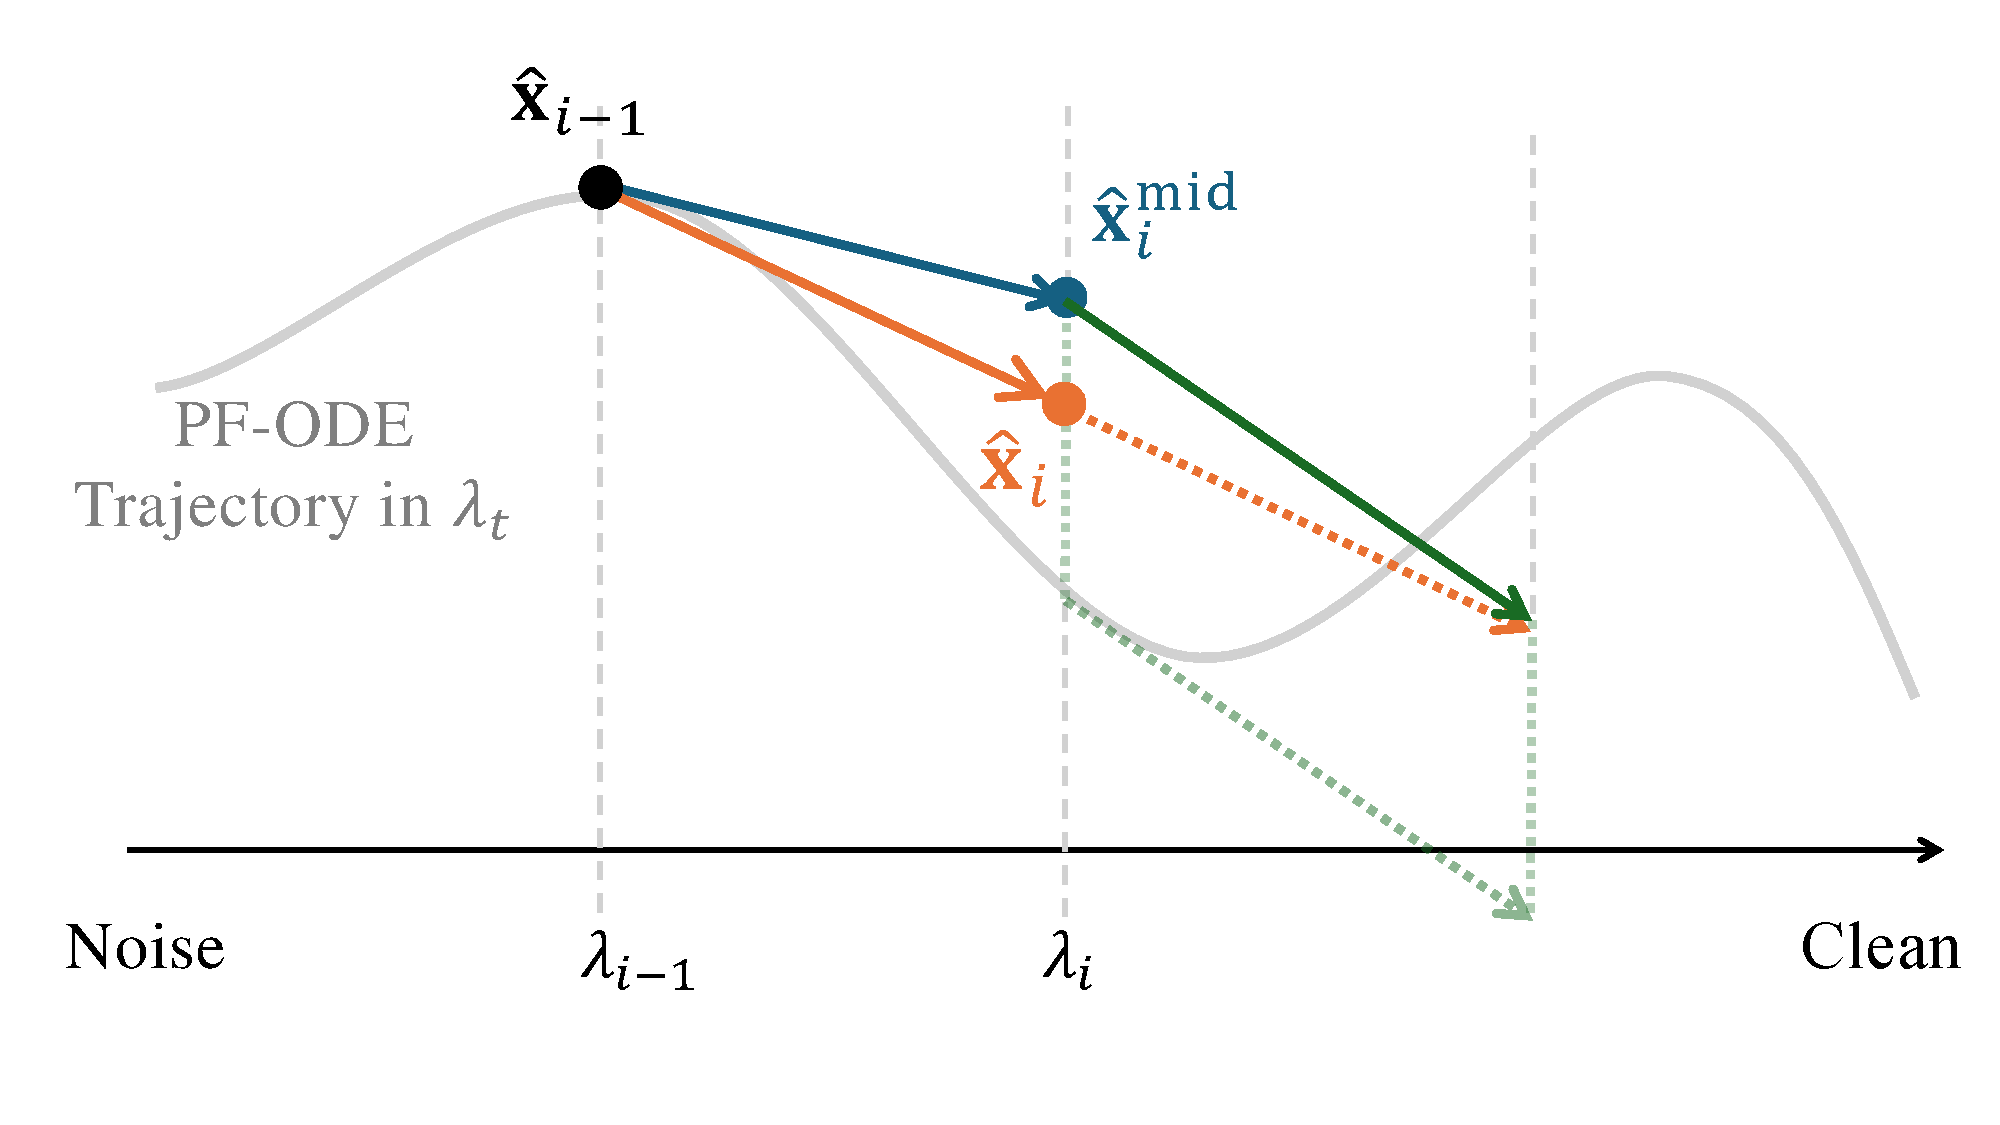
\includegraphics[width=\linewidth]{Images/PartC/Heun.pdf}
\caption{
\textbfs{Plain Heun update in log-SNR time.}
Starting from the previous state $\hat{\mathbf{x}}_{i-1}$ at $\lambda_{i-1}$, 
the \emph{predictor} step (blue arrow) performs an explicit Euler move 
$h \rmF(\hat{\mathbf{x}}_{i-1}, \lambda_{i-1})$ to obtain the intermediate estimate 
$\hat{\mathbf{x}}^{\mathrm{mid}}_i$. 
At this predicted point, the \emph{corrector} step evaluates the new slope 
$h \rmF(\hat{\mathbf{x}}^{\mathrm{mid}}_i, \lambda_i)$ (green arrow) and combines both slopes 
through a parallelogram construction: the dashed orange diagonal represents the vector sum 
$h\big(\rmF(\hat{\rvx}_{i-1},\lambda_{i-1}) + \rmF(\hat{\rvx}^{\mathrm{mid}}_{i},\lambda_{i})\big)$ starting from $\hat\rvx_{i-1}$, 
and the solid orange arrow is its half-diagonal, having the same direction but half the length.
This procedure realizes the plain Heun integration of the PF-ODE trajectory 
in log-SNR time.
\figcredit{Created by the authors.}
}
    \label{fig:plain-heun}
\end{figure}

\paragraph{Plain Heun update.}  
Denote $\lambda_i:=\lambda_{t_i}$, then $\{\lambda_i\}_{i=0}^M$ is an increasing grid in the log-SNR domain, and set $h := \lambda_i - \lambda_{i-1} > 0$. 
Let $\hat{\rvx}_{i-1}$ denote the previous iterate in log-SNR time. 
 Applied directly to the full drift 
\[
\rmF(\hat{\rvx}, \lambda) := L(\lambda) \hat{\rvx} + \rmN(\hat{\rvx}, \lambda),
\]
the plain Heun update in log-SNR-time is given by
\begin{align}\label{eq:heun-logsnr}
\begin{aligned}
    \text{Predict:}\quad 
&\hat{\rvx}^{\mathrm{mid}}_i 
= \hat{\rvx}_{i-1} + h \rmF(\hat{\rvx}_{i-1},\lambda_{i-1}),\\
\text{Correct:}\quad 
&\hat{\rvx}_{i} 
= \hat{\rvx}_{i-1} + \tfrac{h}{2}\Big(\rmF(\hat{\rvx}_{i-1},\lambda_{i-1}) + \rmF(\hat{\rvx}^{\mathrm{mid}}_{i},\lambda_{i})\Big).
\end{aligned}
\end{align}

\paragraph{Exponential Heun update (for Semilinear PF-ODE).} With the \emph{exponential integrator} technique, the idea is to treat the linear and nonlinear parts of the ODE differently.  
The linear term $L(\lambda)\hat{\rvx}$ is integrated exactly over the step, 
while the nonlinear term $\rmN(\hat{\rvx},\lambda)$ is only approximated by averaging its effect across the step.  

To express this neatly, we introduce the quantity
\[
\mathcal{E} := \int_{\lambda_{i-1}}^{\lambda_{i}} L(\tau) \diff\tau,
\]
which represents the total contribution of the linear coefficient $L(\lambda)$ over the interval $[\lambda_{i-1}, \lambda_i]$.
Using $\mathcal{E}$, we define two helper coefficients $c_1(\mathcal{E})$ and $c_2(\mathcal{E})$ that handle both cases:
when $\mathcal{E}$ is nonzero and when it vanishes:
\[
c_1(\mathcal{E}) =
\begin{cases}
\tfrac{e^{\mathcal{E}} - 1}{\mathcal{E}}, & \text{if } \mathcal{E}\neq 0,\\[6pt]
1, & \text{if } \mathcal{E}=0,
\end{cases}
\qquad
c_2(\mathcal{E}) =
\begin{cases}
\tfrac{e^{\mathcal{E}} - 1 - \mathcal{E}}{\mathcal{E}^2}, & \text{if } \mathcal{E}\neq 0,\\[6pt]
\tfrac{1}{2}, & \text{if } \mathcal{E}=0.
\end{cases}
\]
The second case simply ensures continuity when the linear term disappears ($L(\lambda)=0$), so that the formulas remain valid and reduce smoothly to the standard Heun update as in \Cref{eq:heun-logsnr}.

With these coefficients, one update step of the exponential–Heun scheme can be written as:
\begin{align}\label{eq:exp-heun-logsnr}
\begin{aligned}
    \text{Predict:}\quad 
&\hat{\rvx}^{\mathrm{mid}}_{i} 
= e^{\mathcal{E}}\hat{\rvx}_{i-1} + h c_1(\mathcal{E}) \rmN(\hat{\rvx}_{i-1},\lambda_{i-1}),\\
\text{Correct:}\quad 
&\hat{\rvx}_{i} 
= e^{\mathcal{E}}\hat{\rvx}_{i-1}
\begin{aligned}[t]
    &+ h c_1(\mathcal{E}) \rmN(\hat{\rvx}_{i-1},\lambda_{i-1})
\\&+ h c_2(\mathcal{E})\Big(\rmN(\hat{\rvx}^{\mathrm{mid}}_{i},\lambda_{i})-\rmN(\hat{\rvx}_{i-1},\lambda_{i-1})\Big).
\end{aligned}
\end{aligned}
\end{align}

When $L(\lambda)\equiv 0$, the coefficients simplify to $c_1=1$ and $c_2=\tfrac{1}{2}$, and the method reduces to the plain Heun solver in \Cref{eq:heun-logsnr}.  

When $L(\lambda)\neq 0$, the exponential–integrator form of the update integrates the linear term
exactly, while the plain Heun method only provides an approximation. 
To see this, expand the exponential term for a small stepsize 
$h = \lambda_i - \lambda_{i-1} > 0$. 
Since 
\[
\mathcal{E} = \int_{\lambda_{i-1}}^{\lambda_i} L(\tau)\diff\tau 
= h L(\lambda_{i-1}) + \mathcal O(h^2),
\]
we can treat $\mathcal{E}$ as a small quantity of order $\mathcal O(h)$.  The Taylor expansions give:
\[
e^{\mathcal{E}} = 1 + \mathcal{E} + \tfrac{\mathcal{E}^2}{2} + \mathcal O(\mathcal{E}^3),\,\,
c_1(\mathcal{E}) = 1 + \tfrac{\mathcal{E}}{2} + \tfrac{\mathcal{E}^2}{6} + \mathcal O(\mathcal{E}^3),\,\,
c_2(\mathcal{E}) = \tfrac{1}{2} + \tfrac{\mathcal{E}}{6} + \tfrac{\mathcal{E}^2}{24} + \mathcal O(\mathcal{E}^3).
\]

Substituting these approximations into \Cref{eq:exp-heun-logsnr} and keeping terms 
up to $\mathcal{E}^2$ (that is, up to order $h^2$ since $\mathcal{E}=\mathcal{O}(h)$),
the update simplifies exactly to the plain Heun form (\Cref{eq:heun-logsnr}).  
The remaining difference between the two schemes appears only in higher-order terms 
of size $\mathcal{O}(\mathcal{E}^3)=\mathcal{O}(h^3)$.  
Intuitively, when the step size $h$ is small, $\mathcal{E}$ is also small, so the exponential factors 
reduce to 
\[
e^{\mathcal{E}} \approx 1+\mathcal{E},\quad 
c_1(\mathcal{E}) \approx 1,\quad c_2(\mathcal{E}) \approx \tfrac{1}{2}.
\]
The ``linear–handled'' exponential–Heun update thus collapses to the plain Heun step.

\paragraph{Connection of Heun’s Updates to DPM–Solver-2 Under the Four Predictions.}
We highlight that, in the $\beps$-prediction form of the PF-ODE (see \Cref{eq:diffusion_ode_lambda_eps}), 
the dynamics in log–SNR time $\lambda$ naturally take the required semilinear form:
\[
\frac{\diff \hat{\rvx}_\lambda}{\diff \lambda}
= \underbrace{\frac{\alpha_\lambda'}{\alpha_\lambda}}_{=:L(\lambda)} \hat{\rvx}_\lambda
+
\underbrace{\big(- \sigma_\lambda \hat{\bm{\epsilon}}_{\bm{\phi}^\times}(\hat{\rvx}_\lambda,\lambda)\big)}_{=:\rmN(\hat{\rvx}_\lambda,\lambda)}.
\]
Consequently, for $\beps$-prediction in log–SNR time $\lambda$, the exponential–Heun update 
in \Cref{eq:exp-heun-logsnr} is \emph{exactly equivalent} to DPM-Solver-2 
(with midpoint parameter $\gamma=\tfrac{1}{2}$; see \Cref{alg:dpm-solver-2}).

Similarly, under the $\rvx$- and $\rvs$-prediction parameterizations in log–SNR time, 
their PF-ODEs also take the same semilinear structure. 
Hence, the DPM-Solver-2 under the $\beps$-, $\rvx$-, or $\rvs$-prediction 
is \emph{identical} to the exponential–Heun update in \Cref{eq:exp-heun-logsnr}. In contrast, the $\rvv$-prediction form naturally removes the linear term, 
so its PF-ODE does not require an exponential integrator; 
the plain Heun method in log–SNR time already provides the correct 2nd–order update.

Similar to the case of Euler versus exponential Euler in DDIM, we therefore conclude the following: \msg{Observation}{Heun and DPM-Solver-2 Updates}{
Given the PF-ODEs in log-SNR time $\lambda$,
\begin{align*}
\text{$\rvv$-prediction:} 
&\quad \text{Heun} = \text{DPM-Solver-2}, \\[4pt]
\text{$\beps$-, $\rvx$-, or $\rvs$-prediction:} 
&\quad \text{exp-Heun} = \text{DPM-Solver-2} \neq \text{plain Heun},
\end{align*}
where, in the $\beps$-, $\rvx$-, or $\rvs$-prediction cases, the plain Heun step 
is not equivalent to DPM-Solver-2, since the linear term is only approximated 
instead of being integrated exactly.
}




\clearpage
\newpage

\section{\texorpdfstring{DPM-Solver\texttt{++}}{DPM-Solver\texttt{++}}}\label{sec:dpm++}


\subsection{From DPM-Solver to DPM-Solver\texttt{++} for Guidance}
High-order solvers enable faster sampling without guidance. However, diffusion models are prized for their controllable and flexible generation, typically achieved via guidance (see \Cref{ch:guidance} for details).

DPM-Solver\texttt{++}~\citep{lu2022dpm2} identifies a key limitation of prior high-order solvers: they suffer from stability issues and may become slower than DDIM under large guidance scales (stronger condition). The authors attribute this instability to the amplification of both the output and its derivatives by large guidance scales. Since high-order solvers depend on higher-order derivatives, they are especially sensitive to this effect, resulting in diminished efficiency and stability.


\subsection{DPM-Solver\texttt{++}'s Methodology}
To address the aforementioned issues, DPM-Solver\texttt{++} proposes:
\begin{enumerate}
    \item adopting $\rvx$-prediction parameterization instead of $\beps$-prediction;
    \item applying thresholding methods (e.g., dynamic thresholding~\citep{saharia2022photorealistic}) to keep the predicted data within the training data bounds (mitigating the train-test mismatch at large guidance scales).
\end{enumerate}

We elaborate on the first point. Recall from \Cref{eq:predictions-equivalence} that the data and noise parameterizations are linearly related:  
\[
\bm{\epsilon}_{\bm{\phi}^\times}(\rvx_t, t) = \frac{\rvx_t - \alpha_t \rvx_{\bm{\phi}^\times}(\rvx_t, t)}{\sigma_t}.
\]  
Using this relation, DPM-Solver\texttt{++} rewrites the exact solution $\widetilde\bPsi_{s\to t}(\rvx_s)$ of the empirical PF-ODE (originally expressed in the noise parameterization in \Cref{eq:analytic_solution}), starting from any $\rvx_s$:
\[
    \widetilde\bPsi_{s\to t}(\rvx_s)
    = \frac{\alpha_t}{\alpha_s}\rvx_s
      - \alpha_t \int_{\lambda_s}^{\lambda_t}
        e^{-\lambda}  \hat{\bm{\epsilon}}_{\bm{\phi}^\times}(\hat\rvx_\lambda, \lambda)  \mathrm{d}\lambda,
\]
into the data parameterization as
\[
    \widetilde\bPsi_{s\to t}(\rvx_s)
    = \frac{\sigma_t}{\sigma_s}\rvx_s
      + \sigma_t \int_{\lambda_s}^{\lambda_t}
        e^{\lambda}  \hat{\rvx}_{\bm{\phi}^\times}(\hat\rvx_\lambda, \lambda)  \mathrm{d}\lambda,
\]
where we follow the notations in \Cref{eq:change-of-var-x-epsilon} and further denote:
\begin{align*}
\begin{aligned}
 \hat{\rvx}_{\lambda} & := \rvx_{t_\lambda(\lambda)}, \\
 \hat{\rvx}_{\bm{\phi}^\times}(\hat{\rvx}_{\lambda}, \lambda) & \coloneqq \rvx_{\bm{\phi}^\times}(\rvx_{t_\lambda(\lambda)}, t_\lambda(\lambda)).
\end{aligned}
\end{align*}

Based on the $\rvx$-prediction, DPM-Solver\texttt{++} provides two solver variants:
\begin{itemize}
    \item \textbfs{Higher-Order Single-Step Solver:} Introduced in \Cref{subsec:dpm-solver++-single}. This approach is analogous to that in DPM-Solver, which leverages higher-order Taylor expansions to approximate the integration, but here formulated with the $\rvx$-prediction. The update uses only one previous point to estimate the next step.  
    \item \textbfs{Multistep (Two-Step) Solver:} Introduced in \Cref{subsec:dpm-solver++-multi}. The design philosophy is similar to DEIS (also multistep); however, DPM-Solver\texttt{++} specifically reuses two previous points (whereas DEIS allows a general order) to estimate the next step. Each update requires only a single new diffusion model evaluation. 
\end{itemize}


\subsection{DPM-Solver\texttt{++} Single-Step by Taylor Expansion}\label{subsec:dpm-solver++-single}
Following a similar approach to \Cref{subsec:dpm-n-method}, DPM-Solver\texttt{++} derives higher-order solvers in the $\rvx$-parameterization. For $n \ge 0$, denote the $n$-th total derivative of $\hat{\rvx}_{\bphi^\times}$ with respect to $\lambda$, evaluated at $\lambda_{i-1}$, by
\[
\hat{\rvx}_{\bphi^\times}^{(n)}(\hat{\rvx}_{\lambda_{i-1}}, \lambda_{i-1})
:= \left.\frac{\diff^{n}}{\diff \lambda^{n}}\,
\hat{\rvx}_{\bphi^\times}(\hat{\rvx}_\lambda, \lambda)\right|_{\lambda=\lambda_{i-1}}.
\]
Given the previous estimate $\tilde\rvx_{t_{i-1}}$ at time $t_{i-1}$, using the $(n-1)$-th Taylor expansion at $\lambda_{t_{i-1}}$ to approximate $\hat{\rvx}_{\bm{\phi}^\times}(\hat\rvx_\lambda, \lambda)$ for $\lambda \in [\lambda_{t_{i-1}},\lambda_{t_i}]$ (with $s=t_{i-1}$ and $t=t_i$) yields the following approximation of $\widetilde\bPsi_{s\to t}(\rvx_s)$:
\begin{align*} 
\tilde\rvx_{t_i} = \frac{\sigma_{t_i}}{\sigma_{t_{i-1}}}\,\tilde\rvx_{t_{i-1}} + \sigma_{t_i} \sum_{k=0}^{n-1} \underbrace{\hat{\rvx}_{\bphi^\times}^{(k)}(\hat{\rvx}_{\lambda_{i-1}}, \lambda_{i-1})}_{\substack{\text{estimated via} \\ \text{finite difference}}} &\underbrace{\int_{\lambda_{t_{i-1}}}^{\lambda_{t_{i}}}e^\lambda \frac{(\lambda - \lambda_{t_{i-1}})^k}{k!} \diff \lambda}_{\mathrm{analytically\,\,computable}} 
\\ &\quad\quad+ \mathcal O(h_i^{n+1}). 
\end{align*}
where $h_i:=\lambda_{t_i}-\lambda_{t_{i-1}}>0$. As in \Cref{eq:analytic_expansion}, the integral admits the closed form
\[
\int_{\lambda_{t_{i-1}}}^{\lambda_{t_i}}
e^\lambda \frac{(\lambda-\lambda_{t_{i-1}})^k}{k!} \diff\lambda
=
e^{\lambda_{t_{i-1}}} h_i^{\,k+1} \varphi_{k+1}(h_i),
\quad
\varphi_{m}(h):=\frac{e^{h}-\sum_{j=0}^{m-1} \frac{h^{j}}{j!}}{h^{m}}.
\]

This yields the DPM-Solver\texttt{++}'s single-step update (one previous point to estimate the next). When $n=1$, it reduces to the DDIM update. When $n=2$ and $\hat{\rvx}_{\bphi^\times}^{(1)}(\hat{\rvx}_{\lambda_{i-1}}, \lambda_{i-1})$ is approximated via a finite difference, it gives \emph{DPM-Solver\texttt{++}(2S)}, an update analogous to DPM-Solver-2 in \Cref{alg:dpm-solver-2} but using the $\rvx$-prediction. DPM-Solver\texttt{++}(2S)’s algorithm is shown in \Cref{alg:dpmpp-2s-mid}.
\begin{algorithm}[H]
    \centering
    \caption{DPM-Solver\texttt{++}(2S): a midpoint special case.}
    \label{alg:dpmpp-2s-mid}
    \begin{algorithmic}[1]
    \Require initial value $\rvx_T$, time steps $\{t_i\}_{i=0}^M$, data-prediction model $\hat{\rvx}_{\bphi^\times}$
    \State $\tilde\rvx_{t_0}\gets\rvx_T$;\quad $\lambda_{t_i}\gets \log(\alpha_{t_i}/\sigma_{t_i})$ \Comment{log-SNR at the grid}
    \State $\hat\rvx_0 \gets \hat{\rvx}_{\bphi^\times}(\tilde\rvx_{t_0},t_0)$ \Comment{cache at start}
    \For{$i\gets 1$ \textbf{to} $M$}
        \State $h_i \gets \lambda_{t_i}-\lambda_{t_{i-1}}$;\quad $s_i^{\text{mid}} \gets t_{\lambda} \Big(\tfrac{\lambda_{t_{i-1}}+\lambda_{t_i}}{2}\Big)$
        \State $\rvu_i \gets \tfrac{\sigma_{s_i^{\text{mid}}}}{\sigma_{t_{i-1}}}\,\tilde\rvx_{t_{i-1}}
                 + \alpha_{s_i^{\text{mid}}}\big(1-e^{-h_i/2}\big)\,\hat\rvx_{i-1}$ \Comment{forecast to midpoint}
        \State $\rmD_i^{\mathrm{mid}} \gets \hat{\rvx}_{\bphi^\times}(\rvu_i,s_i^{\text{mid}})$ \Comment{one new model call at the midpoint}
        \State $\tilde\rvx_{t_i} \gets \tfrac{\sigma_{t_i}}{\sigma_{t_{i-1}}}\,\tilde\rvx_{t_{i-1}}
               - \alpha_{t_i}\big(e^{-h_i}-1\big)\rmD_i^{\mathrm{mid}}$ 
        \State $\hat\rvx_i \gets \hat{\rvx}_{\bphi^\times}(\tilde\rvx_{t_i},t_i)$ \Comment{cache for next step}
    \EndFor
    \State \Return $\tilde\rvx_{t_M}$
    \end{algorithmic}
\end{algorithm}





\subsection{DPM-Solver\texttt{++} Multistep by Recycling History}\label{subsec:dpm-solver++-multi}
High–order single–step solvers rely (explicitly or implicitly) on higher derivatives of the model output; under strong CFG these derivatives can be strongly amplified and destabilize the update. 
DPM-Solver\texttt{++} mitigates this with a \emph{multistep} (Adams–type) strategy in log-SNR time~$\lambda$: it reuses a short history of past data-prediction evaluations along the trajectory to approximate the needed derivatives via finite differences. 
This reuse requires only one new model call per step. 
As with DEIS, we separate the presentation into: Case 1. the warm start with no history (first step); Case 2. subsequent steps with two history anchors.


\paragraph{Case I. DPM-Solver\texttt{++} with One History Anchor ($i= 1$).}
For the first step ($i=1$; no history), use the first–order DPM-style update (which matches the deterministic DDIM step in data prediction). Let $h_1=\lambda_1-\lambda_0$.
\[
\tilde{\rvx}_{t_1}
=
\frac{\sigma_{t_1}}{\sigma_{t_0}} \tilde{\rvx}_{t_0}
 + 
\sigma_{t_1}\,e^{\lambda_{0}}\,(e^{h_1}-1) 
\hat{\rvx}_{\bm{\phi}^\times}(\tilde{\rvx}_{t_0},t_0)
\]

\paragraph{Case II. DPM-Solver\texttt{++} with Two History Anchors ($i\geq 2$).} 



After the warm start, the two–step multistep update reuses the estimations at time $t_{i-2}$ with $\tilde\rvx_{t_{i-2}}$ and at time $t_{i-1}$ with $\tilde\rvx_{t_{i-1}}$. 
At each step $i\ge2$, these provide the two most recent anchors, equivalently in $\lambda$–time:
\[
(\lambda_{i-1},\,\hat\rvx_{\bm{\phi}^\times}(\tilde\rvx_{t_{i-1}},t_{i-1}))
\quad\text{and}\quad
(\lambda_{i-2},\,\hat\rvx_{\bm{\phi}^\times}(\tilde\rvx_{t_{i-2}},t_{i-2})),
\]
to compute the update $\tilde{\rvx}_{t_i}$ using only these cached anchors (no fresh model call is needed to form the update). 
After obtaining $\tilde{\rvx}_{t_i}$, we evaluate the model once at $(\tilde{\rvx}_{t_i},t_i)$ and cache
$\hat\rvx_{\bphi^\times}(\tilde{\rvx}_{t_i},t_i)$.
This evaluation is performed during step $i$ and is used as an anchor in the subsequent step $i{+}1$. Namely, we aim for a  one–call–per–step update that remains stable under large guidance by discretizing the exact $\rvx$–prediction form
\begin{align*}
    \widetilde\bPsi_{s\to t}(\rvx_s)
= \frac{\sigma_t}{\sigma_s} \rvx_s
 + 
\sigma_t \int_{\lambda_s}^{\lambda_t}  e^{\lambda} 
\hat\rvx_{\bm{\phi}^\times}(\hat\rvx_\lambda,\lambda) \diff\lambda.
\end{align*}
 
Over a single step $[\lambda_{i-1},\lambda_i]$, we treat the linear ODE part exactly and approximate the residual integral by approximating the integrand as a function linear in $\lambda$ (since there are two anchor points). 
Concretely, we approximate
\[
\lambda  \mapsto  \hat\rvx_{\bm{\phi}^\times}(\hat\rvx_{\lambda},\lambda)
\]
on $[\lambda_{i-1},\lambda_i]$ by the affine model
\[
\hat\rvx_{\bm{\phi}^\times}(\hat\rvx_{\lambda},\lambda) 
 \approx  \rmL(\lambda):=\rva_0+\rva_1(\lambda-\lambda_{i-1}), 
\quad \lambda \in [\lambda_{i-1},\lambda_i],
\]
where $\lambda_i=\lambda_{t_i}$, $h_i=\lambda_i-\lambda_{i-1}>0$, and the coefficients $\rva_0$ and $\rva_1$ are uniquely specified by the 
straight line passing through the two most recent anchors:
\[
\rva_0=\hat\rvx_{\bm{\phi}^\times}(\tilde\rvx_{t_{i-1}},t_{i-1}), 
\quad
\rva_1=\frac{\hat\rvx_{\bm{\phi}^\times}(\tilde\rvx_{t_{i-1}},t_{i-1})-\hat\rvx_{\bm{\phi}^\times}(\tilde\rvx_{t_{i-2}},t_{i-2})}{h_{i-1}}.
\]


Substituting $\rmL(\lambda)$ into the integral thus yields\footnote{The second identity follows from a straightforward algebra. The two needed exponential moments are
\[
\int_{\lambda_{i-1}}^{\lambda_i}  e^\lambda \diff\lambda=e^{\lambda_{i-1}}(e^{h_i}-1),
\quad
\int_{\lambda_{i-1}}^{\lambda_i}  e^\lambda(\lambda-\lambda_{i-1}) \diff\lambda
=e^{\lambda_{i-1}} \big(h_i e^{h_i}-e^{h_i}+1\big).
\]
Multiplying by the prefactor $\sigma_{t_i}$ from the exact form and using $\alpha_t=\sigma_t e^{\lambda_t}$ (so $\sigma_{t_i}e^{\lambda_{i-1}}=\alpha_{t_i}e^{-h_i}$) gives the convenient coefficients
\[
\sigma_{t_i} \int_{\lambda_{i-1}}^{\lambda_i} e^\lambda \diff\lambda=\alpha_{t_i}(1-e^{-h_i}),
\quad
\sigma_{t_i} \int_{\lambda_{i-1}}^{\lambda_i} e^\lambda(\lambda-\lambda_{i-1}) \diff\lambda=\alpha_{t_i}(h_i-1+e^{-h_i}).
\]}
\begin{align*}
\sigma_{t_i}\int_{\lambda_{i-1}}^{\lambda_i} e^\lambda \hat\rvx_{\bm{\phi}^\times}(\tilde\rvx_{\lambda},\lambda) \diff\lambda
&\approx \sigma_{t_i}\int_{\lambda_{i-1}}^{\lambda_i} e^\lambda \rmL(\lambda) \diff\lambda \\
&=\left(\sigma_{t_i}\int_{\lambda_{i-1}}^{\lambda_i} e^\lambda \diff\lambda \right)\rva_0+\left(\sigma_{t_i}\int_{\lambda_{i-1}}^{\lambda_i} e^\lambda(\lambda-\lambda_{i-1}) \diff\lambda \right) \rva_1
\\&=\left(\alpha_{t_i}(1-e^{-h_i})\right)\rva_0+\left(\alpha_{t_i}(h_i-1+e^{-h_i}) \right) \rva_1
\\&=\alpha_{t_i}(1-e^{-h_i})\Big(\rva_0+\beta(h_i)  \rva_1\Big),
\end{align*}
where $\beta(h):=\frac{h-1+e^{-h}}{ 1-e^{-h} }$. Until this point, we have already reached a valid estimate for $\tilde\rvx_{t_i}$ as:
\begin{equation*}
\tilde\rvx_{t_i}
=
\frac{\sigma_{t_i}}{\sigma_{t_{i-1}}} \tilde\rvx_{t_{i-1}}
 + 
\alpha_{t_i} \big(1-e^{-h_i}\big) \rmD_i,\quad\text{with } \rmD_i=\rva_0+\beta(h_i)  \rva_1.
\end{equation*}


In practice, we can obtain a simplified update rule with the same local truncation error (provided the step ratios are bounded) as the above one:

\begin{mdframed}
\begin{align*}
\begin{aligned}
    \tilde\rvx_{t_i}=
\frac{\sigma_{t_i}}{\sigma_{t_{i-1}}} \tilde\rvx_{t_{i-1}}
+ 
\alpha_{t_i} \big(1-e^{-h_i}\big) \rmD_i^{\mathrm{sim}}(\tilde\rvx_{t_{i-1}}, \tilde\rvx_{t_{i-2}}).
\end{aligned}
\end{align*}
Here, we define the step ratio $r_i=h_i/h_{i-1}$, and
\begin{align*}
    \rmD_i^{\mathrm{sim}}(\tilde\rvx_{t_{i-1}}, \tilde\rvx_{t_{i-2}})
:=\Big(1+\tfrac12 r_i\Big) \hat\rvx_{\bm{\phi}^\times}(\tilde\rvx_{t_{i-1}},t_{i-1})
-\tfrac12 r_i \hat\rvx_{\bm{\phi}^\times}(\tilde\rvx_{t_{i-2}},t_{i-2}).
\end{align*}
\end{mdframed}
with local error $\mathcal{O}(h_i^3)$ under standard smoothness assumptions. 

To see why, for notational simplicity, we write
\[
\rva_0=\hat\rvx_{\bm{\phi}^\times}(\tilde\rvx_{t_{i-1}},t_{i-1})=:\hat\rvx_{i-1},\quad
\rva_1=\frac{\hat\rvx_{i-1}-\hat\rvx_{i-2}}{h_{i-1}}.
\]
Then
\begin{align*}
\rmD_i
&:= \rva_0+\beta(h_i)\,\rva_1 
\\
&= \hat\rvx_{i-1} + \frac{\beta(h_i)}{h_{i-1}}\big(\hat\rvx_{i-1}-\hat\rvx_{i-2}\big)
\\
&= \Big(1+\tfrac{r_i}{2}\Big)\hat\rvx_{i-1} - \tfrac{r_i}{2}\hat\rvx_{i-2}
   + \Big(\tfrac{\beta(h_i)}{h_{i-1}}-\tfrac{r_i}{2}\Big)\big(\hat\rvx_{i-1}-\hat\rvx_{i-2}\big)
\\
&= \left[\Big(1+\tfrac12 r_i\Big)\hat\rvx_{i-1}-\tfrac12 r_i\,\hat\rvx_{i-2}\right]
   + \mathcal O(h_i^2)
   \\&=\rmD_i^{\mathrm{sim}}
   + \mathcal O(h_i^2)
\end{align*}
Here, we use that for small steps, a Taylor expansion of $\beta(h)$ at $h=0$ gives
\[
\beta(h)=\frac{h}{2}+\mathcal{O}(h^{2})
\,\implies\,
\frac{\beta(h_i)}{h_{i-1}}
=\frac{h_i}{2h_{i-1}}+\mathcal{O}(h_i^{2}/h_{i-1})
=\frac{r_i}{2}+\mathcal{O}(h_i^{2}/h_{i-1}),
\]
and that $\hat\rvx_{i-1}- \hat\rvx_{i-2} = \mathcal{O}(h_{i-1})$ under some smoothness assumption.

\rmkb{
If the log-SNR steps are uniform (every step has the same size $h$, so $h_i\equiv h$ and $r_i=h_i/h_{i-1}=1$), then the two-anchor blend
\[
\rmD_i^{\mathrm{sim}}=\Bigl(1+\tfrac12 r_i\Bigr)\hat\rvx_{i-1}-\tfrac12 r_i\,\hat\rvx_{i-2}
\]
reduces to the classic constants
\[
\rmD_i^{\mathrm{sim}}=\Bigl(1+\tfrac12\cdot 1\Bigr)\hat\rvx_{i-1}-\tfrac12\cdot 1\,\hat\rvx_{i-2}
=\tfrac{3}{2}\,\hat\rvx_{i-1}-\tfrac{1}{2}\,\hat\rvx_{i-2}.
\]
Those $(\tfrac{3}{2},-\tfrac{1}{2})$ are exactly the Adams-Bashforth~2 weights for uniform steps, i.e., the standard two-step linear multistep coefficients.
}


\begin{algorithm}[H]
    \centering
    \caption{DPM-Solver\texttt{++}(2M).}
    \label{alg:dpmpp-2m}
    \begin{algorithmic}[1]
    \Require initial value $\rvx_T$, time steps $\{t_i\}_{i=0}^M$, model $\hat{\rvx}_{\bphi^\times}$
    \State $\tilde\rvx_{t_0}\gets\rvx_T$;\quad $\lambda_{t_i}\gets \log(\alpha_{t_i}/\sigma_{t_i})$;\quad $h_i\gets \lambda_{t_i}-\lambda_{t_{i-1}}$
    \State $\hat\rvx_0 \gets \hat{\rvx}_{\bphi^\times}(\tilde\rvx_{t_0},t_0)$ \Comment{cache at start}
    \Statex \noindent \textbfs{Case I. Warm start ($i=1$) with one anchor (DDIM in $\rvx$-pred.)}
    \State $\tilde\rvx_{t_1} \gets \tfrac{\sigma_{t_1}}{\sigma_{t_0}}\,\tilde\rvx_{t_0}
             - \alpha_{t_1}\big(e^{-h_1}-1\big)\,\hat\rvx_0$
    \State $\hat\rvx_1 \gets \hat{\rvx}_{\bphi^\times}(\tilde\rvx_{t_1},t_1)$ \Comment{One model call \& cache}
    \Statex \textbfs{Case II. Using two history cached anchors (multistep)}
    \For{$i\gets 2$ \textbf{to} $M$} 
        \State $r_i \gets h_i/h_{i-1}$ \Comment step ratio
        \State $\rmD_i^{\mathrm{sim}} \gets \Big(1+\tfrac12 r_i\Big)\hat\rvx_{i-1} - \tfrac12 r_i\,\hat\rvx_{i-2}$
        \State $\tilde\rvx_{t_i} \gets \tfrac{\sigma_{t_i}}{\sigma_{t_{i-1}}}\,\tilde\rvx_{t_{i-1}}
               + \alpha_{t_i}\big(1-e^{-h_i}\big)\,\rmD_i^{\mathrm{sim}}$
        \State $\hat\rvx_i \gets \hat{\rvx}_{\bphi^\times}(\tilde\rvx_{t_i},t_i)$ \Comment{One model call \& cache}
    \EndFor
    \State \Return $\tilde\rvx_{t_M}$
    \end{algorithmic}
\end{algorithm}

\subsection{Closing Remark}
Although our main discussion has focused on DPM-Solver and DPM-Solver\texttt{++}, it is useful to briefly place them in a broader context. Recall that DPM-Solver was originally developed with $\beps$-prediction in mind, while DPM-Solver\texttt{++} was motivated by the observation that, under CFG, $\rvx_0$-prediction often behaves more favorably. Building on this line of thought, DPM-Solver-v3~\citep{zheng2023dpm} takes a more systematic perspective: rather than fixing the parameterization by hand, it formulates the choice of model representation as an optimization problem and selects the one that minimizes the local truncation error as much as possible. In this sense, it aims to automate part of the solver design. 

Another influential direction is the predictor--corrector framework, which was also introduced early in score-based generative modeling through Score SDE (see \Cref{ch:score-sde}). The basic idea is simple: a \emph{predictor} first advances the sample using the current estimate of the reverse dynamics, and a \emph{corrector} then refines this provisional update to better align it with the desired distribution. In the Score SDE framework, the predictor is typically a numerical step of the reverse-time SDE, while the corrector is a Langevin-type update applied at the same noise level (see \Cref{sec:SMLD}). More broadly, this viewpoint is closely related to classical predictor--corrector ideas in numerical analysis. For instance, Heun's method first takes an Euler step and then refines it using an averaged slope. Methods such as UniPC~\citep{zhao2023unipc} adapt this predictor--corrector philosophy to diffusion sampling in a more systematic and model-aware manner. We do not pursue these later developments in detail here, but they reflect an important theme in modern solver design: combining numerical-analysis principles with the particular structure of diffusion models to improve both efficiency and robustness.

\newpage

\section{PF-ODE Solver Families and Their Numerical Analogues}\label{sec:summary-solver}

In this section, we first place the PF-ODE solvers introduced so far (DDIM, DEIS, DPM-Solver, DPM-Solver\texttt{++}) into the context of 
classical numerical integration methods.  We then turn to a closer examination of two representative higher–order solvers, DEIS and DPM-Solver\texttt{++}, and  compare their respective designs.

\subsection{PF-ODE Solver Families and Classical Counterparts}

The diverse families of PF-ODE samplers can be understood through the lens of
classical numerical analysis. Once the linear drift is treated by an integrating
factor, each sampler aligns naturally with an established time–stepping scheme:
Euler-type methods, Adams–Bashforth (AB) multistep schemes, or Runge–Kutta (RK)
single–step integrators.  We summarize these correspondences in
Table~\ref{tb:pfode-vs-numerics}.


\begin{table}[th]
  \caption{PF-ODE samplers and their numerical-analysis analogues. 
``exp.'' denotes integrating-factor (semilinear) treatment of the linear term (see \Cref{eq:variation_of_constants}). 
AB = Adams-Bashforth, RK = Runge-Kutta. See \Cref{alg:dpm-solver-2} for \emph{DPM-Solver-2}.}
  \small
  \centering
  \resizebox{0.95\textwidth}{!}{
  \begin{tabular}{lcl}
    \toprule
    \textbfs{PF-ODE Solver} & \textbfs{Type} & \textbfs{Classical Numerical Analogue} \\
    \midrule
    DDIM & single step & 
      \begin{tabular}[c]{@{}l@{}}
        $\rvv$-prediction: plain Euler; \\
        $\beps$/$\rvx$/$\rvs$-prediction: exp. Euler
      \end{tabular} \\
      \graymidrule
    DEIS & multistep & exp. AB ($n^{\mathrm{th}}$-order) \\
    \graymidrule
    DPM-Solver-n & single step & exp. RK ($n^{\mathrm{th}}$-order) in log-SNR \\
    \graymidrule
    DPM-Solver-2 & single step & 
      \begin{tabular}[c]{@{}l@{}}
        $\rvv$-prediction: plain Heun in log-SNR ($2^{\mathrm{nd}}$-order); \\
        $\beps$/$\rvx$/$\rvs$-prediction: exp. Heun in log-SNR ($2^{\mathrm{nd}}$-order)
      \end{tabular} \\
      \graymidrule
    DPM-Solver\texttt{++} 2S & single step & exp. RK ($2^{\mathrm{nd}}$-order) \\
    \graymidrule
    DPM-Solver\texttt{++} 2M & multistep & exp. AB ($2^{\mathrm{nd}}$-order) \\
    \bottomrule
  \end{tabular}
  }
  \label{tb:pfode-vs-numerics}
\end{table}

We highlight two representative examples in \Cref{tb:pfode-vs-numerics}: the DDIM and DPM–Solver–2 cases.
With a fixed scheduler $(\alpha_t,\sigma_t)$, we emphasize the illustrative results from \Cref{subsec:ddim-different-para,sec:ddim-deis,subsec:ddim=dpm-solver-1}: 
regardless of whether we use log–SNR time or the original physical time,
\[
\begin{aligned}
\text{$\rvv$-prediction:}\quad 
&\text{DDIM} = \text{DPM-Solver-1} = \text{DEIS-1} = \text{Euler}, \\[4pt]
\text{$\beps$-, $\rvx$-, or $\rvs$-prediction:}\quad 
&\text{DDIM} = \text{DPM-Solver-1} = \text{DEIS-1} = \text{exp Euler}.
\end{aligned}
\]
In \Cref{subsec:dpm-heun}, we extended this analogy by examining how DPM-Solver-2 relates to the classic Heun solver under the four parameterizations:
\begin{align*}
\text{$\rvv$-prediction:} 
&\quad \text{DPM-Solver-2} = \text{Heun}, \\[4pt]
\text{$\beps$-, $\rvx$-, or $\rvs$-prediction:} 
&\quad \text{DPM-Solver-2} = \text{exp-Heun} \neq \text{plain Heun}.
\end{align*}
A more general correspondence between DPM-Solver-$n$ and classical RK methods can be understood in the same way.




\subsection{Discussion on DEIS and DPM-Solver\texttt{++}}

\begin{table}[!th]
\begin{center}
\begingroup
\scriptsize
\setlength{\tabcolsep}{4pt}
\renewcommand{\arraystretch}{1.05}
\resizebox{\linewidth}{!}{
\begin{tabular}{p{0.15\linewidth} p{0.41\linewidth} p{0.41\linewidth}}
\toprule
\textbfs{Aspect} & \textbfs{DEIS} & \textbfs{DPM\texttt{++}} \\
\midrule
\textbfs{Core Viewpoint} &
Exponential integrator; integrates the linear term exactly and
approximates the nonlinear residual by a polynomial over past nodes. &
2S: single-step Taylor/exponential-integrator update in log--SNR time
$\lambda$ with data prediction. \newline
2M: multistep exponential-integrator update in $\lambda$, reusing past
anchors via backward divided differences. \\
\graymidrule
\textbfs{Step Type} &
Multistep only. &
Single-step (2S) and multistep (2M). \\
\graymidrule
\textbfs{Native Time Variable} &
Usually written in the original time variable $t$. &
Naturally derived in log--SNR time $\lambda$. \\
\graymidrule
\textbfs{Polynomial Basis} &
Lagrange interpolation across past anchors. &
2S: not a multistep interpolant. \newline
2M: backward divided differences (Newton / Adams type) in $\lambda$;
for the same anchors and residual values, this represents the same
interpolating polynomial as the Lagrange form, written in a different
basis. \\
\graymidrule
\textbfs{Order} &
High-order multistep (general $r$). &
Higher-order single-step methods exist, while the paper emphasizes a
second-order single-step solver (2S) and a second-order multistep solver
(2M). \\
\graymidrule
\textbfs{History Use} &
Uses past evaluations to build a high-order update. &
2S: one intermediate evaluation within the current step. \newline
2M: reuses two anchors; after warm start, one model call per step. \\
\bottomrule
\end{tabular}
}
\endgroup
\end{center}
\caption{Comparison between DEIS and DPM-Solver\texttt{++}.}
\label{tb:deis-dpm++}
\end{table}

\paragraph{DEIS vs.\ DPM-Solver\texttt{++}.}
Both DEIS and DPM\texttt{++} are exponential-integrator samplers: they
integrate the linear part exactly and approximate the remaining
residual integral. The main structural difference is that DEIS is a
multistep method, whereas DPM-Solver\texttt{++} provides both a
single-step solver (2S) and a multistep solver (2M). Accordingly, the
most direct algebraic comparison is between DEIS and
DPM-Solver\texttt{++}(2M), while DPM-Solver\texttt{++}(2S) should be
viewed separately as a genuinely single-step construction. In
unconditional generation, both families can achieve high fidelity with
as few as 10--20 ODE steps. Under CFG, however, DPM\texttt{++} is often
preferred because of its stability at large guidance scales. We
summarize the comparison in \Cref{tb:deis-dpm++} and elaborate below.

\begin{itemize}[leftmargin=2em]
    \item \textbfs{DEIS.}
DEIS is a multistep method obtained by fitting a polynomial to the
nonlinear residual across past nodes in the Lagrange basis.

    \item \textbfs{DPM-Solver\texttt{++}.}
DPM-Solver\texttt{++} is derived in log--SNR time and uses data
prediction. Its single-step variant (2S) uses a Taylor/exponential-integrator
update with one intermediate evaluation. Its multistep variant (2M)
instead reuses past history via backward divided differences, and is the
variant most directly comparable to DEIS.
\end{itemize}

The key connection appears at the multistep level. For the same anchor
points and residual values, the Lagrange and Newton forms are two
different coordinate systems for the same interpolating polynomial: the
Lagrange form expresses the polynomial as a sum of function values times
cardinal basis polynomials, whereas the Newton form expresses it as a
product expansion with coefficients given by divided differences.

\paragraph{A Precise Algebraic Connection: DEIS and
DPM-Solver\texttt{++}(2M).}
This multistep connection can be stated more explicitly. After rewriting
each method in its preferred time variable, both reduce to the same
exponential-integrator pattern. Let \(\tau\) denote a generic time
variable, which may be \(t\), \(\lambda\), or another equivalent
reparameterization, and let \(\rvy_\tau\) denote the corresponding
state. After the integrating-factor transformation absorbs the linear
term exactly, both methods reduce to approximating a residual integral
of the form
\[
\rvy_{i+1}
= \mathcal{E}(\tau_i \shortrightarrow \tau_{i+1})\,\rvy_i
+ \int_{\tau_i}^{\tau_{i+1}}
  \mathcal{E}(\tau \shortrightarrow \tau_{i+1})\,
  \rmN(\tau)\,\diff\tau,
\]
where \(\rmN(\tau)\) denotes the nonlinear residual in the chosen
parameterization. A multistep update is then obtained by replacing
\(\rmN\) with the unique interpolating polynomial \(P_r\) through the
\(r\) most recent evaluations
\(\rmN_i,\rmN_{i-1},\ldots,\rmN_{i-r+1}\):
\[
\rvy_{i+1}
\approx \mathcal{E}(\tau_i \shortrightarrow \tau_{i+1})\,\rvy_i
+ \int_{\tau_i}^{\tau_{i+1}}
  \mathcal{E}(\tau \shortrightarrow \tau_{i+1})\,
  P_r(\tau)\,\diff\tau.
\]
By uniqueness of polynomial interpolation, \(P_r\) may be written
equivalently in the Lagrange basis or the backward-Newton basis:
\[
P_r(\tau)
= \sum_{j=0}^{r-1} \rmN_{i-j}\,\ell_j(\tau)
= \sum_{k=0}^{r-1} \nabla^k \rmN_i\,\nu_k(\tau),
\]
where \(\ell_j\) are the Lagrange cardinal polynomials and \(\nu_k\) are
the backward-Newton basis polynomials. Since both expressions represent
the same interpolating polynomial, integrating either form yields the
same multistep interpolation principle, up to the choice of time
variable, residual definition, and normalization convention. In this
sense, DEIS corresponds to the Lagrange form of \(P_r\), whereas
DPM-Solver\texttt{++}(2M) corresponds to the backward-difference /
Newton form, specialized to \(r=2\).

By contrast, DPM-Solver\texttt{++}(2S) is genuinely different: it is a
single-step exponential Runge--Kutta construction using an intermediate
stage evaluation within the step, rather than reusing past history
through a multistep interpolant.

\clearpage
\newpage

% \section{\texorpdfstring{(Optional) DPM-Solver-v3}{DPM-Solver-v3}}\label{sec:dpm-v3}

% Both DPM-Solver and DPM-Solver\texttt{++} design their solvers based on specific parameterizations of the diffusion model ($\beps$-/$\rvx$-prediction), which lacks a principled approach for selecting the parametrization and may not represent the optimal choice.

% In this section, we introduce DPM-Solver-v3~\citep{zheng2023dpm}, which addresses this issue and enhances sample quality with fewer timesteps or at large guidance scales. DPM-Solver-v3 can be regarded as the culmination of insights of the entire DPM-Solver family~\citep{lu2022dpm,lu2022dpm2}.




% \paragraph{High-Level Overview of DPM-Solver-v3.}
% We continue to focus on the key principle of DPM-Solver~\citep{lu2022dpm}, namely the time reparametrization in SRN as expressed in \Cref{eq:diffusion_ode_lambda_eps}:
% \begin{align*}
%     \frac{\diff \rvx_\lambda}{\diff \lambda} = \frac{\alpha_\lambda'}{\alpha_\lambda} \rvx_\lambda - \sigma_\lambda \hat{\bm{\epsilon}}_{\bm{\phi}^\times}(\rvx_\lambda, \lambda).
% \end{align*}

% The core idea of DPM-Solver-v3~\citep{zheng2023dpm} is to introduce three additional underdetermined/free variables into \Cref{eq:diffusion_ode_lambda_eps}, enabling the original ODE solution to be reformulated equivalently with a new model parameterization. An efficient search method is then proposed to identify an optimal set of these variables, computed on the pre-trained model, with the objective of minimizing discretization errors.


% \subsection{Insight 1: Adjusting the Linear Term in \Cref{eq:diffusion_ode_lambda_eps}} 

% The PF-ODE is a stiff ODE with distinct timescales in each direction of temporal evolution, complicating its solution with fewer timesteps. Drawing from classic stiff ODE theory~\citep{hochbruck2010exponential}, \citet{zheng2023dpm} propose modifying the linear part of the ODE to better handle these stiff dynamics. We begin by motivating this approach from classic numerical ODE theory.


% \paragraph{Motivation: From Classic Stiff ODE Solvers.} We begin by considering an abstract form of \Cref{eq:diffusion_ode_lambda_eps}:
% \[
% \frac{\diff \rvx_\lambda}{\diff \lambda} = \rvv(\rvx_\lambda, \lambda),
% \]
% where $\rvv(\rvx, \lambda)$ represents the vector field.  

% ``Rosenbrock-type exponential integrators'' are a class of methods developed to efficiently solve stiff ODEs. The key feature of these methods is the flexibility in selecting the linear operator $\rmL$, which decomposes the vector field as:
% \[
% \rvv(\rvx, \lambda) = \rmL \rvx + \rmN(\rvx, \lambda),
% \]
% where $\rmN(\rvx, \lambda)$ denotes the nonlinear remainder. This leads to the following update, starting from $\rvx_{\lambda_s}$, by applying the exponential integrator technique (as usual):
% \[
%  \widetilde\bPsi_{\lambda_s\to\lambda_t}(\rvx_{\lambda_s}) = e^{h \rmL} \rvx_{\lambda_s} + \int_{\lambda_s}^{\lambda_t} e^{(\lambda_t - \tau) \rmL} \rmN(\rvx_\tau, \tau)   \diff \tau, \quad \text{with } \Delta h := \lambda_t - \lambda_s.
% \]

% We observe that the linear part is in exponential form. The choice of $\rmL$ is typically made by utilizing preconditioning information to handle stiffness more efficiently, with the goal of (1) ensuring the stability of the method, (2) improving the convergence rate of the numerical solution, and (3) ensuring that $e^{\Delta \lambda \rmL}$ remains computationally efficient.




% \paragraph{Applying the Above Idea to PF-ODE in \Cref{eq:diffusion_ode_lambda_eps}.} We apply the introduced concept to \Cref{eq:diffusion_ode_lambda_eps}:
% \begin{align*}
%     \frac{\diff \rvx_\lambda}{\diff \lambda} = \underset{\rvv(\rvx_\lambda, \lambda)}{\underbrace{\frac{\alpha_\lambda'}{\alpha_\lambda} \rvx_\lambda - \sigma_\lambda \hat{\bm{\epsilon}}_{\bm{\phi}^\times}(\rvx_\lambda, \lambda)}},
% \end{align*}
% which we rewrite as:
% \begin{align}\label{eq:shifted-pfode}
%     \frac{\diff \rvx_\lambda}{\diff \lambda} = \underset{\text{linear part}}{\underbrace{\Big(\frac{\alpha_\lambda'}{\alpha_\lambda} - {\color{brown}\bm{\ell}_\lambda} \Big)\rvx_\lambda}} - \underset{\text{nonlinear part}}{\underbrace{\big(  \sigma_\lambda \hat{\bm{\epsilon}}_{\bm{\phi}^\times}(\rvx_\lambda, \lambda) - {\color{brown}\bm{\ell}_\lambda}\rvx_\lambda \big)}}.
% \end{align}
% Here, ${\color{brown}\bm{\ell}_\lambda}$ is a $D$-dimensional free/undetermined variable that depends solely on $\lambda$. For notational convenience, we denote the linear and nonlinear parts as
% \begin{align}\label{eq:linear-nonlinear-pfode}
% \begin{aligned}
%         \rm\rmL(\lambda) &:= \frac{\alpha_\lambda'}{\alpha_\lambda} - {\color{brown}\bm{\ell}_\lambda}, \\
%     \rmN_{\bm{\phi}^\times}(\rvx_\lambda, \lambda) &:= \sigma_\lambda \hat{\bm{\epsilon}}_{\bm{\phi}^\times}(\rvx_\lambda, \lambda) - {\color{brown}\bm{\ell}_\lambda}\rvx_\lambda.    
% \end{aligned}
% \end{align}
% \citet{zheng2023dpm} propose selecting ${\color{brown}\bm{\ell}_\lambda}$ by solving the following simple least-squares problem:
% \begin{align}\label{eq:least-square-opt-ell}
%      {\color{brown}\bm{\ell}_\lambda^*} = \argmin_{{\color{brown}\bm{\ell}_\lambda}} \mathbb{E}_{\rvx_\lambda \sim p_{\lambda}^{\bm{\phi}^\times}(\rvx_\lambda)}\|\nabla_{\rvx}\rmN_{\bm{\phi}^\times}(\rvx_\lambda, \lambda)\|_F^2,
% \end{align}
% where $\|\cdot\|_F$ denotes the Frobenius norm, and $p_{\lambda}^{\bm{\phi}^\times}$ represents the marginal distribution of samples along the ODE trajectory in \Cref{eq:abstract-pf-ode} at $\lambda$.

% We note that ${\color{brown}\bm{\ell}_\lambda}={\color{brown}\bm{\ell}_\lambda^*}$ can be solved analytically. This selection leverages preconditioning information from pre-trained models, conceptually making $\rmN_{\bm{\phi}^\times}$ less sensitive to errors in $\rvx$ (as the Lipschitzness of $\rmN_{\bm{\phi}^\times}$, which is approximately the $\rvx$-gradient, is reduced), and cancels the ``linearity'' of $\rmN_{\bm{\phi}^\times}$.


% \subsection{Insight 2: Introducing Free Variables in Model Parameterization to Further Minimize Discretization Error}
% The PF-ODE exhibits a semilinear structure (see \Cref{eq:shifted-pfode} and \Cref{eq:linear-nonlinear-pfode}). For the sake of notational clarity, we consider the following (abstract) formulation of the empirical PF-ODE:
% \begin{align}\label{eq:abstract-pf-ode}
%     \frac{\diff \rvx_\lambda}{\diff \lambda} = \rm\rmL(\lambda) \rvx_\lambda + \rmN_{\bm{\phi}^\times}(\rvx_\lambda, \lambda).
% \end{align}


% \paragraph{Motivation: Understanding Discretization Errors and Strategies for Their Minimization.}
% As usual, the exact solution to this empirical ODE over the interval $[\lambda_s, \lambda_t]$ can be expressed using the variation-of-parameters formula:
% \begin{align}\label{eq:high-level-ode-vop}
%     \widetilde\bPsi_{\lambda_s\to\lambda_t}(\rvx_{\lambda_s}) = \mathcal{E}(\lambda_s\shortrightarrow \lambda_t) \rvx_{\lambda_s} + \int_{\lambda_s}^{\lambda_t} \mathcal{E}(\lambda\shortrightarrow \lambda_s) \rmN_{\bm{\phi}^\times}(\rvx_\lambda, \lambda) \diff \lambda,
% \end{align}
% where $\mathcal{E}(s \shortrightarrow t) := e^{-\int_{s}^{t} \rmL(u) \diff u}$. By using the estimation 
% \[
% \rmN_{\bm{\phi}^\times}(\rvx_{\lambda_s}, \lambda_s)\approx \rmN_{\bm{\phi}^\times}(\rvx_{\lambda}, \lambda) \quad \text{for } \lambda \in [\lambda_s, \lambda_t],
% \] 
% we can obtain an approximate solution which is given by:
% \begin{align}\label{eq:high-level-ode-approx}
%     \tilde\rvx_{\lambda_t} = \mathcal{E}(\lambda_s\shortrightarrow \lambda_t) \rvx_{\lambda_s} + \int_{\lambda_s}^{\lambda_t} \mathcal{E}(\lambda\shortrightarrow \lambda_s) \rmN_{\bm{\phi}^\times}(\rvx_{\lambda_s}, \lambda_s) \diff \lambda.
% \end{align}
% Subtracting \Cref{eq:high-level-ode-vop} and \Cref{eq:high-level-ode-approx}, and expanding $\rmN_{\bm{\phi}^\times}(\rvx_{\lambda_s}, \lambda_s)$ in a Taylor series as:
% \[
% \rmN_{\bm{\phi}^\times}(\rvx_{\lambda_s}, \lambda_s) = \rmN_{\bm{\phi}^\times}(\rvx_\lambda, \lambda) + (\lambda_s - \lambda) \rmN_{\bm{\phi}^\times}^{(1)}(\rvx_\lambda, \lambda) + \mathcal{O}((\lambda_s - \lambda)^2),
% \]
% we can quantify the first-order discretization error:
% \begin{align*}
%     \tilde\rvx_{\lambda_t} - \widetilde\bPsi_{\lambda_s\to\lambda_t}(\rvx_{\lambda_s}) = \int_{\lambda_s}^{\lambda_t} \mathcal{E}(\lambda\shortrightarrow \lambda_s) (\lambda_s - \lambda) \rmN_{\bm{\phi}^\times}^{(1)}(\rvx_\lambda, \lambda) \diff \lambda + \mathcal{O}(h^3),
% \end{align*}
% where $h:=\lambda_t - \lambda_s$. This observation reveals that the discretization error depends on $\rmN_{\bm{\phi}^\times}^{(1)}(\rvx_\lambda, \lambda)$. 

% To reduce this error, \citet{zheng2023dpm} propose rewriting \Cref{eq:high-level-ode-vop} into an equivalent form using a new parameterization, $\rmN_{\bm{\phi}^\times}^{\text{new}}(\rvx_\lambda, \lambda)$, such that the error term retains the similar structure:
% \[
% \tilde\rvx_{\lambda_t} - \widetilde\bPsi_{\lambda_s\to\lambda_t}(\rvx_{\lambda_s}) = \int_{\lambda_s}^{\lambda_t} \mathcal{E}(\lambda \shortrightarrow \lambda_s) (\lambda_s - \lambda) \rmN_{\bm{\phi}^\times}^{\text{new},(1)}(\rvx_\lambda, \lambda) \diff \lambda + \mathcal{O}(h^3).
% \]
% Furthermore, the $\lambda$-derivative of $\rmN_{\bm{\phi}^\times}^{\text{new}}(\rvx_\lambda, \lambda)$ satisfies:
% \begin{align}\label{eq:b-desired-new-diff}
%     \rmN_{\bm{\phi}^\times}^{\text{new},(1)}(\rvx_\lambda, \lambda) \propto \rmN_{\bm{\phi}^\times}^{(1)}(\rvx_\lambda, \lambda) - \left({\color{cyan}\rva_\lambda} \rmN_{\bm{\phi}^\times}(\rvx_\lambda, \lambda) + {\color{green}\rvb_\lambda}\right).
% \end{align}
% Here, ${\color{cyan}\rva_\lambda}$ and ${\color{green}\rvb_\lambda}$ are free/undetermined variables.

% The goal is then to determine the optimal values of ${\color{cyan}\rva_\lambda}$ and ${\color{green}\rvb_\lambda}$ that minimize the discretization error by reducing $\rmN_{\bm{\phi}^\times}^{\text{new},(1)}(\rvx_\lambda, \lambda)$. This can be accomplished by solving the following least squares optimization problem:
% \begin{align}\label{eq:least-square-opt-ab}
%     ({\color{cyan}\rva_\lambda^*}, {\color{green}\rvb_\lambda^*}) = \argmin_{{\color{cyan}\rva_\lambda}, {\color{green}\rvb_\lambda}} \mathbb{E}_{\rvx_\lambda \sim p_{\lambda}^{\bm{\phi}^\times}(\rvx_\lambda)}\left[\Vert \rmN_{\bm{\phi}^\times}^{(1)}(\rvx_\lambda, \lambda) - \left({\color{cyan}\rva_\lambda} \rmN_{\bm{\phi}^\times}(\rvx_\lambda, \lambda) + {\color{green}\rvb_\lambda}\right)\Vert_2^2\right].
% \end{align}
% Notably, \Cref{eq:least-square-opt-ab} admits an analytical solution, depending on the pre-trained diffusion model, which can be precomputed.


% \paragraph{Realizing the Strategy for Minimizing Discretization Error.}

% We begin by considering a linearly transformed version of $\rmN_{\bm{\phi}^\times}(\rvx_{\lambda}, \lambda)$, defined as:
% \begin{align}\label{eq:b-new}
% \rmN_{\bm{\phi}^\times}^{\text{new}}(\rvx_{\lambda}, \lambda) := e^{-\int_{\lambda_s}^{\lambda} {\color{cyan}\rva_u}   \diff u } \rmN_{\bm{\phi}^\times}(\rvx_{\lambda}, \lambda) - \int_{\lambda_s}^{\lambda} e^{-\int_{\lambda_s}^{r} {\color{cyan}\rva_u}   \diff u } {\color{green}\rvb_r}   \diff r.
% \end{align}
% We can then easily compute its $\lambda$-derivative  given by:
% \begin{align}\label{eq:b-new-diff}
%     \rmN_{\bm{\phi}^\times}^{\text{new}, (1)}(\rvx_{\lambda}, \lambda) = e^{-\int_{\lambda_s}^{\lambda} {\color{cyan}\rva_u}   \diff u } \Big[ \rmN_{\bm{\phi}^\times}^{(1)}(\rvx_{\lambda}, \lambda) - \big({\color{cyan}\rva_\lambda} \rmN_{\bm{\phi}^\times}(\rvx_{\lambda}, \lambda) + {\color{green}\rvb_\lambda} \big) \Big],
% \end{align}
% which takes the desired form as in \Cref{eq:b-desired-new-diff}.

% Using this, $\rmN_{\bm{\phi}^\times}(\rvx_\lambda, \lambda)$ can be rewritten as:
% \begin{align*}
%        \rmN_{\bm{\phi}^\times}(\rvx_\lambda, \lambda) 
%    & =  \begin{aligned}[t]
%          e^{\int_{\lambda_s}^{\lambda}{\color{cyan}\rva_u} \diff u} \Big[ \underset{\rmN_{\bm{\phi}^\times}^{\text{new}}(\rvx_{\lambda}, \lambda) }{\underbrace{e^{-\int_{\lambda_s}^{\lambda} {\color{cyan}\rva_u}\diff u } \rmN_{\bm{\phi}^\times}(\rvx_{\lambda}, \lambda) - \int_{\lambda_s}^{\lambda}  e^{-\int_{\lambda_s}^{r} {\color{cyan}\rva_u}\diff u } {\color{green}\rvb_r} \diff r}}&
%      \\ + \int_{\lambda_s}^{\lambda}  e^{-\int_{\lambda_s}^{r} {\color{cyan}\rva_u}\diff u } {\color{green}\rvb_r} \diff r&
%      \Big]
%  \end{aligned}\\
%    & =  e^{\int_{\lambda_s}^{\lambda}{\color{cyan}\rva_u} \diff u} \Big[ \rmN_{\bm{\phi}^\times}^{\text{new}}(\rvx_{\lambda}, \lambda)+ \int_{\lambda_s}^{\lambda}  e^{-\int_{\lambda_s}^{r} {\color{cyan}\rva_u}\diff u } {\color{green}\rvb_r} \diff r
%      \Big]
% \end{align*}

% With this reformulation, we can rewrite \Cref{eq:high-level-ode-vop} and \Cref{eq:high-level-ode-approx} as:
% \begin{align}
%     \widetilde\bPsi_{\lambda_s\to\lambda_t}(\rvx_{\lambda_s}) &= \mathcal{E}(\lambda_s\shortrightarrow \lambda_t)  \rvx_{\lambda_s} \begin{aligned}[t]
%     &+ \int_{\lambda_s}^{\lambda_t}
%     \mathcal{E}(\lambda\shortrightarrow \lambda_s) e^{\int_{\lambda_s}^{\lambda}{\color{cyan}\rva_u} \diff u} \\&\Big[ \rmN_{\bm{\phi}^\times}^{\text{new}}(\rvx_{\lambda}, \lambda)+ \int_{\lambda_s}^{\lambda}  e^{-\int_{\lambda_s}^{r} {\color{cyan}\rva_u}\diff u } {\color{green}\rvb_r} \diff r
%      \Big] \diff \lambda \label{eq:new-x-tilde-1}
%      \end{aligned} \noindent \\
%     \tilde\rvx_{\lambda_t} &= \mathcal{E}(\lambda_s\shortrightarrow \lambda_t) \rvx_{\lambda_s} \begin{aligned}[t]
%     &+ \int_{\lambda_s}^{\lambda_t}  \mathcal{E}(\lambda\shortrightarrow \lambda_s) e^{\int_{\lambda_s}^{\lambda}{\color{cyan}\rva_u} \diff u} \\&\Big[ \rmN_{\bm{\phi}^\times}^{\text{new}}(\rvx_{\lambda_s}, \lambda_s)+ \int_{\lambda_s}^{\lambda}  e^{-\int_{\lambda_s}^{r} {\color{cyan}\rva_u}\diff u } {\color{green}\rvb_r} \diff r
%      \Big] \diff \lambda \label{eq:new-x-tilde-2}
%      \end{aligned}
% \end{align}

% Subtracting these two equations and employing the Taylor expansion:
% \[
% \rmN_{\bm{\phi}^\times}^{\text{new}}(\rvx_{\lambda_s}, \lambda_s) = \rmN_{\bm{\phi}^\times}^{\text{new}}(\rvx_{\lambda}, \lambda) + (\lambda_s - \lambda) \rmN_{\bm{\phi}^\times}^{\text{new},(1)}(\rvx_{\lambda}, \lambda) + \mathcal{O}\big((\lambda_s - \lambda)^2\big),
% \]
% we arrive at:
% \begin{align*}
%     &\tilde\rvx_{\lambda_t} - \widetilde\bPsi_{\lambda_s\to\lambda_t}(\rvx_{\lambda_s}) \\
%     =   &\int_{\lambda_s}^{\lambda_t} \mathcal{E}(\lambda\shortrightarrow \lambda_s) (\lambda_s - \lambda)
%     e^{\int_{\lambda_s}^{\lambda}{\color{cyan}\rva_u} \diff u} \rmN_{\bm{\phi}^\times}^{\text{new},(1)}(\rvx_{\lambda}, \lambda)  \diff \lambda   + \mathcal O\big(h^3\big)
% \\ =   &
% \int_{\lambda_s}^{\lambda_t} \mathcal{E}(\lambda\shortrightarrow \lambda_s) (\lambda_s - \lambda) \Big[ \rmN_{\bm{\phi}^\times}^{(1)}(\rvx_{\lambda}, \lambda) - \big({\color{cyan}\rva_\lambda} \rmN_{\bm{\phi}^\times}(\rvx_{\lambda}, \lambda) + {\color{green}\rvb_\lambda} \big)\Big] \diff \lambda+ \mathcal O\big(h^3\big)
% \end{align*}
% Here, the last equality follows from \Cref{eq:b-new-diff}, which is central to our design, and it cancels out the factor $e^{\int_{\lambda_s}^{\lambda}{\color{cyan}\rva_u}   \diff u}$.


% Thus, by solving \Cref{eq:least-square-opt-ab}, we can determine the optimal coefficients $({\color{cyan}\rva_\lambda^*}, {\color{green}\rvb_\lambda^*})$, effectively minimizing the discretization error. 


% \subsection{Combining Both Insights.} We now summarize the discussion so far.

% \paragraph{Procedure in Theory.}
% For any $\lambda$, we first compute ${\color{brown}\bm{\ell}_\lambda^*}$ analytically by solving the least squares problem in \Cref{eq:least-square-opt-ell}:
% \[
%      {\color{brown}\bm{\ell}_\lambda^*} = \argmin_{{\color{brown}\bm{\ell}_\lambda}} \mathbb{E}_{\rvx_\lambda \sim p_{\lambda}^{\bm{\phi}^\times}(\rvx_\lambda)}\|\nabla_{\rvx}\rmN_{\bm{\phi}^\times}(\rvx_\lambda, \lambda)\|_F^2,
% \]
% where $\rmN_{\bm{\phi}^\times}(\rvx_\lambda, \lambda)$ is defined in \Cref{eq:linear-nonlinear-pfode}. Next, we compute $({\color{cyan}\rva_\lambda^*}, {\color{green}\rvb_\lambda^*})$ analytically by solving the least squares problem in \Cref{eq:least-square-opt-ab}, with ${\color{brown}\bm{\ell}_\lambda} = {\color{brown}\bm{\ell}_\lambda^*}$ fixed:
% \[
%     ({\color{cyan}\rva_\lambda^*}, {\color{green}\rvb_\lambda^*}) = \argmin_{{\color{cyan}\rva_\lambda}, {\color{green}\rvb_\lambda}} \mathbb{E}_{\rvx_\lambda \sim p_{\lambda}^{\bm{\phi}^\times}(\rvx_\lambda)}\left[\Vert \rmN_{\bm{\phi}^\times}^{(1)}(\rvx_\lambda, \lambda) - \left({\color{cyan}\rva_\lambda} \rmN_{\bm{\phi}^\times}(\rvx_\lambda, \lambda) + {\color{green}\rvb_\lambda}\right)\Vert_2^2\right].
% \]
% Consequently, the resulting $\tilde\rvx_{\lambda_t}$, as defined in \Cref{eq:new-x-tilde-2} (with ${\color{brown}\bm{\ell}_\lambda}$, ${\color{cyan}\rva_\lambda}$, and ${\color{green}\rvb_\lambda}$ replaced by ${\color{brown}\bm{\ell}_\lambda^*}$, ${\color{cyan}\rva_\lambda^*}$, and ${\color{green}\rvb_\lambda^*}$ in \Cref{eq:b-new}), serves as the desired estimation of $ \widetilde\bPsi_{\lambda_s\to\lambda_t}(\rvx_{\lambda_s})$.

% \paragraph{Implementation Considerations.}
% Although ${\color{brown}\bm{\ell}_\lambda^*}$, ${\color{cyan}\rva_\lambda^*}$, and ${\color{green}\rvb_\lambda^*}$ have analytical solutions involving the Jacobian-vector product of the pre-trained diffusion model $\bm{\epsilon}_{\bm{\phi}^\times}$ (as detailed in Appendix C.1.1 of \citet{zheng2023dpm}), their computation requires evaluating expectations over $p_{\lambda}^{\bm{\phi}^\times}$.

% In practice, these quantities are estimated via a Monte Carlo (MCMC) approach. Specifically, a batch of datapoints $\rvx_\lambda \sim p_{\lambda}^{\bm{\phi}^\times}$ (roughly 1K-4K samples) is drawn by applying an alternative solver (e.g., the 200-step DPM-Solver\texttt{++}~\citep{lu2022dpm2}) to \Cref{eq:diffusion_ode_lambda_eps}, after which the relevant terms related to $\bm{\epsilon}_{\bm{\phi}^\times}$ are computed analytically. Importantly, these statistics can all be precomputed, ensuring that when DPM-Solver-v3 is applied, the computational overhead associated with these calculations is avoided.



% \subsection{Higher-Order DPM-Solver-v3} 
% The precomputed statistics ${\color{brown}\bm{\ell}_\lambda^*}$, ${\color{cyan}\rva_\lambda^*}$, and ${\color{green}\rvb_\lambda^*}$, which are derived by analyzing the first-order discretization error, can also be employed to construct higher-order solvers (see also \Cref{subsec:dpm-v3-interpretation} for further interpretation).

% To obtain the $(n+1)$-th order approximation of \Cref{eq:new-x-tilde-1}, we utilize the $n$-th order Taylor expansion of $\rmN_{\bm{\phi}^\times}^{\text{new}}(\rvx_{\lambda}, \lambda)$ with respect to $\lambda$ at $\lambda_s$, neglecting terms of order $\mathcal{O}\big((\lambda_s - \lambda)^{(n+1)}\big)$. This allows us to approximate $\rmN_{\bm{\phi}^\times}^{\text{new}}(\rvx_{\lambda}, \lambda)$ for $\lambda \in [\lambda_s, \lambda_t]$:
% \[
% \rmN_{\bm{\phi}^\times}^{\text{new}}(\rvx_{\lambda}, \lambda) \approx \rmN_{\bm{\phi}^\times}^{\text{new}}(\rvx_{\lambda_s}, \lambda_s) + \sum_{k=1}^{n}\frac{(\lambda - \lambda_s)^k}{k!} \rmN_{\bm{\phi}^\times}^{\text{new},(k)}(\rvx_{\lambda_s}, \lambda_s),
% \]
% where this approximation leads to the estimated solution to \Cref{eq:new-x-tilde-1}:
% \begin{align}\label{eq:dpm-v3-higher-estimation}
%     \tilde\rvx_{\lambda_t} &= 
%     \begin{aligned}[t]\mathcal{E}(\lambda_s &\shortrightarrow \lambda_t) \rvx_{\lambda_s}  
%     + \int_{\lambda_s}^{\lambda_t} \underset{=:\rmE(\lambda_s \shortrightarrow \lambda)}{\underbrace{\mathcal{E}(\lambda \shortrightarrow \lambda_s) e^{\int_{\lambda_s}^{\lambda}{\color{cyan}\rva_u^*}   du}}} \\ 
%     &\cdot\Bigg[ \sum_{k=0}^{n}\frac{(\lambda - \lambda_s)^k}{k!} \rmN_{\bm{\phi}^\times}^{\text{new},(k)}(\rvx_{\lambda_s}, \lambda_s) + \underset{=:\rmB(\lambda_s \shortrightarrow \lambda)}{\underbrace{\int_{\lambda_s}^{\lambda} e^{-\int_{\lambda_s}^{r} {\color{cyan}\rva_u^*}   du} {\color{green}\rvb_r^*}   dr}} \Bigg] \diff\lambda. 
%     \end{aligned} \nonumber\\ 
%     &= \begin{aligned}[t]
%     \mathcal{E}(\lambda_s &\shortrightarrow \lambda_t) \rvx_{\lambda_s}  
%     + \int_{\lambda_s}^{\lambda_t} \rmE(\lambda_s \shortrightarrow \lambda) \rmB(\lambda_s \shortrightarrow \lambda) \diff\lambda \\
%     &+ \sum_{k=0}^{n} \rmN_{\bm{\phi}^\times}^{\text{new},(k)}(\rvx_{\lambda_s}, \lambda_s) \int_{\lambda_s}^{\lambda_t} \rmE(\lambda_s \shortrightarrow \lambda) \frac{(\lambda - \lambda_s)^k}{k!} \diff\lambda.
%     \end{aligned}
% \end{align}
% In a manner similar to the derivation of higher-order DPM in \Cref{subsec:dpm-n-method}, for the $(n+1)$-th order approximation, we utilize the finite difference of $\rmN_{\bm{\phi}^\times}^{\text{new},(k)}(\rvx_{\lambda}, \lambda)$ at the previous $n+1$ steps, $\lambda_{i_n}, \dots, \lambda_{i_1}, \lambda_{i_0}:=\lambda_s$, to estimate each $\rmN_{\bm{\phi}^\times}^{\text{new},(k)}(\rvx_{\lambda_s}, \lambda_s)$. This approach is designed to match the coefficients in the Taylor expansions. 

% Below, we demonstrate this method with an example for $n=2$:

% \exm{Estimating Higher-Order Derivatives ($n=2$ Case).}{When $n=2$, we aim to estimate the derivatives $\rmN_{\bm{\phi}^\times}^{\text{new},(k)}(\rvx_{\lambda}, \lambda)$ with $k=1, 2$ with previous $3$ timesteps $\lambda_{i_2}, \lambda_{i_1}, \lambda_s$.



% \proofparagraph{Linear System for Approximated Derivatives.}
% Let $\delta_k = \lambda_{i_k} - \lambda_s$ ($k=1, 2$). We expand $\rmN_{\bm{\phi}^\times}^{\text{new}}(\rvx_{\lambda}, \lambda)$ around $\lambda_s$ using a Taylor series. Evaluating at $\lambda = \lambda_{i_1}$ and $\lambda = \lambda_{i_2}$, and rearranging to isolate the derivative terms, we obtain:
% \begin{align*}
% &\rmN_{\bm{\phi}^\times}^{\text{new}}(\rvx_{\lambda_{i_1}}, \lambda_{i_1})
%     \begin{aligned}[t]
%     &- \rmN_{\bm{\phi}^\times}^{\text{new}}(\rvx_{\lambda_s}, \lambda_s) \\ &\approx \delta_{1}  \rmN_{\bm{\phi}^\times}^{\text{new},(1)}(\rvx_{\lambda_s}, \lambda_s) + \frac{\delta_{1}^2}{2!}  \rmN_{\bm{\phi}^\times}^{\text{new},(2)}(\rvx_{\lambda_s}, \lambda_s),
%     \end{aligned} 
%     \\
% &\rmN_{\bm{\phi}^\times}^{\text{new}}(\rvx_{\lambda_{i_2}}, \lambda_{i_2})  
% \begin{aligned}[t]
%   & - \rmN_{\bm{\phi}^\times}^{\text{new}}(\rvx_{\lambda_s}, \lambda_s)  
%   \\ &\approx \delta_{2}  \rmN_{\bm{\phi}^\times}^{\text{new},(1)}(\rvx_{\lambda_s}, \lambda_s) + \frac{\delta_{2}^2}{2!} \rmN_{\bm{\phi}^\times}^{\text{new},(2)}(\rvx_{\lambda_s}, \lambda_s).
%     \end{aligned} 
% \end{align*}
% Here, higher-order terms $\mathcal{O}(\delta_{1}^3)$ and $\mathcal{O}(\delta_{2}^3)$ are neglected, respectively. This forms the linear system:
% \[
% \begin{bmatrix}
% \delta_{1} & \delta_{1}^2 \\
% \delta_{2} & \delta_{2}^2
% \end{bmatrix}
% \begin{bmatrix}
% \frac{\widetilde\rmN_{\bm{\phi}^\times}^{\text{new},(1)}(\rvx_{\lambda_s}, \lambda_s)}{1!} \\
% \frac{\widetilde\rmN_{\bm{\phi}^\times}^{\text{new},(2)}(\rvx_{\lambda_s}, \lambda_s)}{2!}
% \end{bmatrix}
% =
% \begin{bmatrix}
% \rmN_{\bm{\phi}^\times}^{\text{new}}(\rvx_{\lambda_{i_1}}, \lambda_{i_1}) - \rmN_{\bm{\phi}^\times}^{\text{new}}(\rvx_{\lambda_s}, \lambda_s) \\
% \rmN_{\bm{\phi}^\times}^{\text{new}}(\rvx_{\lambda_{i_2}}, \lambda_{i_2}) - \rmN_{\bm{\phi}^\times}^{\text{new}}(\rvx_{\lambda_s}, \lambda_s)
% \end{bmatrix}
% \]
% with the approximated derivatives $\widetilde\rmN_{\bm{\phi}^\times}^{\text{new},(k)}(\rvx_{\lambda_s}, \lambda_s)$ to be solved; hence, 
% \[\widetilde\rmN_{\bm{\phi}^\times}^{\text{new},(k)}(\rvx_{\lambda_s}, \lambda_s) \approx \rmN_{\bm{\phi}^\times}^{\text{new},(k)}(\rvx_{\lambda_s}, \lambda_s).\]

% \proofparagraph{Solving for the Approximated Derivatives $\widetilde\rmN_{\bm{\phi}^\times}^{\text{new},(k)}$.}
% Let:
% \[
% \mathbf{R}_2 =
% \begin{bmatrix}
% \delta_{1} & \delta_{1}^2 \\
% \delta_{2} & \delta_{2}^2 
% \end{bmatrix}, \quad
% \mathbf{b} =
% \begin{bmatrix}
% \rmN_{\bm{\phi}^\times}^{\text{new}}(\rvx_{\lambda}, \lambda_{i_2}) - \rmN_{\bm{\phi}^\times}^{\text{new}}(\rvx_{\lambda}, \lambda_s) \\
% \rmN_{\bm{\phi}^\times}^{\text{new}}(\rvx_{\lambda}, \lambda_{i_1}) - \rmN_{\bm{\phi}^\times}^{\text{new}}(\rvx_{\lambda}, \lambda_s)
% \end{bmatrix}.
% \]
% The approximated derivatives are:
% \[
% \begin{bmatrix}
% \frac{\widetilde\rmN_{\bm{\phi}^\times}^{\text{new},(1)}(\rvx_{\lambda_s}, \lambda_s)}{1!} \\
% \frac{\widetilde\rmN_{\bm{\phi}^\times}^{\text{new},(2)}(\rvx_{\lambda_s}, \lambda_s)}{2!}
% \end{bmatrix}
% =
% \mathbf{R}_2^{-1} \mathbf{b},
% \]
% which can be computed explicitly.
% }
% Building upon the spirit of the illustrative example, we can easily extend it to the case of the $k$-th derivatives for $k \leq n$ with a general $n$:
% \begin{align}\label{eq:dpmv3-finite-difference}
% \underset{\mathbf{R}_n}{\underbrace{\begin{bmatrix}
% \delta_1 & \delta_1^2 & \cdots & \delta_1^n \\
% \delta_2 & \delta_2^2 & \cdots & \delta_2^n \\
% \vdots & \vdots & \ddots & \vdots \\
% \delta_n & \delta_n^2 & \cdots & \delta_n^n
% \end{bmatrix}}}
% \begin{bmatrix}
% \frac{\widetilde\rmN_{\bm{\phi}^\times}^{\text{new},(1)}(\rvx_{\lambda_s}, \lambda_s)}{1!} \\
% \frac{\widetilde\rmN_{\bm{\phi}^\times}^{\text{new},(2)}(\rvx_{\lambda_s}, \lambda_s)}{2!} \\
% \vdots \\
% \frac{\widetilde\rmN_{\bm{\phi}^\times}^{\text{new},(n)}(\rvx_{\lambda_s}, \lambda_s)}{n!}
% \end{bmatrix}
% =
% \begin{bmatrix}
% \rmN_{\bm{\phi}^\times}^{\text{new}}(\rvx_{\lambda_{i_1}}, \lambda_{i_1}) - \rmN_{\bm{\phi}^\times}^{\text{new}}(\rvx_{\lambda_s}, \lambda_s) \\
% \rmN_{\bm{\phi}^\times}^{\text{new}}(\rvx_{\lambda_{i_2}}, \lambda_{i_2}) - \rmN_{\bm{\phi}^\times}^{\text{new}}(\rvx_{\lambda_s}, \lambda_s) \\
% \vdots \\
% \rmN_{\bm{\phi}^\times}^{\text{new}}(\rvx_{\lambda_{i_n}}, \lambda_{i_n}) - \rmN_{\bm{\phi}^\times}^{\text{new}}(\rvx_{\lambda_s}, \lambda_s)
% \end{bmatrix}.
% \end{align}
% By inverting the Vandermonde matrix $\mathbf{R}_n$, we can analytically solve for the approximated derivatives $\widetilde\rmN_{\bm{\phi}^\times}^{\text{new},(k)} (\rvx_{\lambda_s}, \lambda_s)$ for $k \leq n$. Therefore, by replacing $\rmN_{\bm{\phi}^\times}^{\text{new},(k)} (\rvx_{\lambda_s}, \lambda_s)$ in \Cref{eq:dpm-v3-higher-estimation} with $\widetilde\rmN_{\bm{\phi}^\times}^{\text{new},(k)} (\rvx_{\lambda_s}, \lambda_s)$, we obtain an approximated solution, which we still denote as $\tilde\rvx_{\lambda_t}$:
% \begin{mdframed}
% \begin{align}\label{eq:dpm-v3-higher-estimation-v2}
%     \tilde\rvx_{\lambda_t}
%     &= \begin{aligned}[t]\mathcal{E}(\lambda_s &\shortrightarrow \lambda_t) \rvx_{\lambda_s} 
%     + \int_{\lambda_s}^{\lambda_t} \rmE(\lambda_s \shortrightarrow \lambda) \rmB(\lambda_s \shortrightarrow \lambda) \diff\lambda \\
%     &+ \sum_{k=0}^{n} \widetilde\rmN_{\bm{\phi}^\times}^{\text{new},(k)}(\rvx_{\lambda_s}, \lambda_s) \int_{\lambda_s}^{\lambda_t} \rmE(\lambda_s \shortrightarrow \lambda) \frac{(\lambda - \lambda_s)^k}{k!} \diff\lambda.
%     \end{aligned}
% \end{align}
% \end{mdframed}



% \subsection{More Interpretations of DPM-Solver-v3}\label{subsec:dpm-v3-interpretation}

% \paragraph{Minimizing First-order Discretization Error Can Help Higher-order Solvers.}

% ${\color{cyan}\rva_\lambda^*}$ and ${\color{green}\rvb_\lambda^*}$ are derived by reducing the first-order discretization error; however, in theory, they can also contribute to controlling errors in higher-order solvers. This result is summarized in the following proposition.


% \proppp{Reducing First-Order Discretization Error Helps Higher-Order Solvers}{dpm-v3-higher-solver}{Starting from the same initial condition $\rvx_{\lambda_s}$, let the approximated solution $\tilde\rvx_{\lambda_t}$ be defined as in \Cref{eq:dpm-v3-higher-estimation-v2}, and the exact solution $ \widetilde\bPsi_{\lambda_s\to\lambda_t}(\rvx_{\lambda_s})$ as in \Cref{eq:new-x-tilde-1}. Then the discretization error is given by:  
% \begin{align*}
%     \tilde\rvx_{\lambda_t}- \widetilde\bPsi_{\lambda_s\to\lambda_t}(\rvx_{\lambda_s}) 
%      = &\int_{\lambda_s}^{\lambda_t}  \Big(
%      \int_{\lambda_s}^{\lambda}
%      \rmN_{\bm{\phi}^\times}^{\text{new}, (1)}(\rvx_{u}, u) \diff u \Big) \rmE(\lambda_s \shortrightarrow \lambda)\diff\lambda 
%      \\ &+ 
%      \begin{aligned}[t]
%          \sum_{k=1}^{n} &\Bigg(\sum_{j=1}^{n} (\rmR_n^{-1})_{kj}
%      \int_{\lambda_s}^{\lambda_{i_j}}
%      \rmN_{\bm{\phi}^\times}^{\text{new}, (1)}(\rvx_{\lambda}, \lambda) \diff\lambda \Bigg) 
%      \\&\cdot \int_{\lambda_s}^{\lambda_t} \rmE(\lambda_s \shortrightarrow \lambda) \frac{(\lambda - \lambda_s)^k}{k!} \diff\lambda.
%      \end{aligned}
% \end{align*}
% }{$ \widetilde\bPsi_{\lambda_s\to\lambda_t}(\rvx_{\lambda_s})$ can be rewritten into the following expression:
% \begin{align*}
%     \widetilde\bPsi_{\lambda_s\to\lambda_t}(\rvx_{\lambda_s}) 
%     &= \begin{aligned}[t]\mathcal{E}(\lambda_s \shortrightarrow \lambda_t) \rvx_{\lambda_s} 
%     + \int_{\lambda_s}^{\lambda_t} &\rmE(\lambda_s \shortrightarrow \lambda) \rmB(\lambda_s \shortrightarrow \lambda) \diff\lambda \\
%     &+   \int_{\lambda_s}^{\lambda_t}  \rmN_{\bm{\phi}^\times}^{\text{new}}(\rvx_{\lambda}, \lambda) \rmE(\lambda_s \shortrightarrow \lambda)\diff\lambda.
%     \end{aligned}
% \end{align*}
% Subtracting \Cref{eq:dpm-v3-higher-estimation-v2} by $ \widetilde\bPsi_{\lambda_s\to\lambda_t}(\rvx_{\lambda_s})$:
% \begin{align*}
%     \tilde\rvx_{\lambda_t}- \widetilde\bPsi_{\lambda_s\to\lambda_t}(\rvx_{\lambda_s}) 
%      &= \begin{aligned}[t]  
%      &\int_{\lambda_s}^{\lambda_t}  \Big(\rmN_{\bm{\phi}^\times}^{\text{new}}(\rvx_{\lambda}, \lambda) -\rmN_{\bm{\phi}^\times}^{\text{new}}(\rvx_{\lambda_s}, \lambda_s)\Big) \rmE(\lambda_s \shortrightarrow \lambda)\diff\lambda 
%      \\ &+ \sum_{k=1}^{n} \widetilde\rmN_{\bm{\phi}^\times}^{\text{new},(k)}(\rvx_{\lambda_s}, \lambda_s) \int_{\lambda_s}^{\lambda_t} \rmE(\lambda_s \shortrightarrow \lambda) \frac{(\lambda - \lambda_s)^k}{k!} \diff\lambda.
%     \end{aligned}
% \end{align*}
% By inverting the matrix $\rmR_n$ in \Cref{eq:dpmv3-finite-difference}, the solution for any $k = 1, \ldots, n$ is given by: 
% \[
% \widetilde\rmN_{\bm{\phi}^\times}^{\text{new},(k)}(\rvx_{\lambda_s}, \lambda_s)=\sum_{j=1}^{n} (\rmR_n^{-1})_{kj}\Big(\rmN_{\bm{\phi}^\times}^{\text{new}}(\rvx_{\lambda_{i_j}}, \lambda_{i_j}) - \rmN_{\bm{\phi}^\times}^{\text{new}}(\rvx_{\lambda_s}, \lambda_s)\Big).
% \]
% The results are obtained by applying the Fundamental Theorem of Calculus, yielding  
% \begin{align*}
%     \rmN_{\bm{\phi}^\times}^{\text{new}}(\rvx_{\lambda}, \lambda) -\rmN_{\bm{\phi}^\times}^{\text{new}}(\rvx_{\lambda_s}, \lambda_s) &= \int_{\lambda_s}^{\lambda}
%      \rmN_{\bm{\phi}^\times}^{\text{new}, (1)}(\rvx_{u}, u) \diff u \\
%     \rmN_{\bm{\phi}^\times}^{\text{new}}(\rvx_{\lambda_{i_j}}, \lambda_{i_j}) - \rmN_{\bm{\phi}^\times}^{\text{new}}(\rvx_{\lambda_s}, \lambda_s) &= \int_{\lambda_s}^{\lambda_{i_j}}
%      \rmN_{\bm{\phi}^\times}^{\text{new}, (1)}(\rvx_{\lambda}, \lambda) \diff\lambda.
% \end{align*}
% }
% From the above proposition and \Cref{eq:b-new-diff}, controlling $\norm{\rmN_{\bm{\phi}^\times}^{\text{new}, (1)}}_2$ reduces $\norm{\tilde\rvx_{\lambda_t}- \widetilde\bPsi_{\lambda_s\to\lambda_t}(\rvx_{\lambda_s})}_2$, assuming sufficient smoothness.  



% \paragraph{Expressive Power of the Generalized Parameterization $\rmN_{\bm{\phi}^\times}^{\text{new}}$.}
% Utilizing \Cref{eq:linear-nonlinear-pfode} and \Cref{eq:b-new}, we can rewrite $\rmN_{\bm{\phi}^\times}^{\text{new}}$ in the following form:
% \begin{align}\label{eq:b-new-rewrite}
% \begin{aligned}
%    \rmN_{\bm{\phi}^\times}^{\text{new}}(\rvx_{\lambda}, \lambda) = \sigma_\lambda e^{-\int_{\lambda_s}^{\lambda} {\color{cyan}\rva_u}   \diff u } \hat{\bm{\epsilon}}_{\bm{\phi}^\times}(\rvx_\lambda, \lambda) &- {\color{brown}\bm{\ell}_\lambda} e^{-\int_{\lambda_s}^{\lambda} {\color{cyan}\rva_u}   \diff u }\rvx_\lambda \\
% &- \int_{\lambda_s}^{\lambda} e^{-\int_{\lambda_s}^{r} {\color{cyan}\rva_u}   \diff u } {\color{green}\rvb_r}   \diff r, 
% \end{aligned}
% \end{align}
% which is conceptually of the following form:
% \begin{align}\label{eq:b-new-general}
%     \rmT_{\bm{\phi}^\times}(\rvx_{\lambda}, \lambda) := \bm{\alpha}(\lambda) \hat{\bm{\epsilon}}_{\bm{\phi}^\times}(\rvx_\lambda, \lambda) + \bm{\beta}(\lambda) \rvx_\lambda + \bm{\gamma}(\lambda).
% \end{align}

% Indeed, for a fixed $\lambda$, $\bPsi_{\bphi^\times}(\rvx_{\lambda}, \lambda)$ can be expressed in terms of $\rmN_{\bm{\phi}^\times}^{\text{new}}(\rvx_{\lambda}, \lambda)$ through a linear transformation depending on $\lambda_s$ (see \citep{zheng2023dpm}'s Appendix I.1 for more details).


% \subsection{Connection of DPM-Solver-v3 to Other Methods}

% \paragraph{DPM-Solver-v3's $\rmN_{\bm{\phi}^\times}^{\text{new}}$ is a General Parametrization.}
% By comparing DPM-Solver-v3 with previous ODE formulations and their corresponding $\beps$-/$\rvx$-prediction, we can easily identify that they are special cases of our approach by setting ${\color{brown}\bm{\ell}_\lambda}$, ${\color{cyan}\rva_\lambda}$, and ${\color{green}\rvb_\lambda}$ to specific values:
% \begin{itemize}
%     \item $\beps$-prediction: $\big({\color{brown}\bm{\ell}_\lambda}, {\color{cyan}\rva_\lambda},{\color{green}\rvb_\lambda}\big) = \big(\bm{0}_D, -\bm{1}_D, \bm{0}_D\big)$
%     \item $\rvx$-prediction: $\big({\color{brown}\bm{\ell}_\lambda}, {\color{cyan}\rva_\lambda},{\color{green}\rvb_\lambda}\big) = \big(\bm{1}_D, \bm{0}_D, \bm{0}_D\big)$
% \end{itemize}

% \paragraph{First-Order Discretization as an Improved DDIM.}
% Since $\rmN_{\bm{\phi}^\times}^{\text{new}}$ represents neither noise nor data parameterization but an improved parameterization aimed at minimizing the first-order discretization error, the first-order DPM-Solver-v3 update in \Cref{eq:new-x-tilde-2} differs from the DDIM update in \Cref{eq:ddim-euler}:
% \[
% \rvx_{t_{i-1} \to t_{i}} = \frac{\alpha_{t_{i}}}{\alpha_{t_{i-1}}}\tilde\rvx_{t_{i-1}} - \alpha_{t_{i}}\left(\frac{\sigma_{t_{i-1}}}{\alpha_{t_{i-1}}} - \frac{\sigma_{t_{i}}}{\alpha_{t_{i}}}\right)\bm{\epsilon}_{\bm{\phi}^\times}(\tilde\rvx_{t_{i-1}}, t_{i-1}).
% \]


% \clearpage
% \newpage


\section{\texorpdfstring{(Optional) ParaDiGMs}{(Optional) ParaDiGMs}}\label{sec:picard}


%------------------ Figure 2 (two TikZ panels, centered; smaller square nodes) ------------------
\begin{figure}[th!]
  \centering
  % Shared TikZ styles (scoped to this figure)
  \tikzset{
    >={Stealth},
    state/.style={
      rectangle,
      rounded corners=3pt,
      draw=black,
      fill=gray!10,
      minimum size=9mm,       % <<< smaller square nodes
      inner sep=0.3pt,
      outer sep=0pt,
      align=center,
      text height=1.6ex,      % freeze vertical metrics so subscripts don't grow the box
      text depth=.25ex
    }
  }

  %---------- (a) Sequential sampling ----------
  \subcaptionbox{Sequential sampling by time-stepping estimation
      in generation process.\label{fig:chaingraph}}%
      [.485\textwidth][c]{%
        \begin{adjustbox}{max width=\linewidth,center}
          \begin{tikzpicture}[->,thick,font=\small, x=1.4cm, y=1.4cm]
            \useasboundingbox (-0.35,-0.9) rectangle (3.55,0.9);
            \node[state] (x0) at (0,0)   {$\rvx_T$};
            \node[state] (x1) at (1,0)   {$\rvx_{T-1}$};
            \node[state] (x2) at (2,0)   {$\rvx_{T-2}$};
            \node[state] (xT) at (3.2,0) {$\rvx_0$};
            \node at ($(x2)!0.5!(xT)$) {$\dots$};
            \draw (x0) -- (x1);
            \draw (x1) -- (x2);
          \end{tikzpicture}
        \end{adjustbox}
        \vspace{0.36cm}
      }
  \hfill
  %---------- (b) Picard iterations ----------
  \subcaptionbox{Picard iterations with skip dependencies.\label{fig:connectedgraph}}%
      [.485\textwidth][c]{%
        \begin{adjustbox}{max width=\linewidth,center}
          \begin{tikzpicture}[->,thick,font=\small, x=1.4cm, y=1.4cm]
            \useasboundingbox (-0.35,-2.3) rectangle (3.55,0.9);
            \node[state] (x0k)  at (0,0)   {$\rvx_T^{k}$};
            \node[state] (x1k)  at (1,0)   {$\rvx_{T-1}^{k}$};
            \node[state] (x2k)  at (2,0)   {$\rvx_{T-2}^{k}$};
            \node[state] (xTk)  at (3.2,0) {$\rvx_0^{k}$};
            \node[state] (x0kp) at (0,-1.6)   {$\rvx_T^{k+1}$};
            \node[state] (x1kp) at (1,-1.6)   {$\rvx_{T-1}^{k+1}$};
            \node[state] (x2kp) at (2,-1.6)   {$\rvx_{T-2}^{k+1}$};
            \node[state] (xTkp) at (3.2,-1.6) {$\rvx_0^{k+1}$};
            \node at ($(x2k)!0.5!(xTk)$) {$\dots$};
            \node at ($(x2kp)!0.5!(xTkp)$) {$\dots$};
            \draw (x0k) -- (x1kp);
            \draw (x0k) -- (x2kp);
            \draw (x0k) -- (xTkp);
            \draw (x1k) -- (x2kp);
            \draw (x1k) -- (xTkp);
            \draw (x2k) -- (xTkp);
          \end{tikzpicture}
        \end{adjustbox}
      }

  \vspace{-0.4em}
  \caption{\textbfs{Comparisons of two computation graphs.}
Left: conventional time-stepping ODE solving, where the solution is propagated sequentially across time. 
Right: Picard iteration, which enables parallel computation by updating all time nodes simultaneously using the results from the previous iteration, thereby avoiding the strictly sequential nature of time-stepping.
\figcredit{Adapted from \citet{shih2023parallel}.}
}
\end{figure}



\subsection{From Time-Stepping to Time-Parallel Solver}

In the previous sections, we focused on the time–stepping approach, which estimates the trajectory by evolving from the prior time $T$ toward an arbitrary $t\in[0,T]$. 
Let 
\[
\rvv_{\bphi^\times}(\rvx,t):=\rvf(\rvx, t) - \frac{1}{2}g^2(t) \rvs_{\bphi^\times}(\rvx,t)
\]
denote the empirical PF–ODE drift from a pre-trained diffusion model. The exact evolution from $T$ to any intermediate time $t$ is:
\begin{equation}\label{eq:picard_T_to_t}
    \widetilde\bPsi_{T\to t}\big(\rvx(T)\big)
    =
    \rvx(T)
    + \int_{T}^{t}\rvv_{\bphi^\times}\big(\rvx(\tau),\tau\big)\diff\tau,
    \quad \rvx(T)\sim p_{\mathrm{prior}}.
\end{equation}
Time–stepping schemes approximate this integral using discrete updates based on past timesteps.  

In this section, we turn to the \emph{time–parallel} approach, exemplified by \emph{ParaDiGMS}, which builds on classical Picard iteration to enable parallel integration across time. The key idea behind ParaDiGMS is to \emph{trade computational resources for faster simulation}.




\subsection{Methodology of ParaDiGMS}


\paragraph{From Trajectories to Picard Iteration as a Fixed-Point Update.}
The integral expression in \Cref{eq:picard_T_to_t} can be understood as a map that takes in an entire trajectory  and produces a new one. 
Formally, given any candidate trajectory $\{\rvy(\tau)\}_{\tau\in[0,T]}$, we define the operator $\mathcal{L}$ by
\[
(\mathcal{L}[\rvy(\cdot)])(t)
=
\rvy(T)+\int_{T}^{t}\rvv_{\bphi^\times} \big(\rvy(\tau),\tau\big)\diff\tau,
\quad t\in[0,T].
\]
That is, $\mathcal{L}$ takes the terminal point $\rvy(T)$ and extends it backward in time by integrating the prescribed velocity field $\rvv_{\bphi^\times}$ along the path.  

A true solution trajectory $\rvx^*(\cdot)$ of the PF-ODE is precisely one that remains unchanged under this mapping. 
In other words, $\rvx^*(\cdot)$ is a \emph{fixed point} of $\mathcal{L}$:
\[
\rvx^*(t) = \mathcal{L}[\rvx^*(\cdot)](t)
\quad\Longleftrightarrow\quad
\rvx^*(t)
= \rvx^*(T) + \int_{T}^{t}\rvv_{\bphi^\times} \big(\rvx^*(\tau),\tau\big) \diff\tau.
\]
This reformulation shifts the problem from solving an ODE step by step to finding a trajectory that is consistent with the operator $\mathcal{L}$. 


Building on the operator view above, once we have the trajectory-to-trajectory map
$\mathcal{L}$, a natural way to find its fixed point is by successive
substitution (Picard iteration): apply $\mathcal{L}$ repeatedly on  while  evaluating the integral using the trajectory from the previous iterate. 
More precisely, starting from any
initial path $\rvx^{(0)}(\cdot)$ (in practice, a constant path
$\rvx^{(0)}(t)\equiv \rvx^{(0)}(T)$ with a fixed $\rvx^{(0)}(T)\sim p_{\mathrm{prior}}$), the update reads
\begin{align}\label{eq:picard_iter_T_to_t}
    \begin{aligned}
    \rvx^{(k+1)}(t)
    := &\mathcal{L}^{(k)}[\rvx^{(0)}(\cdot)](t)
    \\=
    &\rvx^{(k)}(T)
    +\int_{T}^{t}
    \rvv_{\bphi^\times} \big(\rvx^{(k)}(\tau),\tau\big)\diff\tau,
    \quad k=0,1,2,\ldots
    \end{aligned}
\end{align}
This formula preserves the correct time $T$ anchoring: the iterate always starts
from the prior-drawn state $\rvx^{(k)}(T)$, and then accumulates the
drift as time decreases from $T$ down to $t$.

\paragraph{Discrete Picard on a $T$ to $0$ Grid.}
To turn \Cref{eq:picard_iter_T_to_t} into a practical algorithm, we place a
uniform, decreasing grid on $[0,T]$ by choosing a step count $M$, setting
$\Delta t := T/M$, and defining
\[
t_j := T - j \Delta t,
\quad j=0,1,\ldots,M,
\]
so $t_0=T$ and $t_M=0$. Denote sampled iterates by
\[
\rvx^{(k)}_j := \rvx^{(k)}(t_j).
\]
Because the grid runs reversely in time, the
integral from $T$ to $t_j$ has negative orientation. Approximating it by
left endpoints on the partition $\{[t_{i+1},t_i]\}_{i=0}^{j-1}$ gives
\[
\int_{T}^{t_j}\rvv_{\bphi^\times}(\rvx^{(k)}(\tau), \tau) \diff\tau
 \approx 
- \Delta t \sum_{i=0}^{j-1} \rvv_{\bphi^\times}\big(\rvx^{(k)}_{i}, t_i\big),
\]
since each small integral over $[t_{i+1},t_i]$ equals
$- \int_{t_i}^{t_{i+1}} \cdot\diff\tau$. Substituting this approximation
into \Cref{eq:picard_iter_T_to_t} yields the discrete Picard update
\begin{equation}\label{eq:discrete_picard_decreasing}
    \rvx^{(k+1)}_j
    =
    \rvx^{(k)}_0
    - \Delta t 
    \underbrace{\sum_{i=0}^{j-1} \rvv_{\bphi^\times} \big(\rvx^{(k)}_i, t_i\big)}_{
        \substack{\text{cumulative sum}\\ \text{of drifts}}
    },
    \quad j=1,\ldots,M.
\end{equation}
This scheme is simple and parallel-friendly: each drift evaluation
$\rvv_{\bphi^\times} \big(\rvx^{(k)}_i,t_i\big)$ depends only on the previous
iterate at the same time node $t_i$, so all $i=0,\dots,j - 1$
evaluations can be computed independently across the grid. The integral is then
recovered by a cumulative sum, performed either serially or via a parallel
\emph{prefix-sum (scan/sliding windows)}.


\paragraph{Sliding Windows and Parallel Evaluation.}
\begin{figure}[th!]
    \centering
    \begin{minipage}[t]{0.30\textwidth}
        \centering
        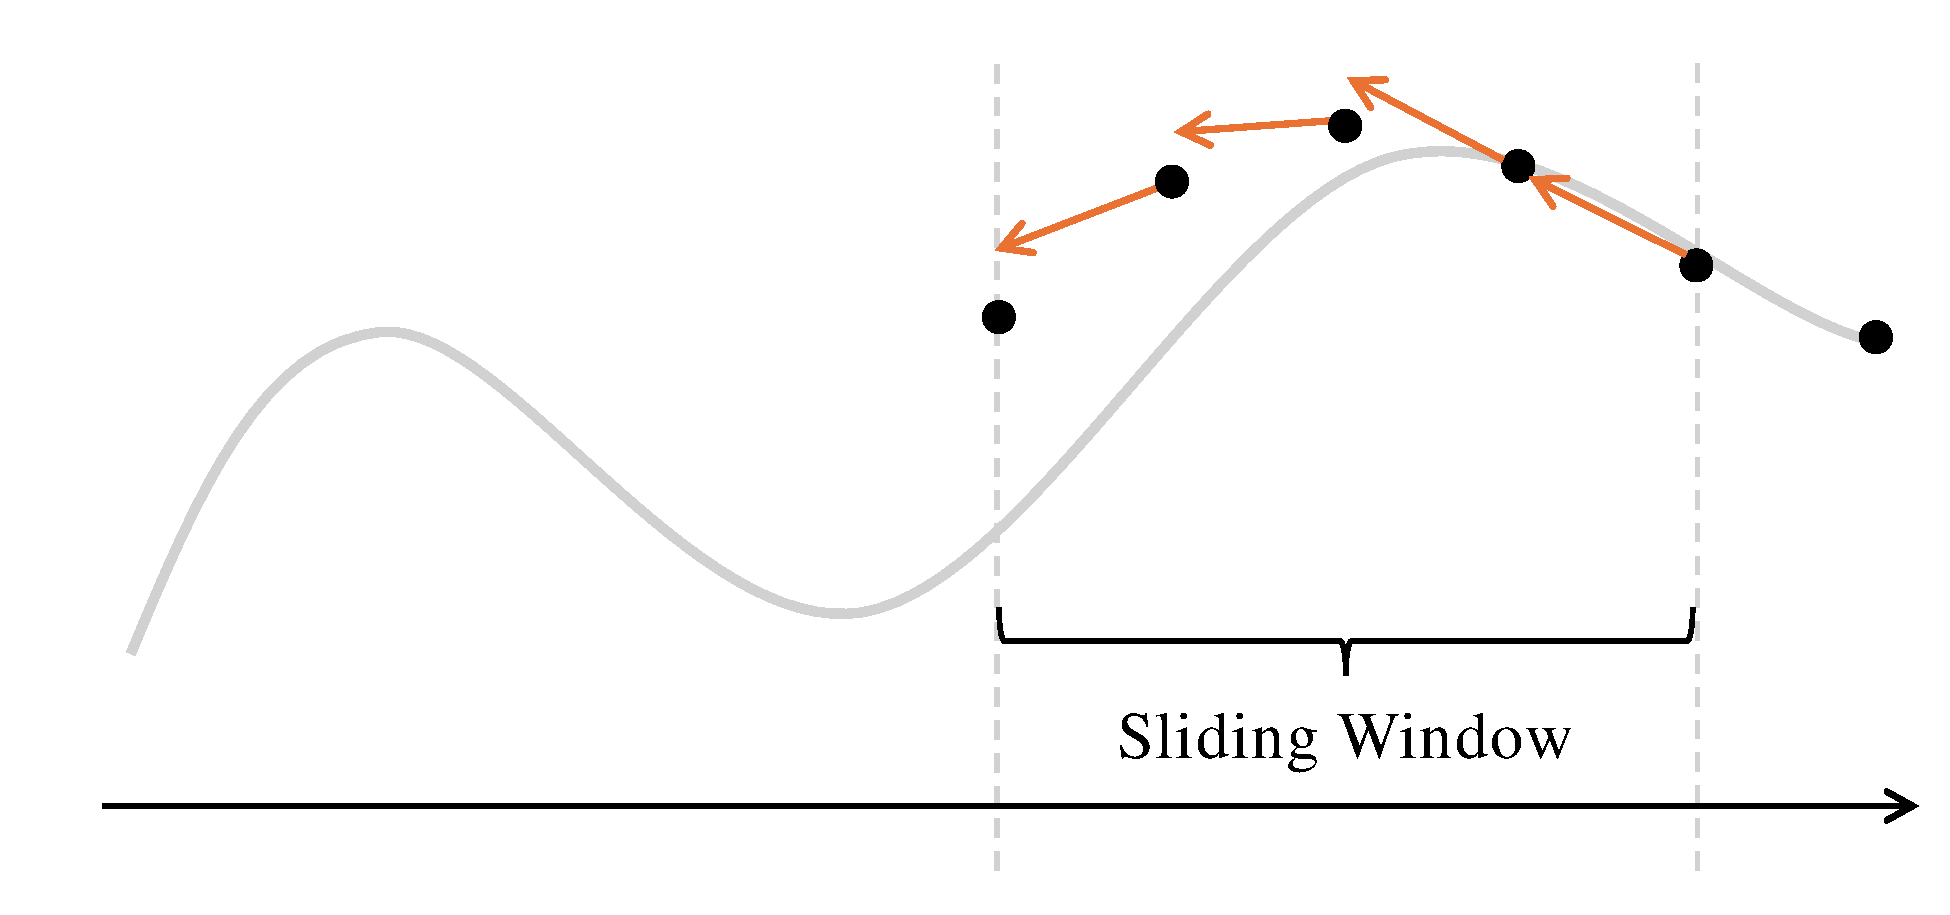
\includegraphics[width=\linewidth]{Images/PartC/paradigm-1.pdf}
        \caption{Compute the drift of $\rvx^{(k)}_{\ell:\ell+p}$ on a batch window of size $p=4$, in parallel}
        \label{fig:picard_1}
    \end{minipage}%
    \hspace{0.03\textwidth} % To maintain the space between the images
    \begin{minipage}[t]{0.30\textwidth}
        \centering
        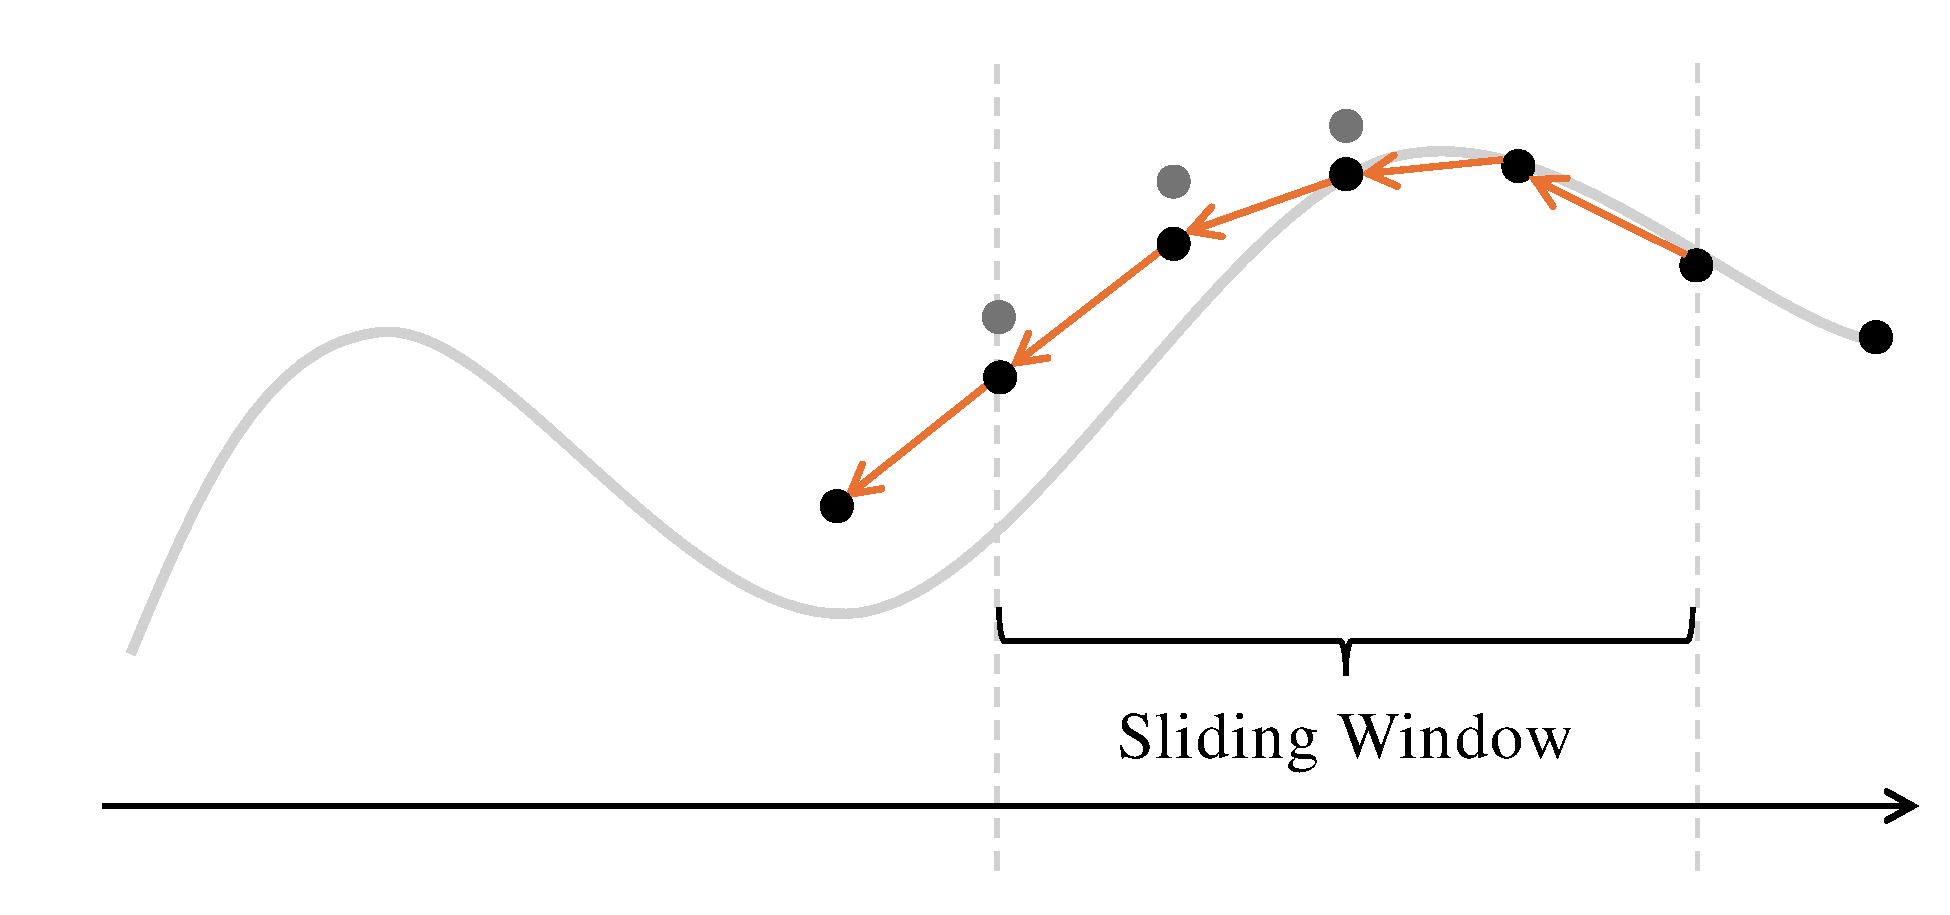
\includegraphics[width=\linewidth]{Images/PartC/paradigm-2.pdf}
        \caption{Update the values to $\rvx^{(k+1)}_{\ell:\ell+p}$ using the cumulative drift of points in the window}
        \label{fig:picard_2}
    \end{minipage}%
    \hspace{0.03\textwidth} % To maintain the space between the images
    \begin{minipage}[t]{0.30\textwidth}
        \centering
        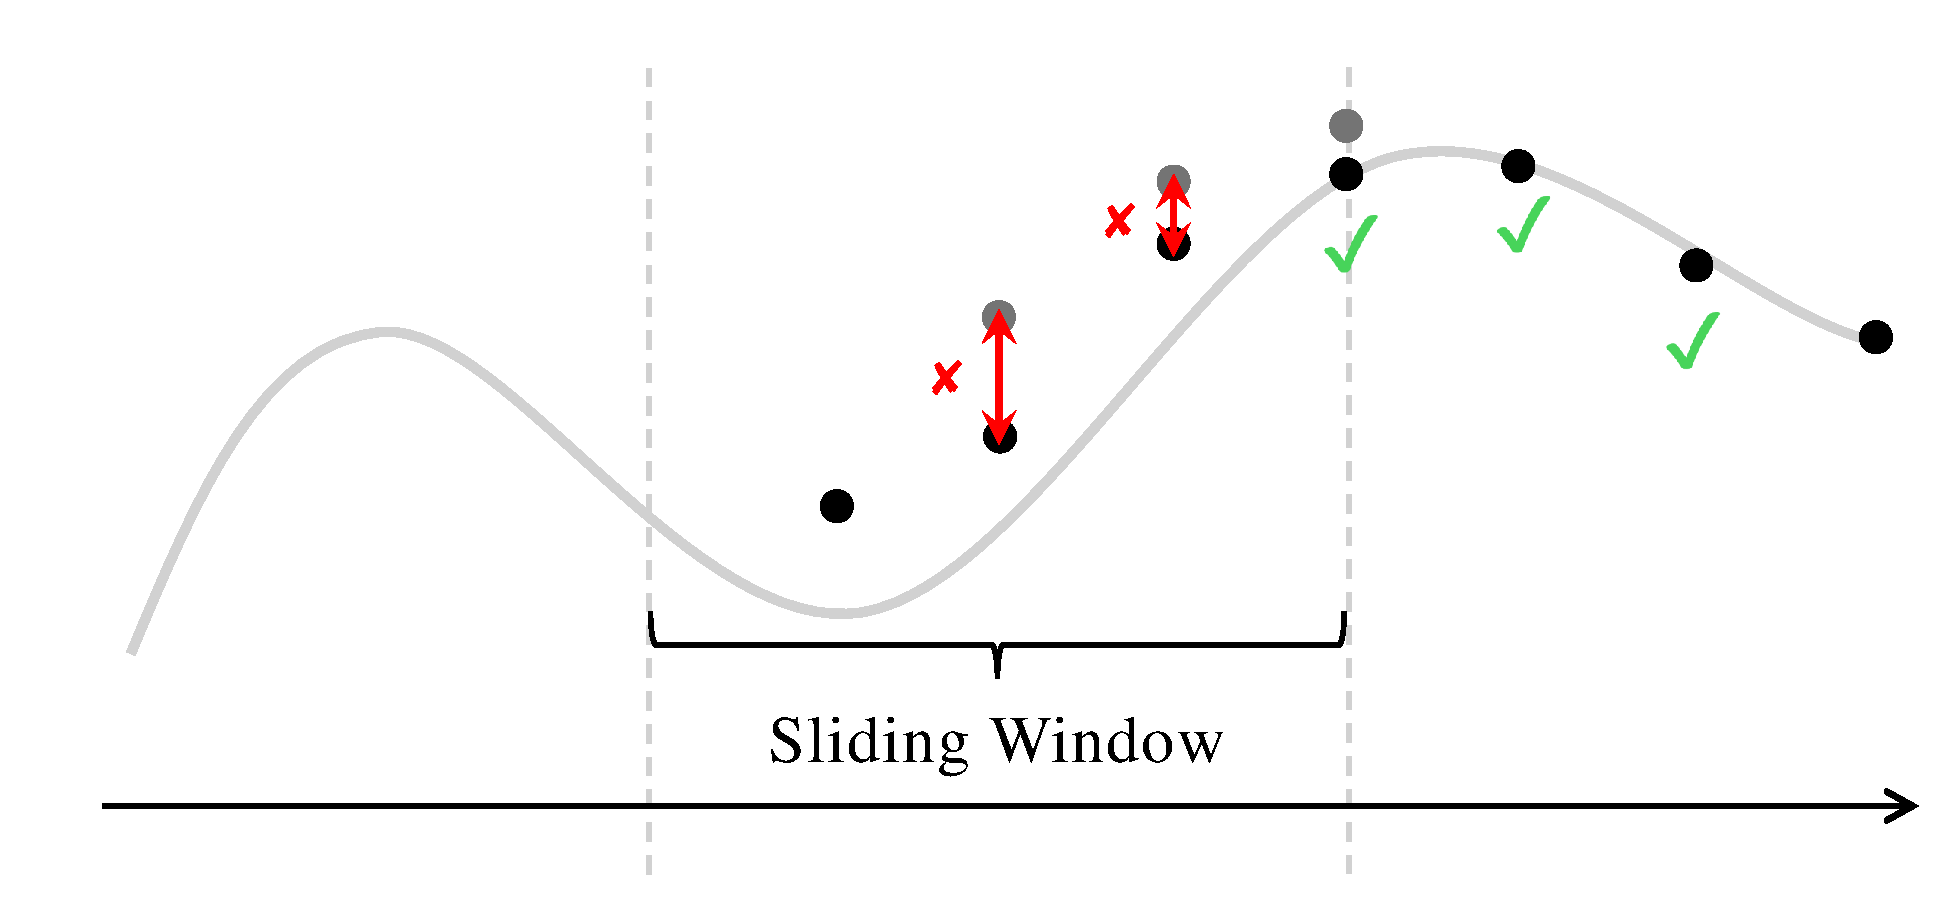
\includegraphics[width=\linewidth]{Images/PartC/paradigm-3.pdf}
        \caption{Determine how far to slide the window forward, based on the error $\lVert \rvx^{(k+1)}_i - \rvx^{(k)}_i \rVert^2$.}
        \label{fig:picard_3}
    \end{minipage}
    % \caption{During iteration $k$, ParaDiGMS processes a batch window of size $p$ spanning timesteps $[t,t+p)$ \textit{in parallel}. The new values at a point $\rvx^{(k+1)}_{t+j}$ are updated based on the value  $\rvx^{(k)}_j$ at the left end of the window, plus the cumulative drift  $1/T \sum_{i=t}^{t+j-1} \mathbf{F}_{\bm{\phi}^\times}(\rvx^{(k)}_{i}, i/T)$  of points within the window. We then slide the window forward until the error exceeds our tolerance, and repeat for the next iteration.}
    \figcredit{Adapted from \citet{shih2023parallel}.}
    \label{fig:picard}
\end{figure}


The discrete Picard update \Cref{eq:discrete_picard_decreasing} expresses each $\rvx^{(k+1)}_j$ as the left–anchored value $\rvx^{(k)}_0$ minus a cumulative sum of drifts. To limit memory and exploit parallel hardware, it is convenient
to apply the same idea  locally on short, sliding blocks of indices.

Fix a window length $p$ and a left index $\ell$; the window then covers
$j=\ell,\ldots,\ell+p$ with $t_\ell>t_{\ell+1}>\cdots>t_{\ell+p}$. During
iteration $k$:

\subparagraph{Step 1. Parallel Drift Evaluation on the Window.}
Compute, in parallel and using only the previous iterate,
\[
\rvv_{\bphi^\times} \big(\rvx^{(k)}_{\ell+i}, t_{\ell+i}\big),
\quad i=0,1,\ldots,p-1.
\]
These are the $p$ local increments needed to advance from the left edge
$t_\ell$ across the window.

\subparagraph{Step 2. Left–Anchored Cumulative Updates.}
Form the windowed updates by anchoring at $j=\ell$ and accumulating the drift across subintervals:
\begin{equation}\label{eq:window_update}
\rvx^{(k+1)}_{\ell+j+1}
 = 
\rvx^{(k)}_{\ell}
 - \Delta t \sum_{i=0}^{j}
\rvv_{\bphi^\times} \big(\rvx^{(k)}_{\ell+i}, t_{\ell+i}\big),
\quad j=0,1,\ldots,p-1.
\end{equation}
This is precisely \Cref{eq:discrete_picard_decreasing} restricted to the
window, with the minus sign reflecting the decreasing time direction. The inner
sum is a prefix-sum (scan) over the windowed drifts, so all partial sums
can be produced efficiently on parallel hardware.

\subparagraph{Step 3. Progress Control and Window Advance.}
Having formed the left–anchored cumulative updates on the current window (Step~2),
we now decide how far to slide that window. We measure local convergence
by the pointwise Picard change
\[
\mathtt{error}_j
:=
\big\|\rvx^{(k+1)}_{\ell+j}-\rvx^{(k)}_{\ell+j}\big\|^2,
\quad j=1,\ldots,p-1,
\]
and compare it against prescribed tolerances $\mathtt{tol}_{\ell+j}$. That is, $\mathtt{error}_j$ measures how much the iterate at node $\ell+j$ changed during the last Picard
update. If this number is small, it indicates local agreement between the two
successive approximations and hence local convergence of the fixed-point
iteration at that node. If it is large, that node has not settled yet and needs
more Picard smoothing.


The \emph{stride} is chosen as the first index in the window that fails this
test (or the full window length $p$ if none fail):
\[
\mathtt{stride}
:=
\min\Big(\,\{\,j\ge 1:\ \mathtt{error}_j>\mathtt{tol}_{\ell+j}\,\}\ \cup\ \{p\}\Big).
\]
We then slide the window by setting $\ell \leftarrow \ell+\mathtt{stride}$.  In words: we accept all nodes from the left edge up to (but not including) the
first one that has not converged; if all nodes have converged, we accept the
entire window. We then slide the window by that many accepted nodes,
$\ell \leftarrow \ell+\mathtt{stride}$, and continue. This advances by at
most the window length $p$, never skipping any node that has not met its
tolerance. If sliding would overrun the grid end $M$, we truncate the window to
$p \leftarrow \min\{p,\,M-\ell\}$ and proceed.



When the window moves forward it uncovers new time nodes that
have no values yet. To start Picard iteration there, we simply copy the value
from the left boundary of the window and use it as an initial guess. This
``constant extrapolation'' is cheap and stable, and will be corrected by later
updates. If desired, one can replace it by more accurate guesses, such as linear
or polynomial extrapolations from past points.

This completes the procedure of ParaDiGMS. We summarize the algorithm in \Cref{alg:paradigms}.


\begin{algorithm}[t]
  \caption{ParaDiGMS with Sliding Windows}
  \label{alg:paradigms}
  \begin{algorithmic}[1]
    \Require Drift $\rvv_{\bphi^\times}(\rvx,t)$; $\{t_j\}_{j=0}^{M}$; window length $p$; $\{\mathtt{tol}_j\}_{j=1}^{M}$
    \Ensure Approximate trajectory $\{\rvx^{(k)}_j\}_{j=0}^{M}$ with $\rvx^{(k)}_M$ at $t=0$
    \State $k \gets 0$, $\ell \gets 0$ 
    \State Sample $\rvx^{(0)}_0 \sim p_{\mathrm{prior}}$; set $\rvx^{(0)}_j \gets \rvx^{(0)}_0$ for $j=1,\ldots,\min(p,M)$  \Statex \Comment{constant extrapolation}
    \While{$\ell < M$}
      \State $J \gets \min(p,  M-\ell)$   \Comment{current window length}
      \State \textbfs{Step 1: Parallel} 
      \State For $i=0,\ldots,J-1$: $g_i \gets \rvv_{\bphi^\times} \big(\rvx^{(k)}_{\ell+i},\, t_{\ell+i}\big)$ 
      \Statex \Comment{drifts from previous iterate (Picard freezing)}
      \State Compute prefix sums $S_j \gets \sum_{i=0}^{j} g_i$ for $j=0,\ldots,J-1$ 
      \Statex \Comment{scan over windowed drifts}
      \State \textbfs{Step 2: Cumulative Updates} 
      \State For $j=0,\ldots,J-1$: $\displaystyle \rvx^{(k+1)}_{\ell+j+1} \gets \rvx^{(k)}_{\ell} - \Delta t\, S_j$ 
      \Statex \Comment{left-anchored update; cf.\ \Cref{eq:window_update}}
      \State \textbfs{Step 3: Progress Control and Window Advance} 
      \State For $j=1,\ldots,J-1$: $\mathtt{error}_j \gets \big\|\rvx^{(k+1)}_{\ell+j}-\rvx^{(k)}_{\ell+j}\big\|^2$ \Statex \Comment{pointwise Picard change}
      \State $\displaystyle \mathtt{stride} \gets \min \Big(\,\{\,j\in\{1,\ldots,J-1\}:~\mathtt{error}_j>\mathtt{tol}_{\ell+j}\,\}\ \cup\ \{J\}\Big)$
      \State \textbfs{Initialize New Nodes} 
      \State For $r=1,\ldots,\mathtt{stride}$: $\rvx^{(k+1)}_{\ell+J+r} \gets \rvx^{(k+1)}_{\ell+J}$ 
      \Statex \Comment{constant extrapolation into newly exposed indices}
      \State $\ell \gets \ell + \mathtt{stride}$;\quad $k \gets k+1$
    \EndWhile
    \State \Return $\{\rvx^{(k)}_j\}_{j=0}^{M}$
  \end{algorithmic}
\end{algorithm}




\subsection{Relation to Time-Stepping Solvers}

\paragraph{Selection of Sliding Window Size.}

To place the sliding window scheme in context, note first what happens at the
smallest window size. When $p=1$, the window contains a single step, so
\Cref{eq:window_update} collapses to a first–order time-stepping update of the
PF–ODE. The method reduces to, for instance, DDIM, if we use the same way of writing the ODE (e.g. data vs. noise prediction) and choose the same schedule of discrete timesteps as in DDIM.

Increasing $p$ expands parallelism (more nodes advanced per window) without
changing the overall step count $M$. Consequently, sample quality continues to
be determined by the base discretization (choice of grid/parameterization
and per–step formula) together with Picard convergence on each window,
which we monitor via the local tolerances. 

\paragraph{Compatibility with Higher–Order Solvers (e.g., DPM).}
The sliding–window Picard structure controls \emph{how} increments are computed
(in parallel and accumulated by a scan), not \emph{which} local formula defines
those increments. Consequently, one may replace the left–endpoint rule by any
consistent higher–order quadrature without changing the parallel
layout. For example, a trapezoidal variant of \Cref{eq:window_update} reads
\begin{align*}
    \begin{aligned}
        \rvx^{(k+1)}_{\ell+j+1}
=
\rvx^{(k)}_{\ell}
-\Delta t \Big[
\tfrac{1}{2}\rvv_{\bphi^\times} \big(\rvx^{(k)}_{\ell},t_{\ell}\big)
+\sum_{i=1}^{j-1}\rvv_{\bphi^\times} \big(\rvx^{(k)}_{\ell+i},t_{\ell+i}\big)
+\tfrac{1}{2}\rvv_{\bphi^\times} \big(\rvx^{(k)}_{\ell+j},t_{\ell+j}\big)
\Big],
    \end{aligned}
\end{align*}
where all drifts are still taken from the previous Picard iterate, so
the per–node evaluations remain independent and the inner sum remains a prefix–sum.

Likewise, multistep or exponential–integrator updates used by DPM solvers family
(e.g., DPM–Solver\texttt{++} $2$M in log–SNR time) can be inserted by
replacing each windowed increment with the corresponding higher–order linear
combination of past model evaluations ($\rvx$- or $\beps$-predictions with precomputed
coefficients). The scan then accumulates those weighted increments across the
window exactly as before. In short: the parallel scheme is independent of the solver (discretization) choice to approximate the integral. Accuracy comes from the base solver; the windowed prefix–sum just makes it fast.

\newpage
\section{Closing Remarks}\label{sec:ch9_cr}

This chapter has confronted one of the most significant practical limitations of diffusion models: their slow, iterative sampling process. We have explored a powerful class of training-free solutions that accelerate generation by leveraging the rich field of numerical methods for differential equations. The core strategy has been to more efficiently solve the PF-ODE, which defines the deterministic generative trajectory from noise to data:
\begin{enumerate}
    \item We began with the foundational DDIM, which can be understood as a first-order exponential Euler method.
    \item We then moved to higher-order multi-step methods like DEIS, which improve accuracy by using a history of past evaluations.
    \item Finally, we examined the highly efficient DPM-Solver family, which achieves remarkable performance by introducing a crucial log-SNR time reparameterization.
\end{enumerate}

Through these sophisticated solvers, the number of function evaluations (NFEs) required for high-quality generation has been dramatically reduced from hundreds or thousands to as few as 10-20, making diffusion models significantly more practical.

However, these training-free methods are still fundamentally iterative. They approximate a continuous path step-by-step. This raises a natural and ambitious question: \emph{can we achieve high-quality generation in just one or a very few discrete steps?}

The final part D of this monograph will explore this question through training-based acceleration. We will investigate two main strategies:
\begin{enumerate}
    \item First, in \Cref{ch:distillation}, we will examine distillation-based methods, where a fast \textit{student} generator is trained to replicate the output of a slow, pre-trained \textit{teacher} diffusion model in far fewer steps.
    \item Then, in \Cref{ch:fast-scratch}, we will push this idea further by exploring methods that learn fast, few-step generators from scratch, such as Consistency Training, which define a standalone training principle without relying on any pre-trained model.
\end{enumerate}

This shift from improving the solver to learning the solution map itself represents the frontier of efficient generative modeling, aiming to combine the quality of diffusion models with the speed of one-step generators. 


% \begin{itemize}
%     \item When $p=1$, ParaDiGMS reduces to the Euler method, equivalent to DDIM.
%     \item ParaDiGMS is compatible with any time-stepping ODE solver, including DDIM, DEIS, and the DPM-solvers family, among others.
%     \item ParaDiGMS does not degrade sample quality as it does not aim to reduce the number of sampling timesteps. 
% \end{itemize}


\clearpage
\newpage
